% Class options:
%  Font size: 10pt, 11pt, 12pt (default is 11pt)
%  Paper sides: oneside, twoside (default is oneside)
% The default options conform to UoY regulations; keep these unless there is a good reason to do otherwise.
\documentclass[11pt,oneside]{yorkcsthesis}

% Formatting specifications for University of York theses
% as specified in Regulation 2.8 'Theses submitted for higher degrees' (based on ISO 4821:1990)
% Contains elements of M. Imran's template for University of Durham, Department of Mathematics

% Load useful packages here; you _must_ include 'fancyhdr'
\usepackage{fancyhdr}

% hyperref must be called BEFORE apacite
\usepackage{hyperref}
\usepackage{acronym}
\usepackage{afterpage}
\usepackage{algorithm}
\usepackage{algorithmic}
\usepackage{amsfonts}
\usepackage{amsmath}
\usepackage{amssymb}

\usepackage[notocbib,nosectionbib]{apacite}
% let the doi package handle stuff
\renewcommand{\doiprefix}{}
\usepackage[UKenglish]{babel}

\usepackage{booktabs}
\usepackage[font=small,
			labelfont=bf,labelsep=period]{caption}
\usepackage{doi}
\usepackage{epic}
\usepackage{epsfig}
\usepackage{framed, color}
\definecolor{shadecolor}{rgb}{0.8,0.8,0.8}
\usepackage{graphicx}
\usepackage{ifthen}
\usepackage{latexsym}
\usepackage{multicol} 
\usepackage{multirow}
\usepackage[super]{nth}
\usepackage{paralist}
\usepackage{pdfpages}
\usepackage{rotating}
\usepackage{siunitx}
\usepackage{subfigure}
\usepackage{theorem}
\usepackage[flushleft]{threeparttable}
\usepackage{units}
\usepackage{wrapfig}

% Select fonts here; leave all commented to use LaTeX defaults (Computer Modern family)
% I found Computer Modern family really difficult to read on screen
% Note that some fonts tend to give bigger pagecounts: Times < Palatino < ComputerModern < NewCenturySchoolbook
%\usepackage{fontenc}
%\usepackage{times}	% Times, Helvetica, Courier
%\usepackage{newcent}	% New Century Schoolbook, Avant Garde, Courier
%\usepackage{palatino}	% Palatino, Helevetica, Courier

% Uncomment this line to use the selected sans-serif font for the main body text. You probably don't want to do this.
%\renewcommand{\familydefault}{\sfdefault}

% fancy header
\pagestyle{fancy}
\renewcommand{\chaptermark}[1]{\markboth{\chaptername\ \thechapter:\ #1}{}}
\renewcommand{\sectionmark}[1]{\markright{\thesection\ #1}}
\lhead[\fancyplain{}{\leftmark}]	{\fancyplain{}{}}
\chead[\fancyplain{}{}]			{\fancyplain{}{}}
\rhead[\fancyplain{}{}]			{\fancyplain{}{\rightmark}}
\lfoot[\fancyplain{}{}]			{\fancyplain{}{}}
\cfoot[\fancyplain{}{\thepage}]		{\fancyplain{}{\thepage}}
\rfoot[\fancyplain{}{}]			{\fancyplain{}{}}

% theorem style
{\theorembodyfont{\rmfamily}\newtheorem{Pro}{{\textbf Proposition}}[section]}
{\theorembodyfont{\rmfamily}\newtheorem{The}{{\textbf Theorem}}[section]}
{\theorembodyfont{\rmfamily}\newtheorem{Def}[The]{{\textbf Definition}}}
{\theorembodyfont{\rmfamily}\newtheorem{Cor}[The]{{\textbf Corollary}}}
{\theorembodyfont{\rmfamily}\newtheorem{Lem}[The]{{\textbf Lemma}}}
{\theorembodyfont{\rmfamily}\newtheorem{Exp}{{\textbf Example}}[section]}
\def\remark{\textbf{Remark}:}
\def\remarks{\textbf{Remarks}:}
\def\bproof{\textbf{Proof}: }
\def\eproof{\hfill$\Box$}
% Line spacing tweaks
% UoY thesis demands 1.5x but sometimes we need to drop to 1.0x in tables, algorithms, and other awkward elements.
% Call \linespacesmall before the table, then \linespacenormal after the table.
\def\linespacesmall{
\renewcommand{\baselinestretch}{1.0}
}
\def\linespacenormal{
\renewcommand{\baselinestretch}{1.5}
}

% declaration text
% full references in text are all hand-edited. Package bibentry and hyperref have an unsolved conflict. To enable hyperref, I chose not to use bibentry.
\def\contentdeclaration{

I, Hao-Ting Wang, declare that this thesis is a presentation of original work and I am the sole author. I undertook the research at University of York during \yearstartedtext{} -- \yearendedtext{}, under the joint supervision of Professor Jonathan Smallwood and Professor Elizabeth Jefferies. This work has not previously been presented for an award at this, or any other, University. All sources are acknowledged as References.

Some parts of this thesis have been published in peer-reviewed journals or is currently under preparation for publication. Author contributions are noted at the start of each chapter.  

\begin{itemize}
    \item \cref{ch:methods}: Wang, H.-T., Smallwood, J., Satterthwaite, T. D., Bassett, D. S., \& Bzdok, D. (2018). Finding the needle in high dimensions: A tutorial on CCA in biomedicine. Manuscript preparing for publication.	
	\item \cref{ch:study1}: Wang, H.-T., Poerio, G. L., Murphy, C. E., Bzdok, D., Jefferies, E., \& Smallwood, J.(2018). Dimensions of Experience: Exploring the Heterogeneity of the Wandering Mind. \textit{Psychological Science}, \textit{29} (1), 56--71. doi: \url{10.1177/0956797617728727}
	\item \cref{ch:study2}: Wang, H.-T., Bzdok, D., Margulies, D. S., Craddock, C., Milham, M., Jefferies, E., \& Smallwood, J.(2018). Patterns of thought: Population variation in the associations between large-scale network organisation and self-reported experiences at rest. \textit{NeuroImage}, \textit{176} (1), 518--527. doi: \url{10.1016/j.neuroimage.2018.04.064}
\end{itemize}

}

% acknowledgements text
\def\contentacknowledgement{

The most exciting chapter of my academic journey would not be possible without my supervisors Prof. Jonathan Smallwood and Prof. Elizabeth Jefferies. Jonny and Beth are the kindest people I have ever known. Especially, I cannot be more thankful for Jonny's trust in me when I was doubtful of my own ability. That offer really changed my life. Their help and support in both science and life have made this PhD a truly rewarding experience. From them, I learned to be a better scientist and also a good person. 

I express my gratitude to Prof. Dr. Dr. Danilo Bzdok for the guidance and discussions on the canonical correlation analysis project. Our discussions at various Brainhacks helped tremendously in the research methods of this PhD. 

I thank my thesis advisory panel, Dr. Tom Hartley, Dr. Aidan Horner, and Dr. Cade McCall for providing a friendly environment to discuss science and my skill development. 

All the research projects presented here will not be possible without the current and past members of semantics and thought lab. Their contributions lie not just in the research, and also moral supports on my personal life. Good colleagues like them are difficult to come by. 

Finally, thanks to all my family and friends for all their assistance. The special mentions go to Thomas Hardman and Rebecca Jones for making my life more fun in general. 

}

% acronyms and abbreviations text
\def\contentabbreviations{\indent 
 \begin{acronym}[ANOVA] % put the longest/widest acronym between the square brackets; it defines the left hand column width
 \acro{ANOVA}{ANalysis Of VAriance}
 \acro{CCA}{Canonical Correlation Analysis}
 \acro{DMN}{Default Mode Network}
 \acro{ERP}{Event-Related Potential}
 \acro{fMRI}{Functional Magnetic Resonance Imaging} 
 \acro{PCA}{Principle Component Analysis}
 \acro{MDES}{Mulit-Dimension Experience Sampling}
 \acro{SCCA}{Sparse Canonical Correlation Analysis}
\end{acronym}
}

% abstract text
\def\contentabstract{
Functional outcomes of ongoing thought show both costs and benefits. Yet, the reason for its heterogeneity remains unclear. The executive failure and representational accounts stemmed from different psychological research approaches to understand ongoing thought. The executive failure account examines why changes in ongoing thought happen, while the representational account seeks to explain how human generates ongoing thought. The attentional system and the default mode network are the common neural processes of both theoretical accounts, but interacting in a contradicting manner. The two accounts can be seen as competing theories of ongoing thought. However, in the family resemblance view \cite{Seli2018}, the two theoretical accounts potentially serve as two component processes of one phenomenon. One possible solution to this conflict could be that under different global neural configurations, the two networks support different cognitive functions. The thesis sets out to present evidence supporting of the family resemblance view and to begin research on the ontology of the component processes in ongoing thought. Neural cognitive hierarchy is the potential explanation of the heterogeneity. The current thesis adopts sparse canonical correlation analysis to incorporate the neural and behavioural aspects of ongoing thought. The data suggests ongoing thought is a collective phenomenon with many types of experience driven by the connectivity patterns in the default mode network. Each type of experience associated with their unique functional outcomes and neural hierarchies at the whole-brain level. Cognitive flexibility and the balance of segregation and integration between the transmodal systems and the rest of the cortex determines the immersive details. The current findings suggested the importance of whole-brain neural hierarchies to ongoing thought. The confirmation of these trait level findings at a state level are necessary to gain more insights into the architecture of the component processes.
}


% Shortcuts and assorted macros
\def\mparetasquared{\eta_{p}^{2}}
\def\paretasquared{$\eta_{p}^{2}$}

\makeatletter
\newcommand*{\rom}[1]{\expandafter\@slowromancap\romannumeral #1@}
\makeatother


% Math operators and function names
\DeclareMathOperator{\avg}{avg}
\renewcommand{\vec}[1]{\mbox{$ \overrightarrow{ #1 } $}}

% add details about your thesis here
\author{Hao-Ting Wang}
\title{Towards an Ontology of Ongoing Thought}
\degree{PhD}
\department{Psychology}
\date{September 2018}
\yearstarted{2015}
\yearended{2018}
\abstract{\contentabstract}
\acknowledgements{\contentacknowledgement}
\declaration{\contentdeclaration}
\abbreviations{\contentabbreviations}

% when working on a chapter, removing other chapters from this list suppresses compilation and hence reduces thesis compile time
%\includeonly{study1/main}

\begin{document}

%document
\pagenumbering{roman}
\maketitle
\setcounter{page}{2} % count the title page as pp1

\makeabstract

\tableofcontents
\listoffigures
\listoftables

\makeacknowledgements
\makedeclaration


\cleardoublepage
\pagenumbering{arabic}
\setcounter{page}{1}

% include your chapters here
\chapter{Introduction}
\label{ch:intro}
\chaptermark{Introduction}

%\setcounter{equation}{0}
% ==========================================================================================================

Recent advance on studies of on-going thought is driven by the popularisation of functional magnetic resonance imaging (fMRI), combined with established psychological researches. The increasing researches showed heterogeneous views on how and why mind wandering occurs, however the underlying mechanism is rather unexplored. The current thesis explores the patterns of on-going thought extending from well-studies category---mind wandering---to task-related thought. The aim is to gain an understanding of the component processes of on-going thought at task and rest. A flexible family resemblance view \cite{Seli2018} of on-going thought will joint the identified patterns of the shared similarities, as well as unique features that drives the heterogeneity.

In this chapter, I walk through the conflicting behavioural literature of mind wandering and discuss the theoretical accounts of on-going thought. Next I introduce the emerging neural evidence on hierarchical organisation that suggests how overlapping component processes might facilitate on-going thought. In closing, I introduce the overall methods used in the current research and how a multivariate approach helps to examine the family resemblance view.

\section{Heterogeneity of on-going thought}
\label{ch:intro:heterogeneity}
\sectionmark{Heterogeneity}

% lay out the component processing account and family resemblance view

With the advance of fMRI and other neuroimaging technique, the study of on-going thought has gained wider interest in psychology and neuroscience in the past decade. Mind wandering is particularly well-studied among all phenomena related to on-going thoughts. Researchers aim at understanding how the mind shifts between external environment and internal thoughts unrelated to the here-and-now. 
The executive failure account is concerned with why some mind wandering episodes occur to the detriment of the integrity on-going task. In contrast to the executive failure view, the representational account seeks an understanding of how the mental content is generated. The two approaches have led to a conflicts in the mind wandering literature. In a family resemblance view, members of the on-going thought family can have shared similarities along with unique features resulting the heterogeneity. The following section will introduce the evidence for construct overlap and shared processes of on-going thought at task and rest.

\subsection{Heterogeneity in definitions}
Among types of on-going thought, mind wandering attracted the most interest as it concerns the ability to focus on task at hand. Mind wandering has been studied in a variety of related psychological domains, such as cognition, emotion, and neuroscience. Various lines of research have addressed the basic phenomenal characteristics of mind wandering---
\begin{quote}
    \textit{a shift in the contents of thought away from an ongoing task and/or from events in the external environment to self-generated thoughts and feelings.}\\    
    \cite{SmallwoodSchooler2006,SmallwoodSchooler2015}.
\end{quote}
We are all familiar with moments when the train of thought shift away from the tasks at hand, and sometimes getting annoyed by the mind wandering episode. The intuition has lead to researches describing mind wandering as an `attentional lapse' \cite{McVayJOEP2009, McVay2012}, implying the occurrence of mind wandering is an unintended failure. When the study explicitly instruct the participant to perform a task, the time not focusing on the task are considered as `mind wandering'. Such research design dismissed the possibility of voluntary engagement of the mind wandering state. 

Recent investigations have found that mind wandering can occur with or without intention \cite<see review from>{SeliTiCS2016}. The participant can intentionally mind wander if they lack a motivation to engage in the experiment. When a simple yes/no question is asked about the mind wandering state, the response cannot access the nature of the occurrence. When participants are asked about the nature of mind wandering period in laboratory scenario, less than half of the mind wandering period is intentional \cite{SeliJoEP2015}due to the lack of motivation to complete the task \cite{SeliJoEP2015}, or the task is not mentally demanding to have all the attention resource allocated to the task \cite{SeliPsychScience2016}. The occurrence of intended and unintended mind wandering can also be down to individual differences. Intentional and unintentional mind wandering have been found to be deferentially associated with attention-deficit/hyperactivity disorder \cite<ADHD;>{SeliADHD2015} and obsessive-compulsive disorder \cite<OCD;>{SeliOCD2017}. The work on the intention of mind wandering demonstrates that there is indeed overlap in the various definitions, and that other components that contribute to the heterogeneity. 

\subsection{Heterogeneity in functional outcomes}

The family resemblance view suggests that complex thought can emerge from the combination of multiple overlapping processes. A myriad of mind wandering researches concern the functional outcomes. The current thesis proposes that the heterogeneous functional outcomes are evidence in support of a variety of component processes underlying the on-going thought. 

Mind wandering has been associated with poor executive control during working memory task \cite{McVayJOEP2009}. Individuals who mind-wandered more during fluid intelligent testing perform less well \cite{MrazekJoEP2012}. Mind wandering leads to bad reading comprehension due to failure in the construction of the mental models of ongoing events \cite{Smallwood2008}. Comprehension ability is related to working memory capacity and mediated by the ability to suppress mind wandering \cite{McVayReading2012, Unsworth2013}. Mind wandering has been linked to unhappiness \cite{Killingsworth2010} and a indicator of depression \cite{Smallwood2007}. The evidence above supported the highly disruptive nature of mind wandering and its potential costs to cognitive performance.

In addition to exploring the costs of mind wandering, researchers have discovered its potential benefits. Mind wandering may facilitate creative solution to an old problem \cite{Baird2012, Smeekens2016} and recovery from negative emotional states \cite{RubyPlos2013, PoerioFrontiers2016}. Mind wandering relays on mental time travel---the metal capacity of remembering the past and imagining the future \cite{Stawarczyk2015}.  Mind wandering can refine personal goals \cite{Medea2016} and is associated with the neural mechanism supporting mental time travel \cite{DArgembeau2006,DArgembeau2015}. 

Different functional associations arise from the same type of experience---mind wandering. To reconcile this contradictory evidence, researchers have suggested that mind wandering may encompasses multiple states with differential contents and underlying cognitive architectures \cite{SmallwoodFrontiers2013}. Complex thought can emerge from the combination of multiple overlapping processes. 

\subsection{Heterogeneity in experiential profiles}

Self-report is commonly used to understand the content of mind wandering thoughts and on-going experience. The content of mind wandering has a wide variety of topics and modality. The questions in the report address a number of dimensions of the on-going experience, ranging from the state of attention, temporal content, social content and modality. Principle component analysis (PCA) formalised the statistically shared association between the different aspects of the reports. 

Studies using PCA on such experience reports have revealed more detailed experiential profiles. Temporal information is one common theme \cite{RubyFP2013,RubyPlos2013}. The content of mind wandering is mainly future-focused \cite{Baird2011}, therefore mind wandering often involves planning for the future goals of the individual. On the contrary, when the mind wanders in an unhappy mood, the content is drawn to events from its past \cite{Smallwood2011}. The form of spontaneous thoughts is likely to be imagery or verbal \cite{Gorgolewski2014,Smallwood2016}. 

The positive/negative-valence of emotion of thought has tendency to accompany with different temporal directions. These unique associations discovered through PCA suggested the component processes at a experiential level. Investigation in experiential profiles is the first step to explore the commonality of various type of on-going thought. 

% ==========================================================================================================

\section{Theoretical accounts of mind wandering}
\sectionmark{Theoretical accounts}
\label{ch:intro:accounts}

The heterogeneity of mind wandering has been formalised into two theoretical accounts. The executive failure account aim to understand the conditions that trigger or associate with on-going thought. Researches on the mechanism behind the occurrence of on-going thought is the representational account. In other words, the executive failure account examines why changes in on-going thought happens, while the representational account interests in how human generates on-going thought while mind wandering. The two accounts can been seen as competing theories of mind wandering. However, in a family resemblance view, the two theoretical account supports the idea that the potential of a singular phenomenon is composed of multiple underlying component processes. 
\subsection{Executive failure account}
The executive failure account is concerned with a single aspect of mind wandering, namely understanding why some mind wandering episodes occur to the detriment of the integrity on-going task. Mind wandering occurs during attention-demanding tasks when control processes are insufficient to deal with the interference created by off-task thoughts \cite{Kane2012,McVay2010}. Mind wandering results from a failure of executive control over internally generated thoughts, rather than as consuming executive resources. The researches focus on the negative effect of mind wandering on the development of negative mood and task performance. Mind wandering thoughts are mostly unhappy in ecologically valid scenario \cite{Killingsworth2010}. Depressive thinking correlates with the frequency of mind wandering \cite{Smallwood2007}. 

In the executive failure view, mind wandering reflects momentary lapse in attention. The definition of attention lapse is a relatively slow response time to the task at hand, which is consistent with the mind wandering indicator used in working memory capacity research \cite{McVay2012}. Mind wandering has been considered the reason of poor executive control during working memory task \cite{McVayJOEP2009}. Executive error and slow reaction time correlates with individual differences in working memory capacity and mind wandering \cite{McVay2012}. The capacity to avoid mind wandering during demanding tasks is a potentially important source of success on measures of fluid intelligence \cite{MrazekJoEP2012}. 

% neural basis
Task-based fMRI study on attention lapse has contributed the functional neural processes to support the executive failure account. \citeA{Weissman2006} have uncover the neural mechanism behind the attention lapse during a global/local selective-attention task. Brief attention lapse is related t early activity in frontal control region including anterior cingulate cortex (ACC), right middle frontal gyrus (MFG), and right inferior frontal gyrus (IFG). Attention laspse also suggested the failure of maintaining perceptual representation. Reduced activity is found in primary visual area. Activation of default mode network \cite<DMN; >{Raichle2001} has been observed during a brief attention lapse. DMN is a set of brain regions composed of medial prefrontal cortex(MPFC), and posterior cingulate coretex (PCC) as the core and subsystems on medial and lateral regions of the temporal lobe. DMN is commonly referred as a task-negative network\cite{Fox2005}, associating with task-unrelated thought and mind wandering \cite{MasonScience2007,Christoff2009}. The lapses leads to demands on the frontal-parietal control relate regions for redirecting attention. Ventral frontal-parietal regions, including right temporal-parietal junction (TPJ) and right IFG, for recovery from lapses. 

\subsection{Representational account}

The representational account concerns the generation of content during mind wandering, suggesting that mind wandering is merely a mindless state. The ability to generate information without task-constrains is consistent with the productive functional outcomes of mind wandering, such as creativity \cite{Baird2012,Smeekens2016} and social-temporal problem solving \cite{RubyPlos2013,PoerioFrontiers2016,Medea2016}. 

Internal representation of semantics and episodic memory is associated with brain regions highly overlapped with DMN. The brain regions involved in semantic processing includes angular gyrus (AG), lateral and ventral temporal cortex, left dorsal MPFC, left IFG, left ventral MPFC, PCC \cite<see meta-analysis from >{Binder2009}. Dorsal and ventral MPFC show high activity at rest and are associated with personal relevant information \cite{Gusnard2001}. Studies on spontaneous thought showed that PCC is the integrational hub of information from medial and lateral temporal lobe \cite{Smallwood2016}. Integration of the hippocampus with the DMN facilitates mental time travel \cite{Karapanagiotidis2017}. Such representational process is not unique to mind wandering. \citeA{VatanseverPNAS2017} demonstrated that the application of newly acquired rule is associated with memory representation related brain regions such as hippocampus and PCC. 

DMN demonstrates both integrative and segregating pattern with the sensory system to support the representational process. The two modes of DMN are closely allied to perception-decoupling and conceptually-guided cognition \cite{Murphy2018}. The ability of DMN to functionally decouple from perception dominant systems allows DMN to operate in an offline manner \cite{Smallwood2013}. This is consistent with recent observations on functional organization of the cortical surface \cite{Margulies2016}. The DMN is far from primary visual and motor cortex in terms of euclidean distance and functional connectivity. In addition, the integrative pattern between DMN and sensory-motor regions might support conceptually-guided cognition. This view is also consistent with the observation that a gradient from unimodal to transmodal cortex \cite{Margulies2016} corresponding a increasingly abstract and complex cognitive task, where the influence of specific features linked to stimuli in the immediate environment is reduced \cite{Mesulam1998,Buckner2013,Margulies2016}.

% ==========================================================================================================
\section{Neural hierarchies}
\sectionmark{Neural hierarchies}
\label{ch:intro:neural}

The executive failure and representational accounts stemmed from distinctively different psychological research approach to understand mind wandering. The attention system and the DMN are the common neural processes of both theoretical accounts, but interacting in a seemly contradicting manner. In the executive failure account, the attention-related system deactivates with poor task performance, accompanied by the activation in the DMN; while in the the representational account, the attention system and the DMN works to gather to maintain the internal representation of memory. The speculation is that the variability of global neural hierarchy might allow a singular brain region possessing multiple states, depending on the whole brain configuration. In the current section, I discuss the progress of functional neuroimaging study towards a hierarchical view of neural systems corresponding to the family resemblance account.

\subsection{Historical perspective}

The researches on brain organisation has been dominate by two opposing views---\textit{functional specialisation} and \textit{functional integration}. Functional specialisation emphasises that small, distinguishable brain regions are solving distinct problems \cite{Kanwisher2010}. The history of functional specialisation dates back to phrenology in the \nth{19} century \cite<for more history about functional localisation, see supporting information in >{Kanwisher2010}. Studies o cognitive impairments in people with focal brain lesions provides extensive evidence for localisation of some functions in the human brain, such as mid-fusiform gyrus with faces \cite{Iaria2008} and left Brodmann areas 44 and 45 (left IFG) with speech production \cite{Broca1861}. Single-cell recordings and microscopic tissue examination revealed the segregation of occipital visual cortex \cite{Zeki1978}. Overall, the approaches used to yield localise brain function shares one important similarity. The methodology leads to interpretations based on non-overlapping, discrete region as the basic compartments of brain organisation. 

The recent focus in neuroscience has shifted from restricted regions to network organisation. Functional integration emphasises that cognitive function is enabled by a complex interplay between these distinct brain regions \cite{Sporns2014}. Biological neural network properties are an important source of electrophysiological oscillations. Independent component analysis (ICA) became the workhorses of network discovery in neuroimaging\cite{Beckmann2005}. Functional connectivity \cite{FristonHBM1994} and graph theory \cite{Rubinov2010} application on functional neuroimaging provided non-biophysical model of brain organisation. Recent advances in the field of human connectomics have revealed multiple large-scale networks, each characterised by distinct functional profiles \cite<e.g.>{Yeo2011}. In contrast to the specialisation of regions, cross-regional integration is the central approach of understanding the the basic architecture of brain organisation.

Discovery from functional specialisation and integration has both revealed spatial gradients in brain organisation. Advance in mapping local stream such as vision \cite{Zeki1978} have revealed spatial gradients extending along adjacent cortical regions. Stepwise functional connectivity analysis demonstrated transitions from primary sensory cortices to higher-order brain systems for perceptual integration in the human brain \cite{Sepulcre2012}. The diffusion embedding method of connectivity data in humans and the macaque monkey reveals the principal gradients of whole brain topographical organisation \cite{Margulies2016}.The discovery of multiple whole brain functional configurations provides speculations on hierarchical relations among inter-plays of large-scale networks.

\subsection{Abstract rules governing}
\citeA{Duncan2010} discovered a common pattern of activity in the prefrontal and parietal activity of human brain in response to diverse cognitive challenge. He reveals that the governance of cognitive demanding behaviours is the multiple-demand (MD) network covering cortices in and around the posterior part of the inferior frontal sulcus (IFS), in the anterior insula (AI) and adjacent frontal operculum (FO), in the pre-supplementary motor area (pre-SMA) and adjacent dorsal ACC, and in and around the intraparietal sulcus (IPS). Similar MD patterns are identified in resting state data described as `task positive' \cite{Fox2005}, as opposed to the `task negative' pattern---the DMN. 

The MD pattern is associated with a wide variety of tasks thus demonstrated a family resemblance property. The past research paradigms segregated complex cognitive into isolated operations such as working memory capacity and inhibition. Complex, multi-component behaviour should be examined to understand the central of control in realistic behaviours. In a family resemblance view, the antagonistic roles of DMN and MD seems to be essential to \textit{abstract rules governing}, which involves executive functions. Similar evidence includes the executive failure account of mind wandering \cite{McVay2012} and its potential neural model \cite{Weissman2006}.

\subsection{Sensory integration/segregation}
\citeA{Mesulam1998} observed that the primary visual and auditory cortices forms a spatially continuous organisation towards the hetermodal cortices of the frontal and parietal lobes. He hypothesised that the hetermodal regions are selectively converging the input from unimodal regions to form abstract information, forming a hierarchical polarity. This viewpoint was examined by \citeA{Margulies2016} thorugh a meta-analysis on the first principle gradient of human brain. The first gradient anchors the unimodal regions on one end and the transmodal regions in FPN and DMN on the other. The continuum characterises a spectrum from unimodal to transmodal activity in a metaanalysis on cognitive function tasks, with sensory-driven tasks on the unimodal end and the abs tact reasoning task on the tansmodal end. In this \textit{sensory integration} view, the FPN and DMN are functionally adjacent. Empirical researches in cognitive neuroscience have found similar hierarchy in mental scene construction \cite{Villena-Gonzalez2018}, higher-order conceptual representations\cite{Murphy2018}, which are essential functions supporting the representational account of mind wandering. 

\subsection{Integration of hierarchical configurations}

The neural hierarchy of abstract rule governing and sensory integration are contradicting in the relationship between FPN and DMN. The commonality of two views lies in the attention regulatory role of FPN. DMN represents the lack of control in abstract rule governing, while serves as the integrational hub of information from FPN in the sensory integration view. Their separately supporting accounts in mind wandering hold similar contradiction, where mind wandering results from poor task performance in executive failure account, but the representational account can explain the benefits of mind wandering. Recent research advances on roles of DMN have shade lights on a global integrative view of neural hierarchy. \citeA{VatanseverPNAS2017} recently demonstrated that the integrative role of DMN with primary visual cortices and hippocampus facilitate an rapid and adaptive rule learning. \cite{Crittenden2015,Crittenden2016} demonstrated the involvement of both MD and DMN in a rule switching task. Using multivoxel pattern analysis, two tightly knitted subprocessing with distinct role have been revealed in MD, while the coupling of the two network has shown a board representation of abstract rules \cite{Crittenden2016}. Investigation on the Activity in the DMN indicates major revisions of cognitive context. These evidence, contrasting with the task negative view, demonstrated the role of DMN is highly dependent on the behavioural context. More importantly, the whole brain pattern is crucial in understand complex behaviour. Mind wandering is in need of a integrative approach to pool related cognitive function and whole brain patterns to unveil the hidden family resemblance among its heterogeneous characteristics. Further development of the neurocognitive model is crucial to achieve a more granular view of mind wandering \cite{Mittner2016,SmallwoodFrontiers2013}. 

% ==========================================================================================================
\section{Towards a better account of on-going thoughts}
\sectionmark{The current thesis}

The conflicts in the mind wandering literature arise for the heterogeneous, unconstrained nature of mind wandering. To date, the mind wandering researches consist of investigations on three important aspects: experience, neural profile, and cognition (\cref{fig:intro:fig1}). A detailed description for the spontaneous thought is needed to confirm the experience during mind wandering. Neural organisation serves as the intrinsic biological basis of cognition. Finally, established cognitive measures link the functional outcome to the experiential profiles. Studies targeting relationships of a singular aspect and mind wandering. To paint the full picture of mind wandering, a multivaritate method will help incorporate the three aspects. 

\begin{figure}[H]
    %\vspace{10pt}
	\centering
	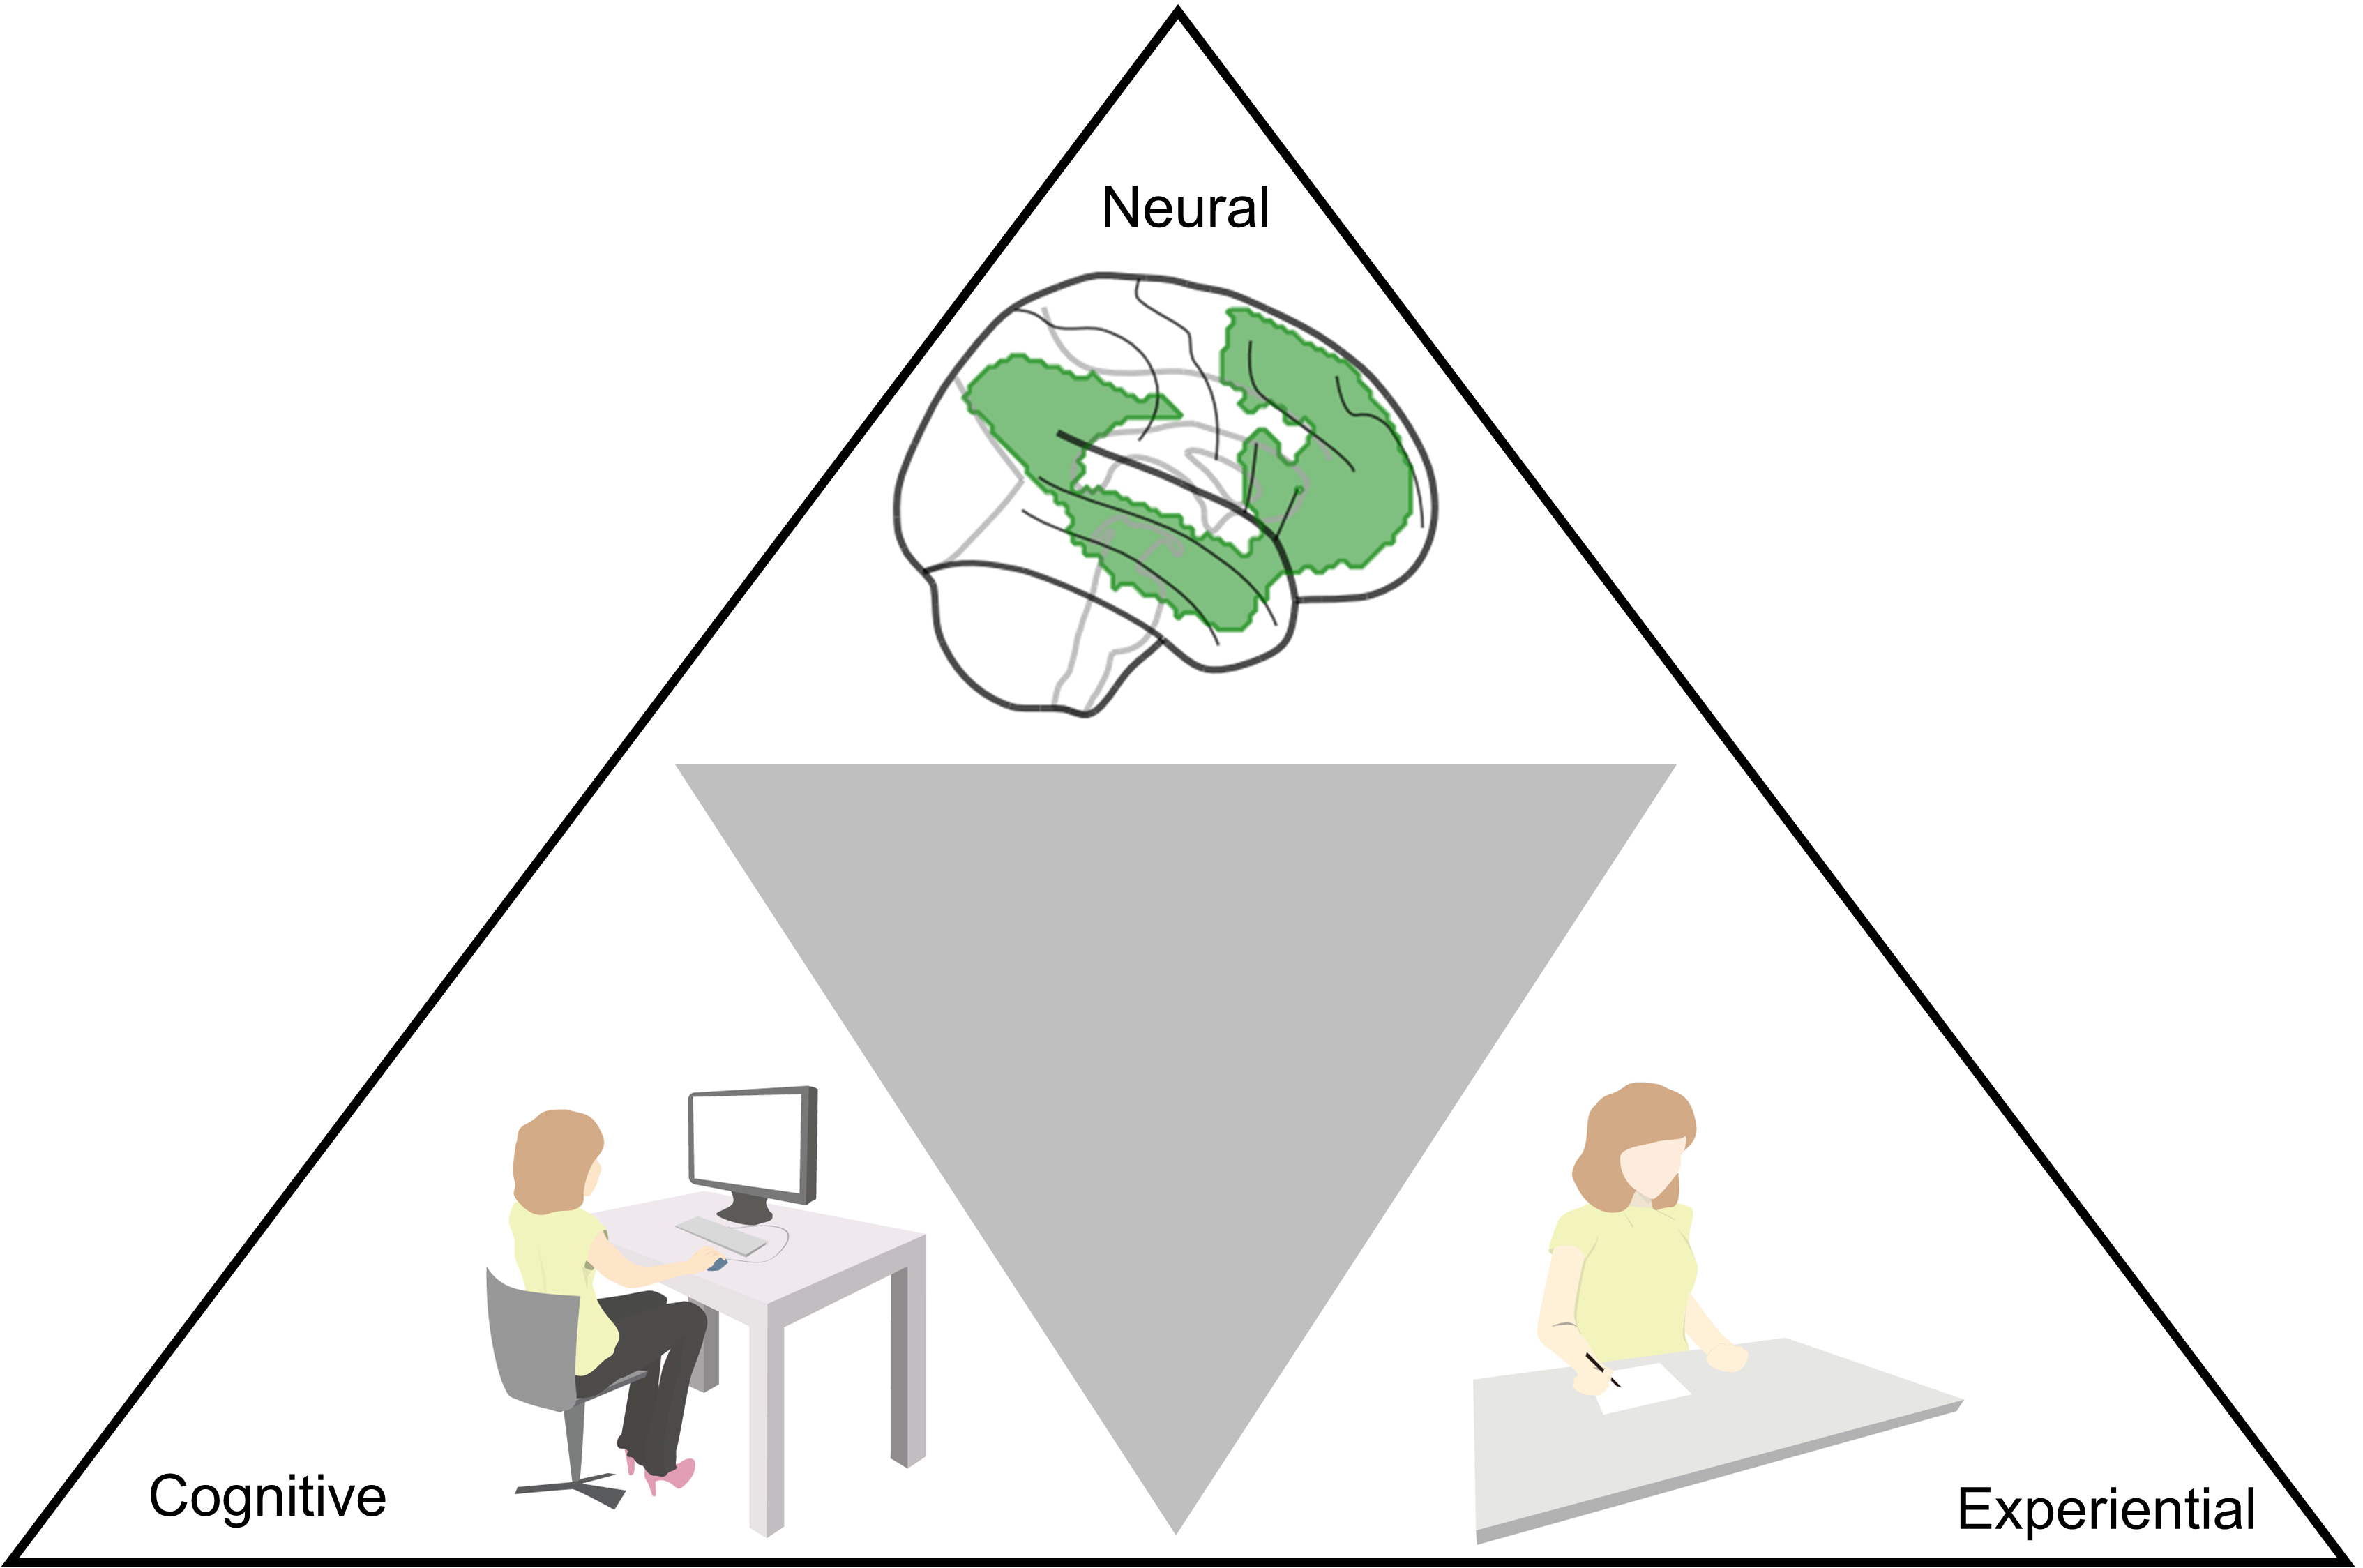
\includegraphics[width=0.8\textwidth]{intro/image/thesisfig1.png}
	\caption{Schematic of the thesis}
	%\vspace{-10pt}
	\label{fig:intro:fig1}
\end{figure}

The current thesis adapts a multivariate approach as the first step towards a new view on mind wandering. Multidimensional experience sampling \cite<MDES; >{Medea2016, RubyPlos2013, Smallwood2016} is the main technique of experience profile assessment. Resting state functional connectivity is used to describe the trait-like neural feature of each individual. The tasks selected measure cognitive functions documented in the past mind wandering literature, including executive control, fluid intelligence, episodic memory, semantic memory, and information generation. Finally, canonical correlation analysis \cite<CCA; >{Hotelling1936} is the conjoined-decomposition method of choice to explore the multivariate patterns of mind wandering. Here I present the overview of the mind wandering measure and the benefit of CCA used in the thesis.  

\subsection{Content of experience}

To access the complex, heterogeneous content of spontaneous thoughts, the current thesis employs MDES \cite{Medea2016, RubyPlos2013, Smallwood2016}. For the purpose of capturing momentary evolution of thoughts during experiments, experience sampling \cite{Kahneman2004} is the commonly used technique. MDES expanded the thought probe from a on/off task question to a collection of dimensions related to a wide range of form and content of thoughts. The idea of MDES is based on various questionnaires to understand the content of mind wandering thoughts retrospectively, such as the Dundee Stress State Questionnaire \cite{Matthews1999}, Amsterdam Resting-State Questionnaire \cite{Diaz2013}, the resting state questionnaire \cite{Delamillieure2010}, and New York Cognition Questionnaire \cite{Gorgolewski2014}. The questionnaires above involves more than 20 items, providing a comprehensive coverage of thought content. Direct implementation of the retrospective questionnaires listed above is not practical for experience sampling. Experience sampling is conducted along an external task, such as reading \cite{Franklin2011}, go/no-go task \cite{Christoff2009}, and n-back task\cite{Kane2007}. The list of questions need to be short and concise to minimum interruption of the external task.

The current version of MDES is based on 10-question set used in \cite{Medea2016} and \citeA{Smallwood2016}. In the previous work, the questions are separated into content and form aspect of experience. Principle component analysis (PCA) was used to extract latent linear structure in the spontaneous thought report. Each participant has a set of identified principle components concluding the average momentary state of all the sampled time period. The current version includes both form and content questions in one set with three extra questions. The average score of each thought dimension indicate the average momentary state of spontaneous thought.

\subsection{Method of acquiring experience}

In the current thesis, both online and retrospective method are used to acquire content of mind wandering in laboratory scenario. In the second empirical study, New York Cognition Questionnaire \cite{Gorgolewski2014} is used to acquire the trait-like multidimensional mind wandering thought content during a 9-minute resting state fMRI session. The retrospective method measures the summary of the mind-wandering experience during a specified time period. The benefit of retrospective measure is that no interruption during the given task or the on-going thoughts will happen. The trait-level features of mind wandering are accessed in the retrospective report. 

In the online measure, MDES serves as the thought probes to record participant's experiences during a give task. Thought probe appears during the task in a semi random fashion. The online measure captures spontaneous thought in, possibly, both mind-wandering and task-focused moments. In the first and third empirical studies, the averaged momentary report from MDES is used to capture the trait-like feature of spontaneous cognition.

% A hybrid of go/no-go task and n-back task was used to manipulate working memory capacity to induce mind wandering \cite{Konishi2015, Medea2016}. The earlier version has used number as the test items \cite{SmallwoodNI2013,SmallwoodPlos2011}. The majority of the experiment consist of nontarget presented in neutral colour and a small proportion of targets. The participant are instructed to judge whether the target number is odd or even. In the \textit{choice reaction time} (i.e. 0-back) condition, the judgement is made when the number changes colour; in the \textit{working memory} (i.e. 1-back) condition, participants judge the number on the previous screen when presented with a question mark. The improved version is proposed by Konishi and colleagues \citeyear{Konishi2015}, replacing number with two 2-dimensional geometric shapes separated by a vertical line. Each pair consists of a two shapes among a circle, a triangle, and a square, each in two different left/right configurations. In the 0-back condition, the target is flanked by one of two shapes, and participants indicate which shape matches the target shape. In the 1-back condition, the target is flanked by two question marks, and participants match the target shape to the prior trial. 

\subsection{Conjoined decomposition of brain and cognition}

Despite invented in the 30s, CCA has not aroused researchers’ interests due to the lack of practicality. With the advance on computing resource and enriched data size, CCA has gained popularity in neuroimaging research. Three characteristic of CCA make it the choice of method---joint information compression, symmetry, and multiplicity (details described in the Method chapter). CCA can be understood as a natural extension of PCA to two variable sets, but mutually linked by a joint correlation criterion. Such extension enables the exploration of neuro-experiential component pairs of mind wandering. CCA does not distinguish between the two variable sets during the information compression process. The identified dual-component dimensions correlates two aspect the data together without indication of causality between neural function and cognition. CCA is capable of estimating more than one corresponding component pair from the two variable sets. More than one pair of meaningful decomposition can be found, giving it the potential to examine the heterogeneity of mind wandering content and their functional outcome. 

While CCA provided useful features to explore the heterogeneity of mind wandering, its sparsity variation overcomes two technical issues of CCA application. Performing feature selection with sparsity improve the interpretability of the data and model fit. The data with more number of features than samples is accompanied with consequences of the so-called curse of dimensionality---the more dimensions are added to a data set, the less explanatory value a sample would have \cite{Domingos2012}. The number of functional connectivity measure can easily exceed the number of samples. In sum, SCCA allows decomposition on functional connectivity measures without sacrifice of data richness or interpretation difficulty of prior data compression. The pros and cons of CCA and its variation is disccussed in the next chapter.

The current thesis adopt the sparse variation of CCA \cite<SCCA; >{WittenSCCA2009} to resolve arguments related to heterogeneity in mind wandering. Most studies in mind wandering have only focused on its relationship with one cognitive outcome at a time. As a consequence, mind wandering is treated as a singular construct. Studies on contents of spontaneous thoughts have shown the diversity of information using self-report methods. Based on the heterogeneity of content of spontaneous thoughts, mind wandering can be a collection various type of spontaneous thoughts. Adopting multivariate method has the potential to identify family resemblance among the heterogeneity of mind wandering, and to begin the research on the ontological view of mind wandering. 

% ==========================================================================================================
\section{Summary and thesis outline}
\sectionmark{Summary}
The mind wandering is a common human experience. Human cognition has the capacity to generate thoughts loosely related to the external world. However, researchers have not understood the mechanism behind the consequences of mind wandering. The heterogeneity of functional outcomes has been a controversial and much disputed subject within the field of mind wandering research. Extensive research has shown that both cost and benefit to cognitive functions are associated with mind wandering. Negative consequences include reduced attention, poor task performance, unhappiness, and depression.  The related positive outcomes include creative problem solving, planning personal goals, and recovery from negative emotion. 

Most studies in mind wandering have only focused on one cognitive outcome at a time. Mind wandering is treated as a singular construct. Studies on contents of spontaneous thoughts have shown the diversity of information using self-report methods.  The temporal content of spontaneous thoughts can be future- or past-focused. The topic can be on personal issues or task related. Based on the heterogeneity of content of spontaneous thoughts, mind wandering can be a collection various type of spontaneous thoughts. The lack of specificity in thought content could result in conflicts in the functional outcome of mind wandering literature.

In the past decade, the neural basis of mind wandering has become the centre of the topic. DMN is the commonly emerged large-scale network. Extensive literature have documented the task-negative trait of DMN. The executive failure account of mind wandering is in line with the task-negative view of DMN. However, the memory representation aspect of the mind wandering mystery is left unresolved. Recent literature on the neural hierarchy has shade a different light on the function of DMN. The high-level cognitive functions are associated with DMN, whereas perception and motor related regions are related to low-level tasks. This new view provides a clue to investigate the representational account of mind wandering. 

The conflict in mind wandering literature is related to the one-to-one matching between mind wandering and the brain or behaviour. To paint the full picture of mind wandering, a multivaritate method will help incorporate the three aspects mentioned above: cognition, experience, and neural basis. The current thesis adopt CCA to resolve arguments related to heterogeneity in mind wandering. Despite invented in the 30s, CCA has not aroused researchers’ interests due to the lack of practicality. With the advance on computing resource and enriched data size, CCA has gained popularity in neural imaging research. The motivation of the current thesis is to resolve the conflict in mind wandering literature incorporating functional organisation of large-scale neural networks. The aim is to present evidence supporting the heterogeneity of mind wandering and to begin research on the ontological view of mind wandering. A outline of the remaining chapter is listed below: 

\subsection*{Canonical correlation analysis}

Canonical correlation analysis is introduced as the main method of the thesis. This review focuses the potential applications in neuroimaging research. The features, applications of this multivariate method are outlined, followed by discussion on the method's the interpretations and limitations. 

\textit{This chapter is under preparation for publication. } 

\subsection*{Exploring the heterogeneity of on-going thought}
Heterogeneity of mind wandering leads to conflicts in its functional outcome in behavioural study. Default mode network is commonly associated with the emergence of mind wandering. Sparse CCA conjointly decomposed functional connectivity patterns of DMN and thought reports, revealing unique neuro-experiential components. The study then revealed that the neuro-experiential components each associate with unique cognitive task measures. The various connectivity configuration within DMN is associated with different types of mind wandering and their specific functional outcomes.

\textit{This chapter is published in Psychological Science.}

\subsection*{Population variation in the associations between large-scale network and experiences}
Unconstrained cognitive processes have two faces. The representational account argues that the primary sensory brain region decoupling from the DMN to facilitate memory representation; whereas the executive failure account shows lapses in attention is related to the demand to attention system and activation of DMN. Mind wandering is an unconstrained cognitive state, therefore we used sparse CCA to extract related whole brain functional connectivity patterns, profiling the neuro-experiential components of unconstrained cognitive processes. Examining the association between demanding cognitive tasks and neuro-experiential components, the study revealed evidence supporting both the representational and executive failure accounts.

\textit{This chapter is published in NeuroImage.}

\subsection*{Inhibition of prior information contributes to internal content representation}
Various cognitive function is involved in the generation of internal experiences. The study of the functional outcome are often conducted in a manner of one-to-one mapping. The heterogeneous cognitive outcomes are discussed as conflicts rather than the complex details driving the diversity of mind wandering. In the current chapter, we explore the intrinsic whole-brain neural basis of the cognitive functions supporting the unconstrained generation of spontaneous thoughts.  With sparse CCA we describe the conjoined decomposition of cognitive function and resting state functional connectivity. The study explore the unconstrained neruocognitive mechanism underlying the various dimensions of spontaneous thoughts.

\subsection*{General discussions}
The overarching themes of the thesis are discussed and linked to specific results throughout the thesis. Future research directions are inspired by the findings and limitations of the current thesis.

% ==========================================================================================================

\chapter{Canonical Correlation Analysis}
\label{ch:methods}

%\setcounter{equation}{0}
% ==========================================================================================================

\textit{The following chapter has been adapted from:}
Wang, H.-T., Smallwood, J., Satterthwaite, T. D., Bassett, D. S., \& Bzdok, D. (2018). Finding the needle in high dimensions: A tutorial on CCA in biomedicine. Manuscript preparing for publication.
\footnote{D. Bzdok and H.-T. Wang planned the structure of the manuscript.  H.-T. Wang. drafted the manuscript under the supervision of D. Bzdok and J. Smallwood.}
% ==========================================================================================================
\section{Abstract}

Since the beginning of the \nth{21} century, the sample size of studies in medicine and neuroscience has grown rapidly. For example data sets with thousands of subjects are common and they often entail extensive neural and behavioural phenotyping yielding datasets with tens of thousands of variables. The size and complexity of these big data sets pose new challenges to researchers hoping to use them to understand relationships between brain, cognition and disease. Canonical correlation analysis (CCA) is a promising method for dealing with these large data sets. CCA allows two or more source of information to be simultaneously evaluated, such as descriptions of the brain and behaviour. The present tutorial paper describes the rationale for using CCA, and considers both the promises, and pitfalls of this technique in the field of cognitive neuroscience.

% ==========================================================================================================

\section{Motivation}
\label{ch:methods:motivation}
Massive biomedical datasets and increasing computational power are opening the door to a new regime of data analysis. Similar to the advent of micro-arrays in genetics, brain-imaging and extensive behavioural phenotyping yield datasets with tens of thousands of variables. In the beginning of the 21st  century, the sample size of studies in medicine and neuroscience started to grow rapidly \cite{Efron2010Book}. Popularity of non-invasive brain-imaging methods provided convenient measure of brain activity and more measurement units per subject than considered participants. The advance in psychological science increased granularity of behavioural phenotype and demographic information. For instance, UK Biobank is a prospective population study with 500,000 participants and comprehensive imaging data, genetic information and environmental measures on mental disorders and other diseases \cite{AllenUKBioBank2012,MillerR2016}. %ukbiobank
The Human Connectome Project \cite<HCP; >{VanEssen2013} has recently completed brain-imaging of more $>$10,000 young adults, with 4 hours of scanning per subject, and utilising vast improvements in the spatial and temporal resolutions of the acquired data. The Cambridge Centre for Ageing and Neuroscience \cite<Cam-Can; >{Taylor2017,Shafto2014} a large ($N >= 700$), cross-sectional adult lifespan (18--87 years old) population-based sample designed to characterise age-related changes in cognition and brain structure and function, with raw and preprocessed brain imaging data and cognitive behavioural experiments and demographic and neuropsychological data. Extensive phenotype and big sample size do not provide benefits without costs. Many classical statistical tools struggle to resolve datasets with more variables than observations. Moreover, the increasing data richness is accompanied with less explanatory value of a sample. The growing interest in big datasets will soon motivate researchers to seek alternative tools to ask and answer research questions in challenging rich data. 

Many classical linear-regression approaches have much contributed in the advance of neuroimaging. However, high-dimensional data were not taken into consideration when classic linear models initially designed. The present tutorial paper introduces rationale, promises, and pitfalls of one promising analysis strategy: Canonical correlation analysis (CCA). The key feature of CCA is simultaneous evaluation of two sources of detailed information, such as many brain measurements and many behavioral measurements. Two large variable sets are simultaneously co-analyzed with the capability of CCA to identify the main directions of variation in the data. CCA is an early example of multivariate statistical methods introduced in 1936 \cite{Hotelling1936}. However, the application of CCA has long been dormant largely due to insufficient computation power and data size. The issues once hindered the practical application of CCA were overcame, resulting in the revival of CCA in 21st century biomedicine. CCA aims not only to decompose the data into hidden sources of variation but also the correspondence between linked dimensions of two sets of variables. The possible relations between essential information from two variable sets (ie. brain and behavior) may be better reflected by the doubly-multivariate decomposition character of CCA.  In imaging and genetic neuroscience, cognition or brain function can be studied by capturing variability which does not come to the surface in a one-to-one (e.g., Pearson's correlation) or many-to-one (e.g., linear support vector machines) mapping approach. With CCA's conjoined decomposition on two variable sets, researchers can examine the hidden linear structure among various diverse variables. CCA has the capacity to yield sets of linked dimensions that explain a series of observations. The paired dimensions provide alternative views on the relations among variables. With substantially larger set of measurements and the pursuit of complex research questions, researchers in neuroscience have gained increasing interests in CCA. CCA has proven be inspirational methodology for new and continuing research \cite{Marquand2017, Smith2015,Tsvetanov2016,VatanseverNI2017,WangPsychScience2018,WangPsychScience2018} with its ability to reduce the data to meaningful and concise information that allows the original experimental question to be answered. 

Our guide to CCA proceeds in four parts. We first introduce the model in details and the circumstances of use with recent applications of CCA in existing research. Next, we detail the interpretation spectrum of the CCA algorithm including limitation and pitfalls of CCA, and its similarity to other modeling technique. In closing, we provide practical suggestions of analysis.

% ==========================================================================================================
\newpage
\begin{infobox}{CCA and general linear model (GLM)}
CCA can be framed as a general example of other statistical procedures that are derived from the general linear model (GLM). Virtually all of the parametric tests most often used by behavioral scientists (e.g., ANOVA, MANOVA, multiple regression, Pearson correlation, t-test) can be subsumed by CCA as special cases in the GLM (Knapp, 1978; Thompson, 2010). Because these techniques are intricately related and fundamentally the same in many respects of CCA, learning CCA may help facilitate conceptual understanding of statistical methods throughout the GLM.
\end{infobox}

\section{Modelling intuitions}
\label{ch:methods:intuitions}
One way to appreciate the idea behind CCA is by viewing this procedure as an extension of the widely applied principle component analysis (PCA)(See Box 2.1). A principle component finds the hidden information sources that describe the biggest sources of variation among the variables. A close approximation of the original data can be reconstructed by the hidden variance source. In other words, PCA converts a set of correlated variables into a smaller number of hidden factors that were not directly observable in the original data, but effectively explain the structure of particular observation. As a prominent example, the big five personality is a psychological construct of human personality traits discovered through PCA. Personality survey data entered PCA and then finds the five hidden components that explains most of the meaningful variance of the data. The advantage of decomposition method such as PCA is its ability to reduce the original datasets to fewer and thus more interpretable dimensions. Such re-expression of the original data in a compressed, more parsimonious form has computational-statistical and interpretational appeal, while still capturing a large amount of the variability in the original large variable array. CCA maximizes the linear correspondence between linear combinations of two variable sets, similar to carrying out two PCA decompositions, but mutually linked by a joint correlation criterion. CCA reveal the two linear models describing the hidden structures. The generating process is mutually constrained by the maximum correlation of the hidden structures. Such extension of the traditional hidden factor approaches enables two sets of measurements, for example, i) genetics and behavior, ii) brain and behavior, or iii) brain and genetics. Three aspects together are characteristic for modeling data using CCA:


\begin{figure}[H]
    \vspace{-10pt}
    \centering
    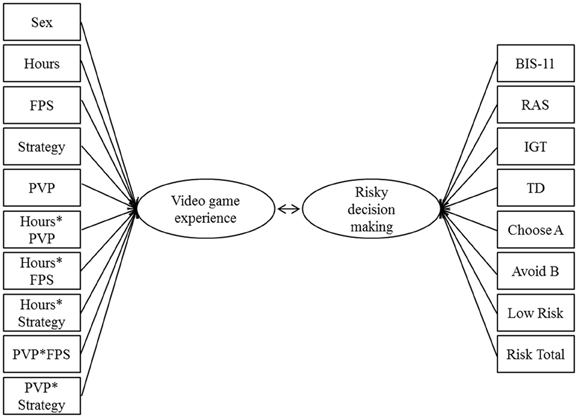
\includegraphics[width=0.8\textwidth]{cca/image/ccafig1.jpg}
	\caption{An example of CCA on behavioural data.}
	\linespacesmall
	\footnotesize
	\caption*{\cite{Bailey2013}. Consider a case of exploring the relations between movie genre and personality with CCA. On the left hand side, we can input the data related to movies the participants watched, such as number of action / documentary / comedy etc. movies watched. The right hand side is the personality rating of the participants, for example extrovert vs not, openness vs not etc. The CCA can then find the related personality traits with the type of movies they are likely to watch.}
    \linespacenormal
	\label{fig:methods:fig1}
	\vspace{-20pt}
\end{figure}


\subsection{Joint information compression}
The purpose of CCA is finding variability components hidden in each of two variables sets.  The linear relations of the variable sets are determined when the variation in strength of involvement across subjects is maximally correlated. The relations to a pair of factors, their canonical correlations, indicates the conjoined explained variance across both information reductions. In a similar manner of PCA, the variables summarized the original high-dimensional variable sets with a pair of linear relations. The linear re-expression summarizes aspects of the data-generating process that was mutually constrained by the sets of input variables. The canonical correlation determines the joint explanatory power shared in the two input variable sets. CCA aims to find the most compact decomposition based on the variance explained under the contained of uncorrelated hidden dimensions. The more important components will be discovered in the earlier order.

\subsection{Symmetry}
CCA does not distinguish between the left and right variable sets during the information compression process. The canonical correlation indicates that a unit change in one component is consistently associated with an equivalent change in another component. Therefore, numerically identical decomposition results are returned regardless of the input order of two variable sets. Symmetry is a key feature that distinguish CCA from other linear regression methods. In linear-regression models, dependent and independent variables play diverging roles in the analysis. Regression indicate the impact of a unit change in the independent variable on the dependent variables, therefore dependent and independent variables cannot be exchanged to obtain an identical result. CCA, as a correlation based method, describes the co-relationship of the two variable sets, thus the exchange of the two variable sets produces identical results.

\subsection{Multiplicity}
CCA can estimating more than one corresponding component pair from the two variable sets. A pair of the components forms a mode. After finding the most important mode, CCA would then determine the subsequent linear combinations in the data patters that remain to be explained in addition to the already extracted factors. Since every new identified mode was found in the unexplained variance to the preceding mode, the modes are optimized to be uncorrelated to each other. In this manner, CCA produces a set of mutually orthogonal modes naturally ranked by explained variance. The orthogonality constraint ensues the modes each representing unique linear patterns that dominate different features in the data. When the modes are meaningful to the theory, the researchers can potentially formulate a component process approach to interpret the data.

In this way, CCA uncovers effective, symmetric linear relations that compactly summarize doubly-multivariate data. We introduced three important characteristics of CCA. First, CCA provides more effective hidden representation that capture most variance in original variables. Next, the CCA model is symmetrical in the sense that no numerical difference happens in the exchange of the two variable sets. Finally, we can estimate several modes of correspondence between the two variable sets. In the next section, we would like to explore examples of CCA applications.


\subsection{Examples}
Smith and colleague (Smith et al., 2015; see Figure 2 for the analysis pipeline) employed CCA to uncover brain-behavior modes of population co-variation in the Human Connectome Project (HCP; van Essen et al., 2013). \citeA{Smith2015} aimed to discover whether any specific patterns of functional brain connectivity, on the one hand, are associated with specific sets of correlated demographics and behaviour on the other hand. Functional brain connectivity was retrieved from resting state functional scans. The resting state scans measure the brain activity in the absence of a task or stimulus. 200 independent component analysis (ICA; Beckmann, Mackay, Filippini, \& Smith, 2009) networks were obtained from the resting state scans. ICA identifies all the independent networks by separating the spatial sources of the resting state data. The functional connectivity matrices were calculated based on the pair-wise correlation of the 200 networks. The behavioral measures ranging from cognitive function to demographic information entered the CCA along the functional connectivity matrices. The robustness of the modes were accessed via permutation tests on the canonical correlation. One significant mode demonstrated strong population level co-variation of network connectivity and behavioural measures. The behavioural measures spread along a positive-negative axis with intelligent, memory and cognition tests and life-satisfactory on the positive end and negative life-style measures anchoring the other end. The brain regions highly contributing to the connectivity resembles the default mode network  (DMN; Buckner, Andrews-Hanna, \& Schacter, 2008) . The positive-negative dimensions in the behavioural component and the emergence of DMN in the brain component may seem trivial on their own, however, CCA formalised the relation of the underlying biology and the correlation among the general behavioural measures that captures intelligence. Regions composing DMN has been associated with episodic and semantic memory, scene construction, and complex social reasoning such as theory of mind. The finding of Smith and colleagues (2015) strengthen the relation between DMN and high-level cognition, especially intelligence - one of the perhaps most important indices so far identified in by psychologists.

\begin{figure}[H]
	\centering
	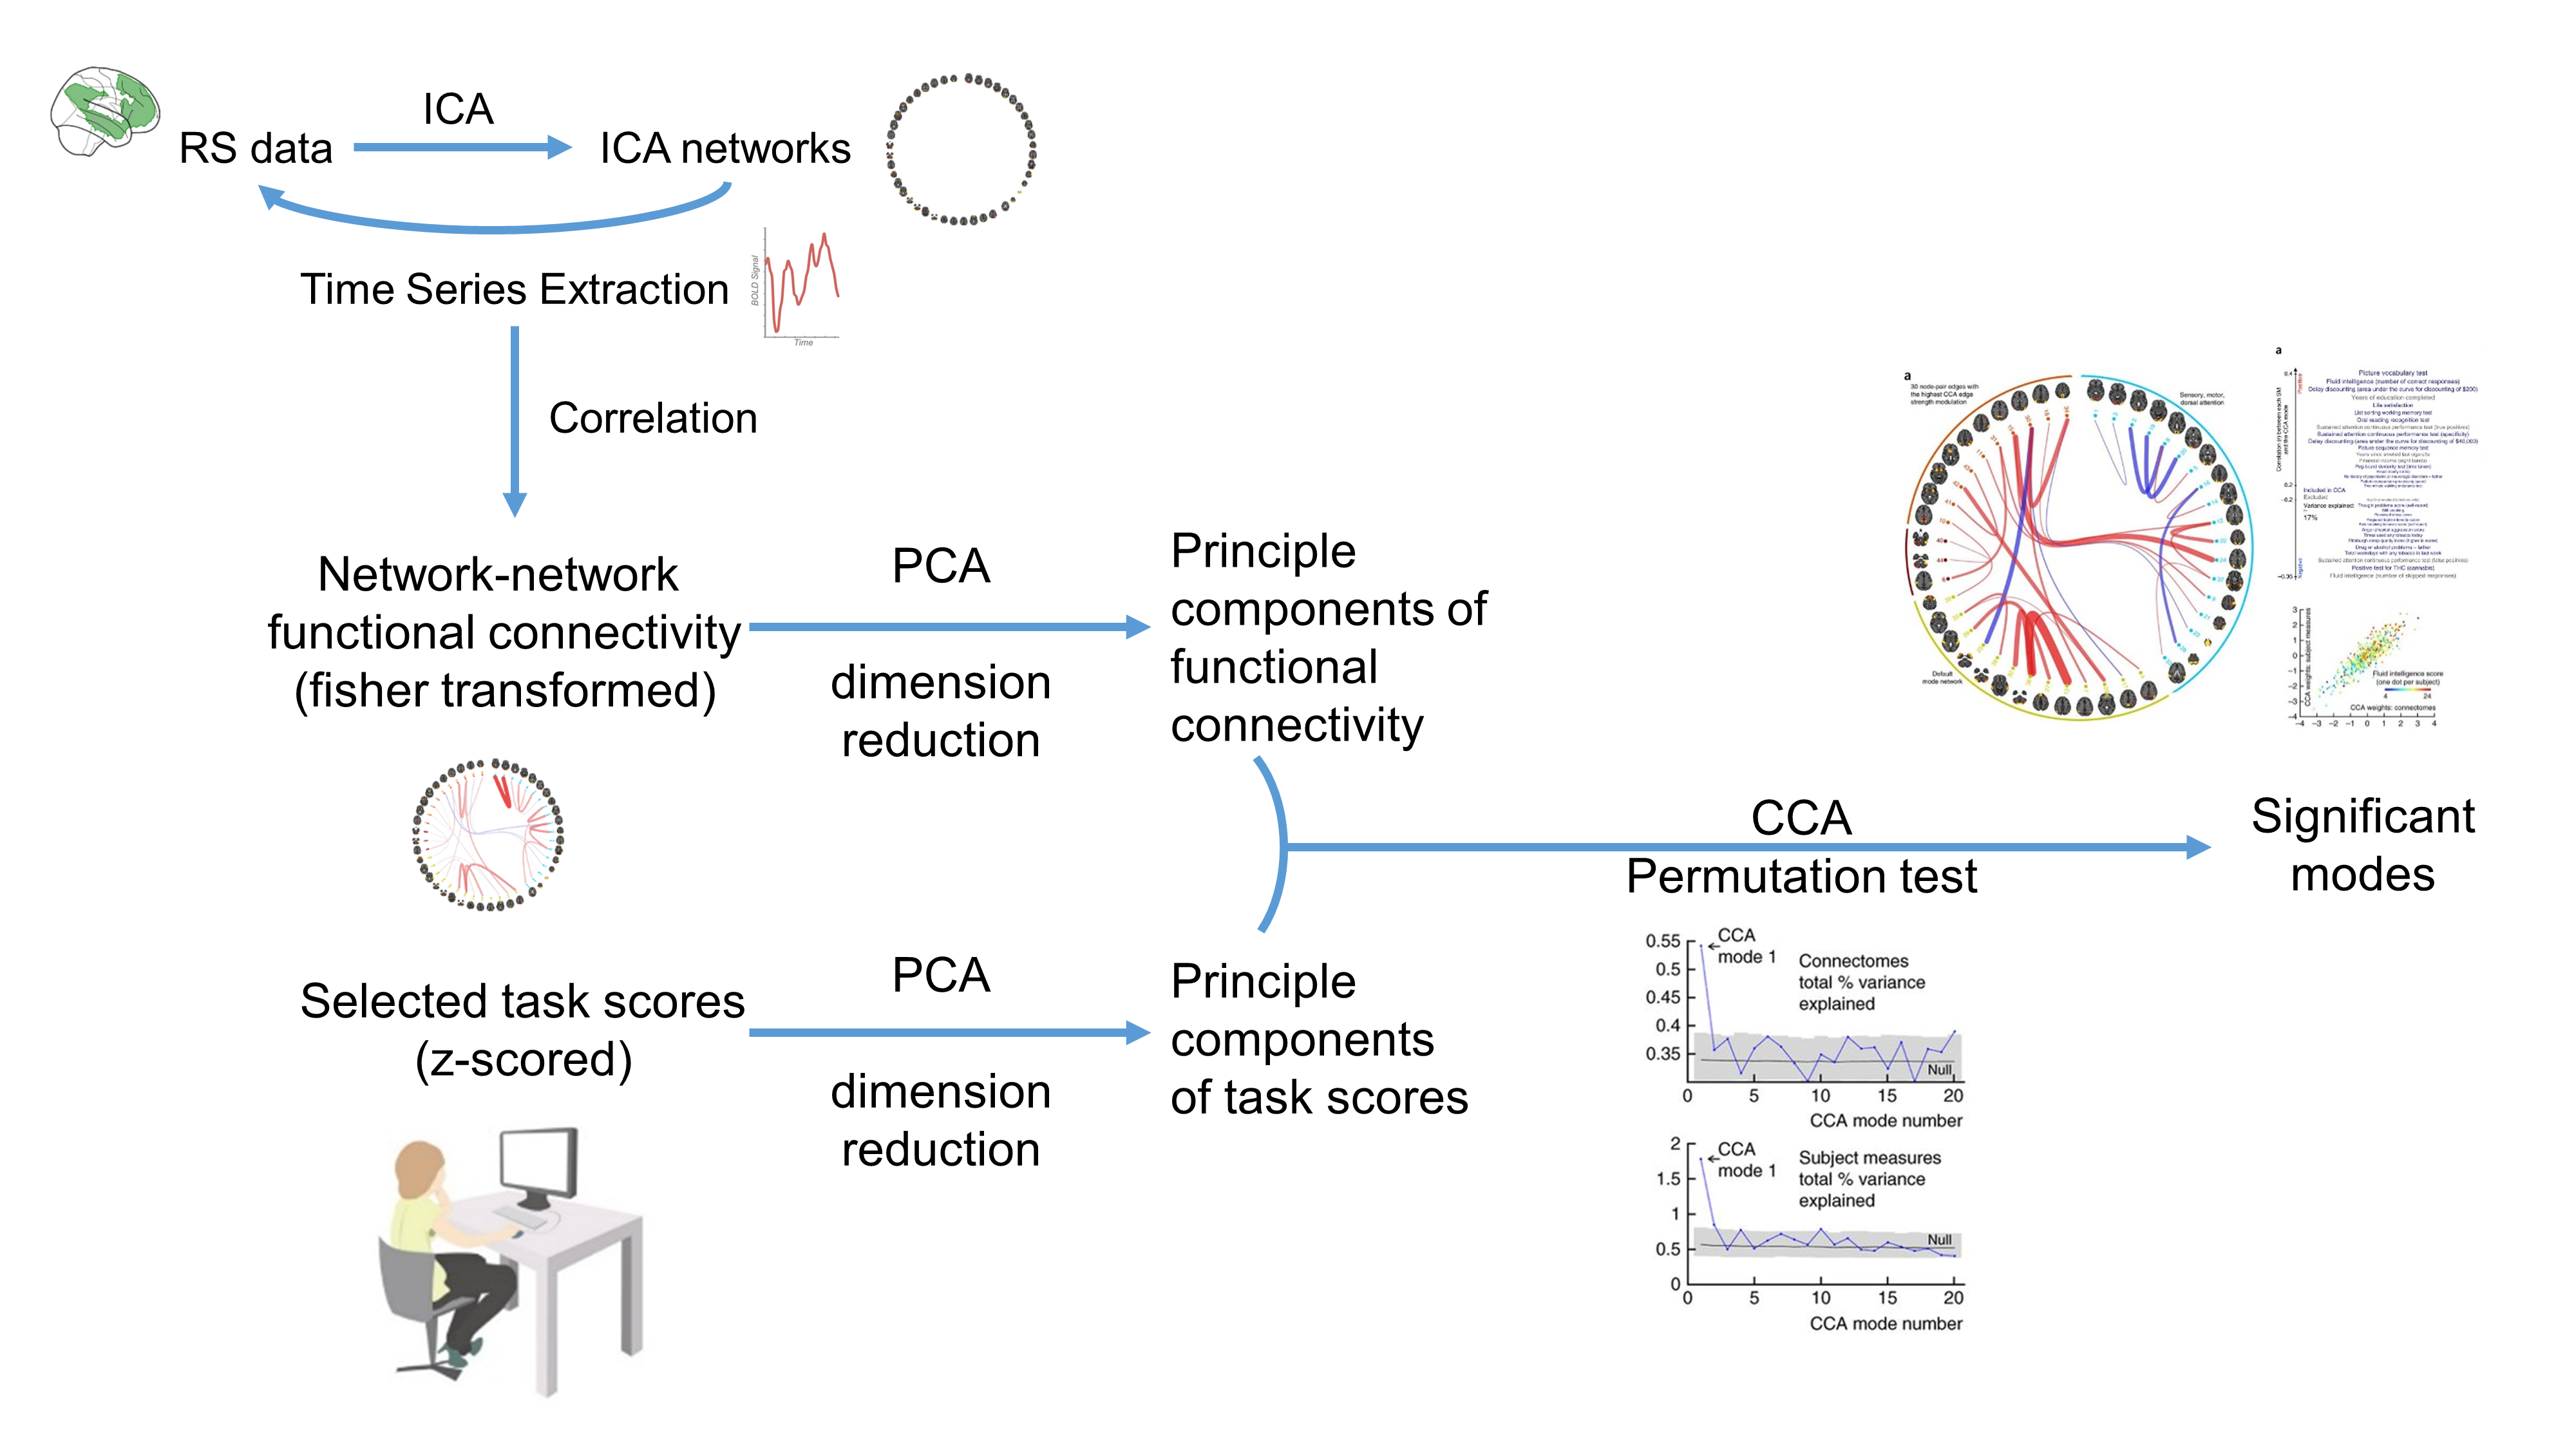
\includegraphics[width=1\textwidth]{cca/image/ccafig2.png}
	\caption{The analysis pipeline of Smith et al. (2015). The arrows represent analysis performed.}

	\label{fig:methods:fig2}
\end{figure}

Wang and colleagues (Wang et al., 2018; see Figure 3 for the analysis pipeline) uncover the relation between DMN and mind wandering. Mind wandering is associated with poorer performance on attention demanding tasks (McVay \& Kane, 2009; Mrazek et al., 2012), yet studies of problem solving suggest that mind wandering may promote creativity (Baird et al., 2012; Smeekens \& Kane, 2016). Despite the heterogeneity of functional outcomes, task-unrelated thoughts during mind wandering are linked to concurrent increases in DMN activity (see review from Smallwood \& Schooler, 2015). DMN is most commonly known as a task-negative network (Fox et al., 2005); however, emerging evidences suggested DMN’s role in information integration (Margulies et al., 2016). This study further explored whether the different within-DMN activation patterns underlie different types of mind wandering thought, resulting in conflicting associations to cognitive function in the mind-wandering literatures. The connectivity among 16 DMN regions and 13 self-report questions on thoughts entered the sparse variation of CCA (Witten, Tibshirani, \& Hastie, 2009). Two stable modes corresponded to traits of positive-habitual thoughts and spontaneous task-unrelated thoughts with different neural connectivity patterns in the DMN. The modes were uniquely related to aspects of cognition, such as executive control and the ability to generate information in a creative fashion, and independently distinguished well-being measures. The conflicted mind-wandering related executive failure and creativity related benefits was resolved including neural data in spontaneous thoughts decomposition. Wang and colleagues (Wang et al., 2018) showed that mind wandering is a collective term for various types of spontaneous thought. Different brain instantiations located in the DMN is the key to identify different types of spontaneous thought. The different configurations of DMN also demonstrated its possible role as an integrator in cognition, rather than a task-unrelated network.

\begin{figure}[H]
	\centering
	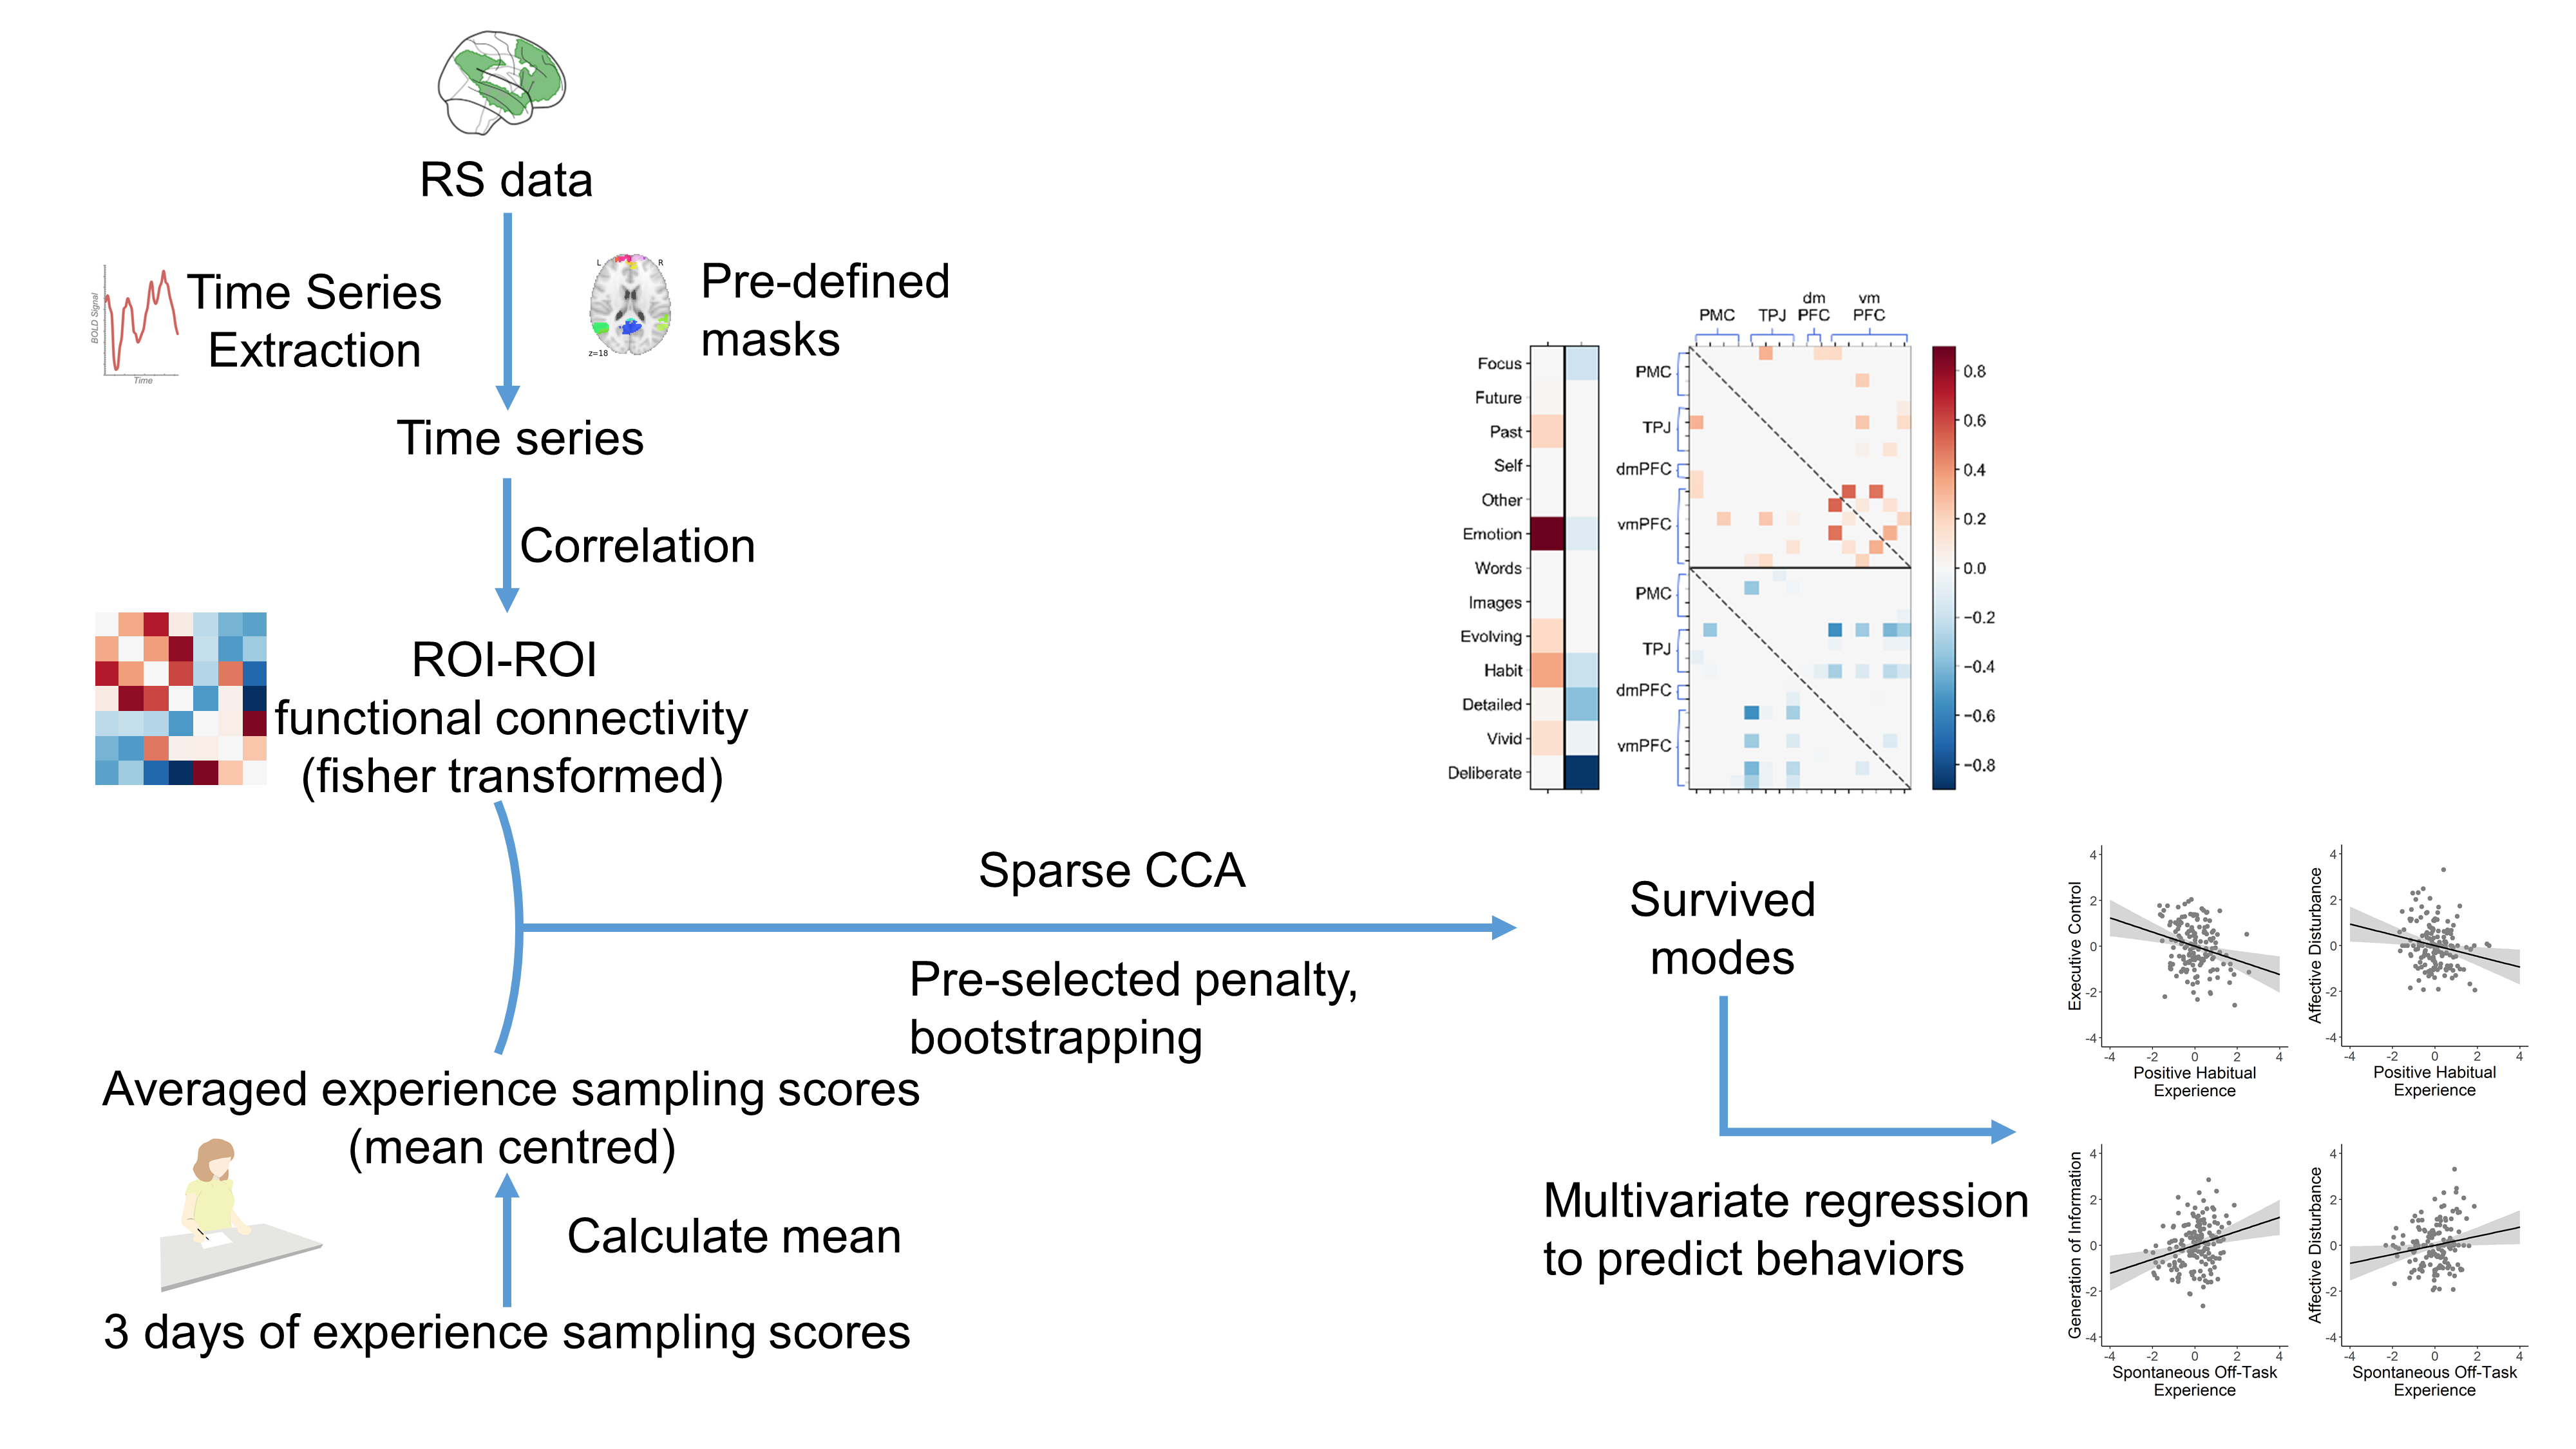
\includegraphics[width=1\textwidth]{cca/image/ccafig3.png}
	\caption{The analysis pipeline of WangPsychScience2018. The arrows represent analysis performed.}

	\label{fig:methods:fig3}
\end{figure}

% ==========================================================================================================

\begin{infobox}{CCA and related linear methods}

CCA is related to other feature learning methods in neuroscience. As mentioned in the modelling intuition section, \textbf{PCA} is a similar method performed on one set of variables only. The objective of PCA is a transformation of several possibly correlated variables into a smaller number of uncorrelated variables known as principal components. PCA compresses data into a smaller number of factors that carries most of the variance of the data.

\textbf{Independent component analysis} (ICA) to perform a linear transform that makes the resulting variables as statistically independent from each other as possible. The basic assumption behind ICA is that the data is composed of independent source of information. In contrast to PCA and CCA, all components are equally important.  ICA helps when you want to find a representation of your data as independent sub-elements

\textbf{Partial least squares} (PLS) regression and CCA are both techniques for feature extraction from two sets of multidimensional variables. The fundamental difference between CCA and PLS is that CCA maximizes the correlation while PLS maximizes the covariance. PLS is a supervised approach attempts to find directions that help explain both the response and the predictors. Most of the comparison between PLS and CCA are focused on the generation of the first components. There is no one way to compute the other components in PLS (De Bie et al., 2005).
\end{infobox}

\section{Interpretations}
\label{ch:methods:interpretations}
The symmetrical data compression feature of CCA helps researchers to handle the complexity of two variable sets. However, whether the process of the analysis is an exploration of hidden structures or mutually constrained predictive component has been an unsettled debate. CCA can be viewed as a supervised predictive algorithm or as an unsupervised exploratory algorithm. A supervised algorithm relies on the predefined labels/relationships in the data to form prediction; whereas an unsupervised algorithm aims to extract patterns in the data with unlabeled data. CCA has some properties of both supervised and unsupervised modeling approach. Depending on which perspective is adopted, the functions of CCA and the potential interpretation can be very different.  The more the dimensionality of one of the variable sets resembles the single output of linear-regression-type methods, the more CCA application approaches output estimation of a supervised estimator. The larger the variable sets on both sides, the more CCA approaches exploratory pattern discovery.

The main difference between supervised and unsupervised method lays in whether there is a learning target or loss function. In supervised learning, the loss function determines the best parameters to form prediction. The difference between the prediction generated by the model and the real label is the objective of a so-called loss function. CCA has as objective to maximize the linear correlation between the latent dimensions from two variable sets. While most of supervised learning methods estimates loss between real data and predictions, CCA has an unusual objective that we rarely see in supervised estimators.  Symmetry is another reason that makes CCA an unusual case of supervised learning. In supervised learning, the model learns the pattern in the data to predict a set of targets. The symmetrical nature of CCA does not distinguish the two sets of input variables. The data compression and hidden structure inspection aspect puts CCA in line with unsupervised methods. The conjoined decomposition captures the relations among the variables. The found relations are used to construct fewer factors that capture the variance of the original data. CCA has the strength of both supervised and unsupervised methods. Like unsupervised methods, CCA can search through candidate patterns to find structure in data. The accurate predictions formed by CCA highlights the trait of a supervised method. In conclusion, CCA is a special case that sits in-between the supervised and unsupervised methods. The flexibility in interpretation offers people multiple ways to utilize CCA in research.

Statistical methods can be categorized into three categories based on their goals: estimation, prediction, and inference.  Estimation represents ways or a process of learning and determining the population parameter based on the model fitted to the data. Prediction is making inference of an unknown data points based on information obtained from a sample. Inferential statistical analysis utilizes hypothesis testing to draw conclusions about populations or scientific truths from data. CCA falls into the family of estimation. The focus of CCA is to establish statistical associations (i.e. the latent linear relations among variables, the association between the two latent linear relations). Predicting some variables based on other variable is not the optimization goal. CCA does not seek to establish “statistically significant links between variables”. The null hypothesis that is really tested around the robustness of the latent space correlation (i.e., the canonical correlations of the latent variables extracted from the two variable sets) across modes, not so much particular variable-variable links. CCA is often used to rigorously evaluate whether overall linked covariation patterns can be found in two variable sets, rather than pinpointing and “putting the finger on” certain specific relations that should be interpreted with more caution.

% ==========================================================================================================
\subsection{Utility of CCA}
\label{ch:methods:limitations}
The strength and benefit of CCA do not come without limitations. Here we discuss several aspects the researchers should keep in mind when evaluating whether the data set is suitable for CCA. CCA can handle data with more observations than number of variables of the smaller variable set (i.e. $p < min(m, n)$). However, smaller dataset does not fully utilise the strength of CCA in concluding the variability in data. Research areas like neuroscience often look into small effect magnitude in correlation, thus a larger sample size is required to correctly infer the variability in data. On the other hand, if the number of variables of either side of the equation exceeds the sample size, CCA does not generate unique linear combinations for each variable set. In such scenario, a PCA rank-reduction preprocessing step is commonly performed before applying CCA.

\begin{figure}[H]
	\centering
	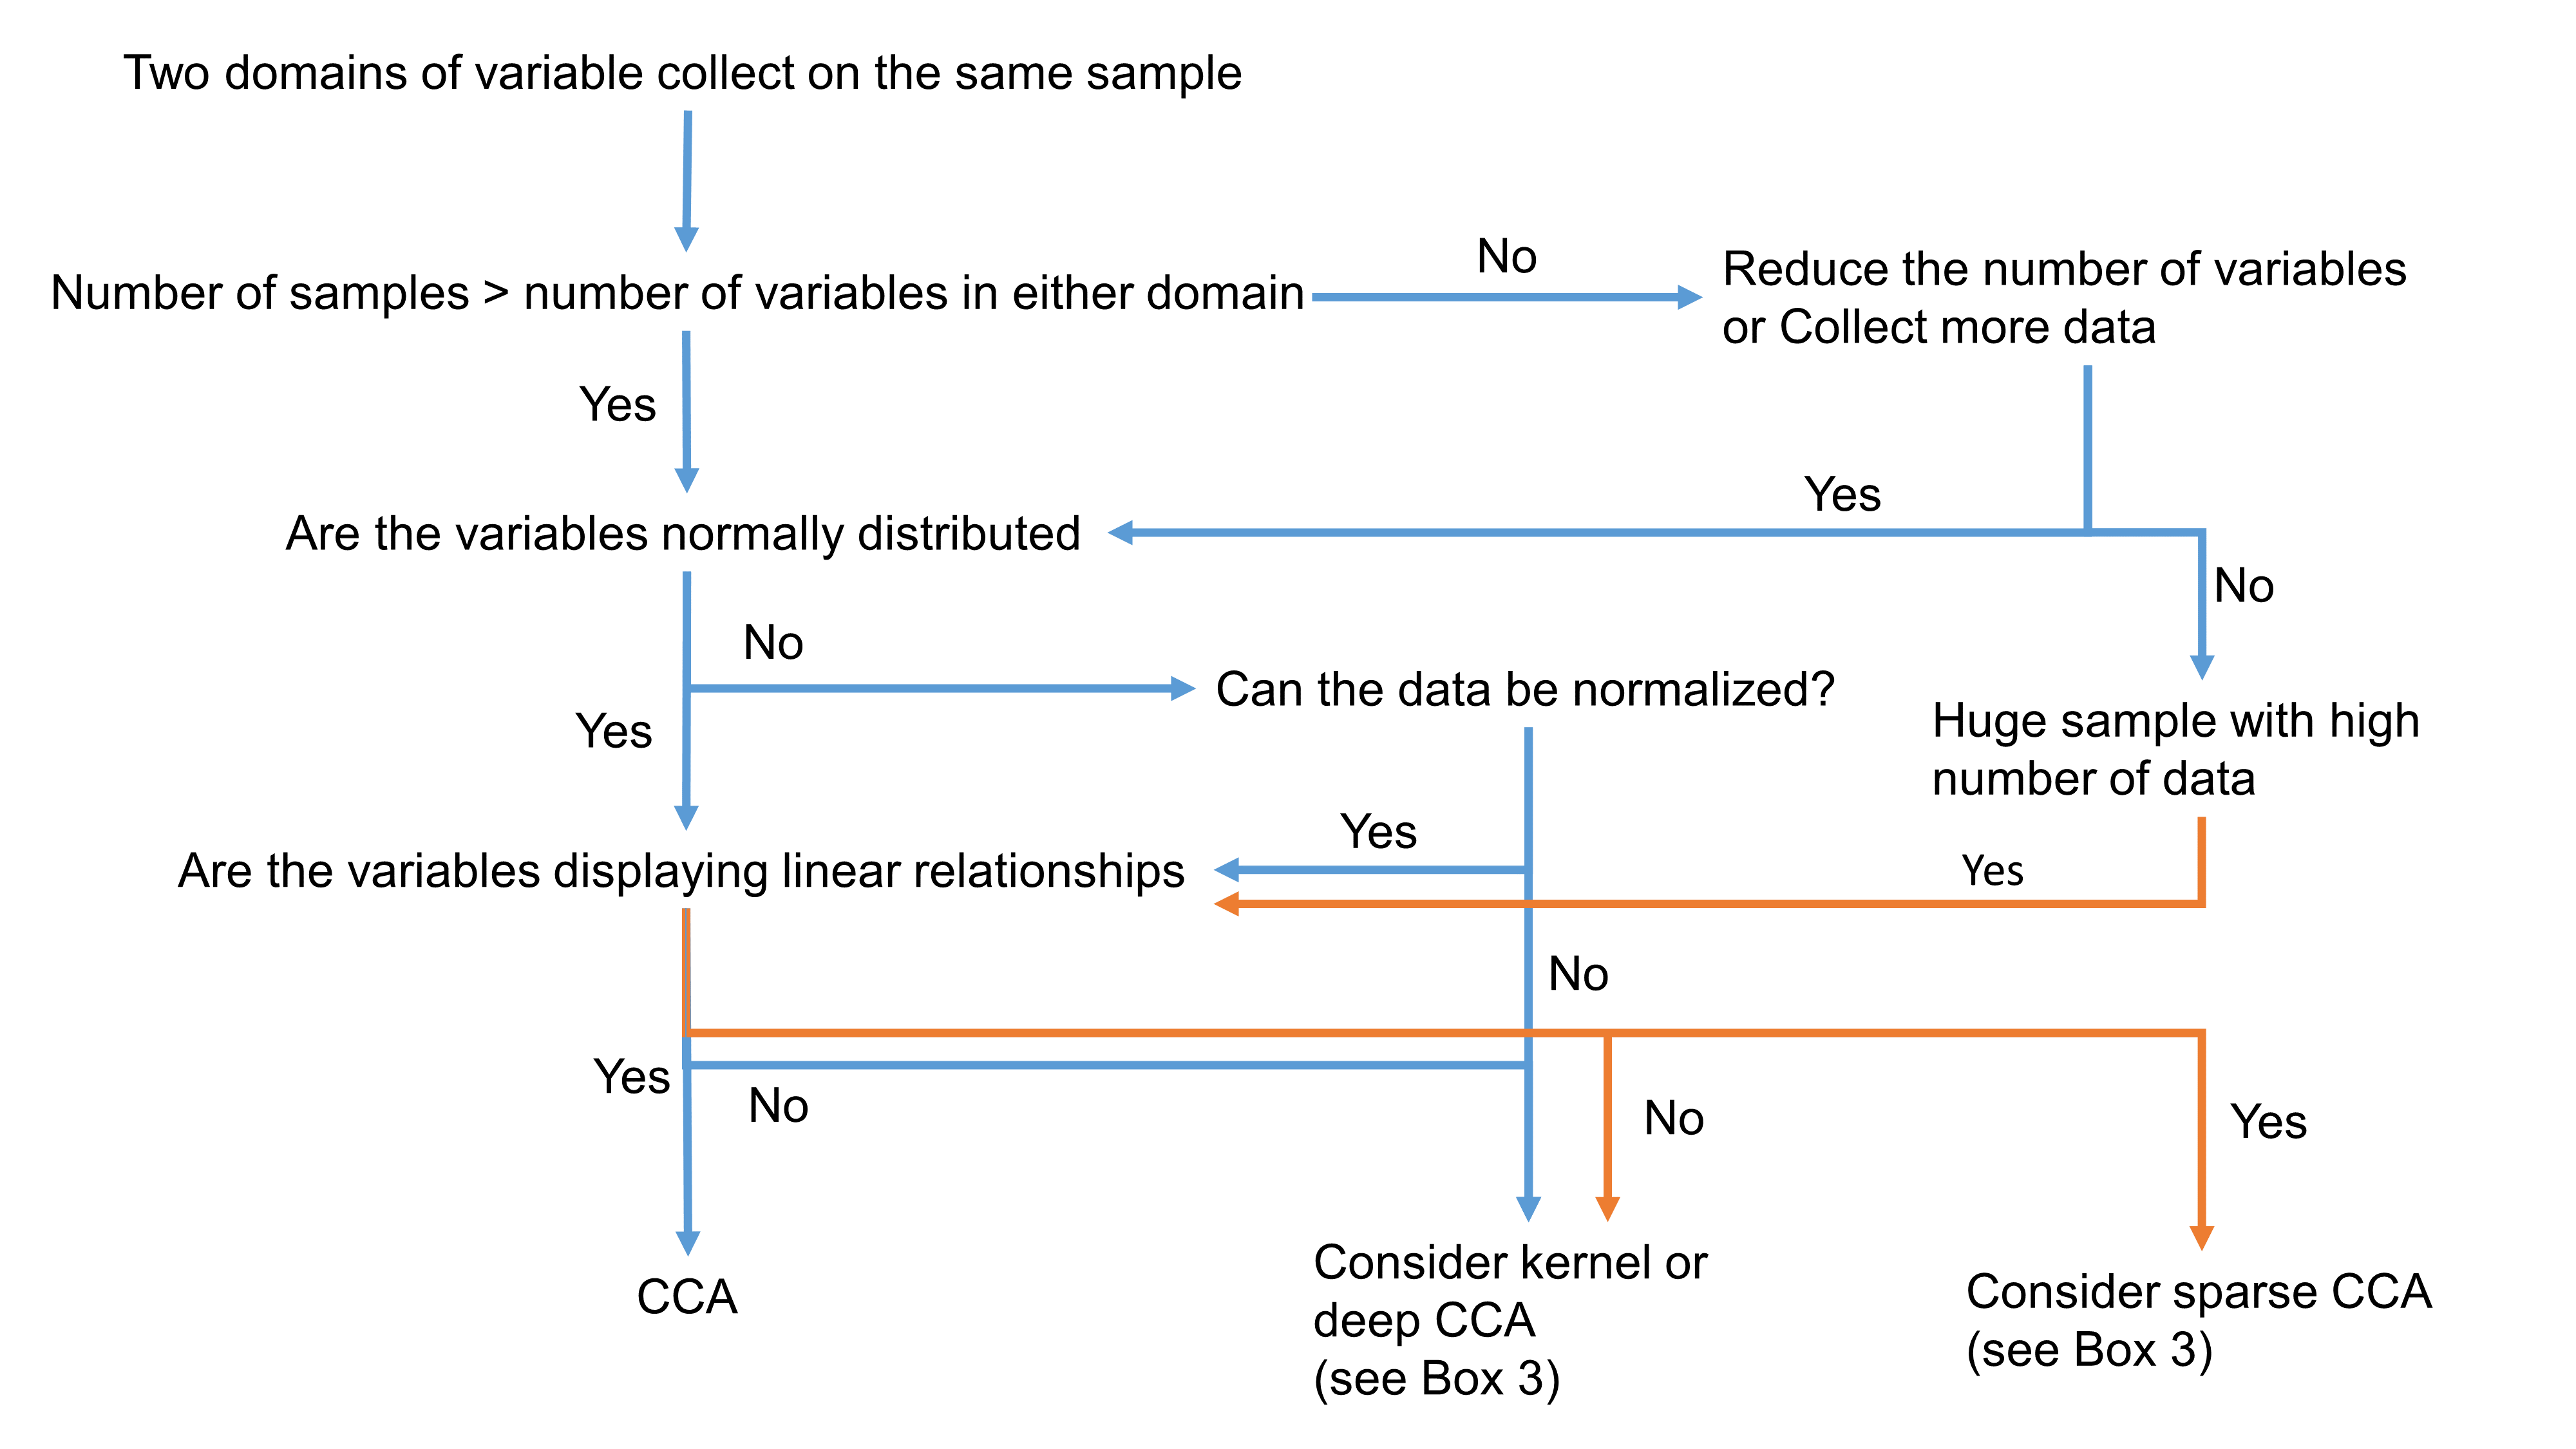
\includegraphics[width=1\textwidth]{cca/image/ccafig4.png}
	\caption{A flow chart illustrating the choices when considering the application of CCA to a data set.}
	\label{fig:methods:fig4}
\end{figure}

The structure of CCA is essentially a linear model, hence some limitations stem from the assumptions of normality and linearity. CCA can accommodate any metric variable without the strict assumption of normality. However, normality is desirable because it allows for the highest correlation among the variables. It is highly recommended to evaluate the normality of all variables and apply data transformation if possible. CCA uncover the linear relationships among the variables of interest. The linear assumption introduces two limitations to CCA. Firstly, since only linear effects can be captured, non-linear effects will not be captured. Data transformation or alternative CCA variation would be the solutions (see Relation to other commonly used methods). Secondly, the optimization objective is about correlation in CCA (i.e. see Interpretation). The discovered relationships are not necessarily accurate predictions in future data. Any interpretation and application related to predictability of the canonical components should be treated with caution. 
\newpage
\begin{infobox}{Overcoming the limitations of linear CCA}
Several useful extensions of CCA has emerged in the past decade to overcome the limitation of the linear version of CCA. The first was the nonlinear version of CCA, with \textbf{kernelization of CCA} (KCCA; Hardoon et al., 2004) as the representative.  Kernels are methods of implicitly mapping data into a higher-dimensional feature space with kernel function, a method known as the kernel trick. KCCA first project the data into a higher-dimensional feature space before performing CCA in the new feature space.  While KCCA allows learning of nonlinear representations, the drawback is that the representation is limited by the fixed kernel. KCCA is a nonparametric method, hence, the time required to train KCCA or compute the representations of new data points scales poorly with the size of the training set.

\textbf{Sparse CCA} (SCCA; Witten \& Tibshirani, 2009) is a method for identifying sparse linear combinations of the two sets of variables that are highly correlated with each other. It has been shown to be useful in the analysis of high-dimensional data, when the variable number of either arrays is higher than the number of samples. The sparse feature reduces the some coefficients to 0 in the linear structure depending on the penalty parameters. The benefit of sparsity is improvement in interpretation and feature selection. However, sparsity violates the orthogonality of CCA, meaning the components in different modes can correlate with each other. The explained variance of each mode will not follow the rank order either. Recently, we have used k-fold cross validation to identify the ideal level of sparsity in a study that explores the relationship between patterns of thought at rest and the associated brain organization (Wang, Bzdok et al., 2018).

With the recent advance in deep neural network, \textbf{deep CCA} (DCCA; Andrew et al., 2013) has been proposed as an alternative to KCCA as a non-linear method for CCA. Deep neural network is an algorithm that learns the representation of data through multiple non-linear transformations. The name came from the architecture that loosely follows the connections of neurons. DCCA simultaneously learns two deep neural network mappings of two variable sets that are maximally correlated. The main advantage is the faster performance over KCCA, because DCCA directly learns the data without re-mapping data into a higher dimension. 
\end{infobox}


% ==========================================================================================================


\section{Practical considerations}
\label{ch:methods:impliment}

Having introduce the features and interpretations of CCA, we would like to arise some practical considerations for the implementation. The computation of CCA is available in the in-built library of MATLAB (canocorr) and R (cancor), and Python machine-learning library scikit-learn (sklearn.cross\_decomposition.CCA). All implementations above provides comprehensive documentation of the basic usages. In the current section, we would like to mention details and problems that might happen while performing CCA on real data.

\subsection{Preprocessing}
Some minimum data preprocessing is required due to the linear nature of CCA. The objective of CCA is maximizing correlations. The nature of correlation is defined by the simultaneous unit change of the two variables; therefore, the computational process has implicitly standardize the data. The features obtained from CCA are therefore scale invariant.  (cf. PLS optimizes the covariance; therefore, the output will be influence by scaling.) Scaling, such as z-transformation, is still recommended before performing CCA for the ease of interpretation. This helps people to focus on unit chance rather than absolute values of data. Linear relationship is sensitive to outlier effects. To avoid outliers skewing the results, replacing outliers with mean or median is highly suggested. Aside from outliers, some confound variables can also introduce unwanted effects. Confound variable removal is recommended as a preprocessing step to reduce the risk of finding non-meaningful associations. To perform confound removal, we can fit a linear regression composed of the confound variables on each of the variables. The residual would be the variable without influences of the confounds.  

When the number of variable exceed the number of sample, PCA is recommended as a dimension reduction step before the analysis. An example is the work by Smith and colleague (2015). The downside of this method is that we cannot directly map the result to the original data. To interpret the CCA solutions in the original data, Smith and colleague (2015) correlate the canonical variates to the original data to recover the relevant variate captured by the CCA component pair. 

CCA component can be ambiguous for interpretation, especially when a PCA dimension reduction is applied. An alternative solution is a  CCA+ICA method (Miller et al., 2016; Sui et al., 2010) has been proposed to overcome the issue of projecting the PCA-compressed back to the original space. In the original CCA+ICA approach, the assumption is that CCA extracted components are an incomplete decomposition with multiple possible source (i.e. patients vs controls). CCA first finds the correlated variance of the two variable set. After CCA, the canonical components are concatenated into one array. ICA is then applied to the canonical components to recover the source of the variance. The ICA step can be done in the full feature space by projecting the CCA components to the PCA components (Miller et al., 2016). The CCA+ICA approach achieves both high estimation accuracy and to provide the correct connection between two variable sets. The ICA step is especially useful in detection of independent components that contribute to the common solution extracted from the two variable sets. 

\subsection{Model selection}
To select the number of mode (canonical component pair, see 3.3 Multiplicity), we can use explained variance to determine the final number of modes. The calculation can be done by predicting the canonical components with the original score with a linear regression. Another solution is to calculate the family-wise error rate through permutation tests.  The permutation is done on one of the variable sets, and then perform CCA on the permuted null sample. The first canonical correlation of the null sample is compared with all the CCA modes extracted from the real data. The p-value for each mode is calculated as number of null canonical correlation higher than the given mode from real sample, divided by  the number of permutation.
The variations of CCA might need an extra step for hyperparameters selection, such as kernel type and penalty in KCCA, penalty in SCCA, and layer number in DCCA. A permutation or cross-validation scheme is recommended for hyperparameters selection. The permutation test on hyperparameter selection is set up in the same way as model selection, but focusing on the first canonical correlation only (For example, see Appendix A in Witten \& Tibshirani, 2009). In terms of cross-validation, the objective function for model selection can be the out-of-sample explained variance or the variance loss between the training set and the testing set. 

% ==========================================================================================================
\section{Summary}
\label{ch:methods:summary}
CCA is a doubly multivariate pattern analysis on two variable sets. With no directionality implied on either variable set, CCA enables more flexibility on the research questions. As the interest in multitask data and rich cognitive phenotyping in large dataset grows, CCA fulfills the need of a method that considers all possible variables in one analysis. With its ability to reduce the data to meaningful and concise information, CCA is a promising method for scientists who are interested in exploration of multivariate patterns in large data sets.
\chapter{Exploring the heterogeneity of on-going thought}
\chaptermark{Heterogeneity of on-going thought}
\label{ch:study1}
\setcounter{equation}{0}
% ==========================================================================================================
\textit{The following chapter has been adapted from:} Wang, H.-T., Poerio, G. L., Murphy, C. E., Bzdok, D., Jefferies, E., \& Smallwood, J. (2018). Dimensions of Experience: Exploring the Heterogeneity of the Wandering Mind. \textit{Psychological Science}, \textit{29} (1), 56-–71. doi:\url{10.1177/0956797617728727}\footnote{
J. Smallwood, E. Jefferies, H.-T. Wang, and C. Murphy designed the study. H.-T. Wang, C. Murphy, and G. Poerio collected the data. The connection-strength and sparse canonical-correlation analysis pipeline was constructed by D. Bzdok and H.-T. Wang. Data were analyzed by H.-T. Wang, C. Murphy, and G. Poerio under the supervision of D. Bzdok, J. Smallwood, and E. Jefferies. H.-T. Wang and J. Smallwood drafted the manuscript. G. Poerio and D. Bzdok provided critical revisions. All the authors approved the final version of the manuscript prior to submission.
}
% ==========================================================================================================
\section{Abstract}
The tendency for the mind to wander to concerns other than the task at hand is a fundamental feature of human cognition, yet the consequences of variations in its experiential content for psychological functioning are not well understood. Here, we adopted multivariate pattern analysis to simultaneously decompose experience-sampling data and neural functional-connectivity data, which revealed dimensions that simultaneously describe individual variation in self-reported experience and default-mode-network connectivity. We identified dimensions corresponding to traits of positive-habitual thoughts and spontaneous task-unrelated thoughts. These dimensions were uniquely related to aspects of cognition, such as executive control and the ability to generate information in a creative fashion, and independently distinguished well-being measures. These data provide the most convincing evidence to date for an ontological view of the mind-wandering state as encompassing a broad range of different experiences and show that this heterogeneity underlies mind wandering's complex relationship to psychological functioning.
% ==========================================================================================================

\section{Introduction}
\label{study1:intro}

Although people's minds frequently wander from events in the here and now, or any task being performed, the functional consequences of this state remain poorly understood \cite{Mittner2016,SeliTiCS2016,SmallwoodFrontiers2013}.
Some studies link mind wandering to unhappiness
\cite{Killingsworth2010};
others suggest it facilitates recovery from negative emotional states
\cite{PoerioFrontiers2016,RubyPlos2013}.
Mind wandering is associated with poorer performance on tasks that place high demands on executive functions
\cite{McVay2009,MrazekJoEP2012},
yet studies of problem solving suggest that mind wandering may promote creativity
\cite{Baird2012,Smeekens2016}.
This wide range of associated functional outcomes is puzzling--—if mind wandering is a homogeneous construct, then it is unclear why it should be associated with such a complex array of often opposing outcomes. To reconcile this contradictory evidence, researchers have suggested that mind wandering may be heterogeneous, encompassing multiple states with differential contents and underlying cognitive architectures \cite{SmallwoodFrontiers2013}. According to this ontological perspective, different functional associations arise from different `types' of experience, which explains the range of functional outcomes observed in the literature.

In the current study, we recruited 165 participants and obtained data on (a) the organization of the brain at rest using functional MRI (fMRI), (b) the content and form of experience recorded across different days, (c) cognitive functions assessed by a comprehensive battery of tasks (including memory, creativity, and executive control), and (d) psychological well-being via questionnaires. Our procedure is presented in \cref{fig:study1:fig1}. These data allowed us to use novel multivariate analysis methods to test the hypothesis that there are different types of mind wandering, with unique neural and experiential patterns accounting for unique variance in the psychological profile of our sample.

\begin{sidewaysfigure}[p]
	\centering
	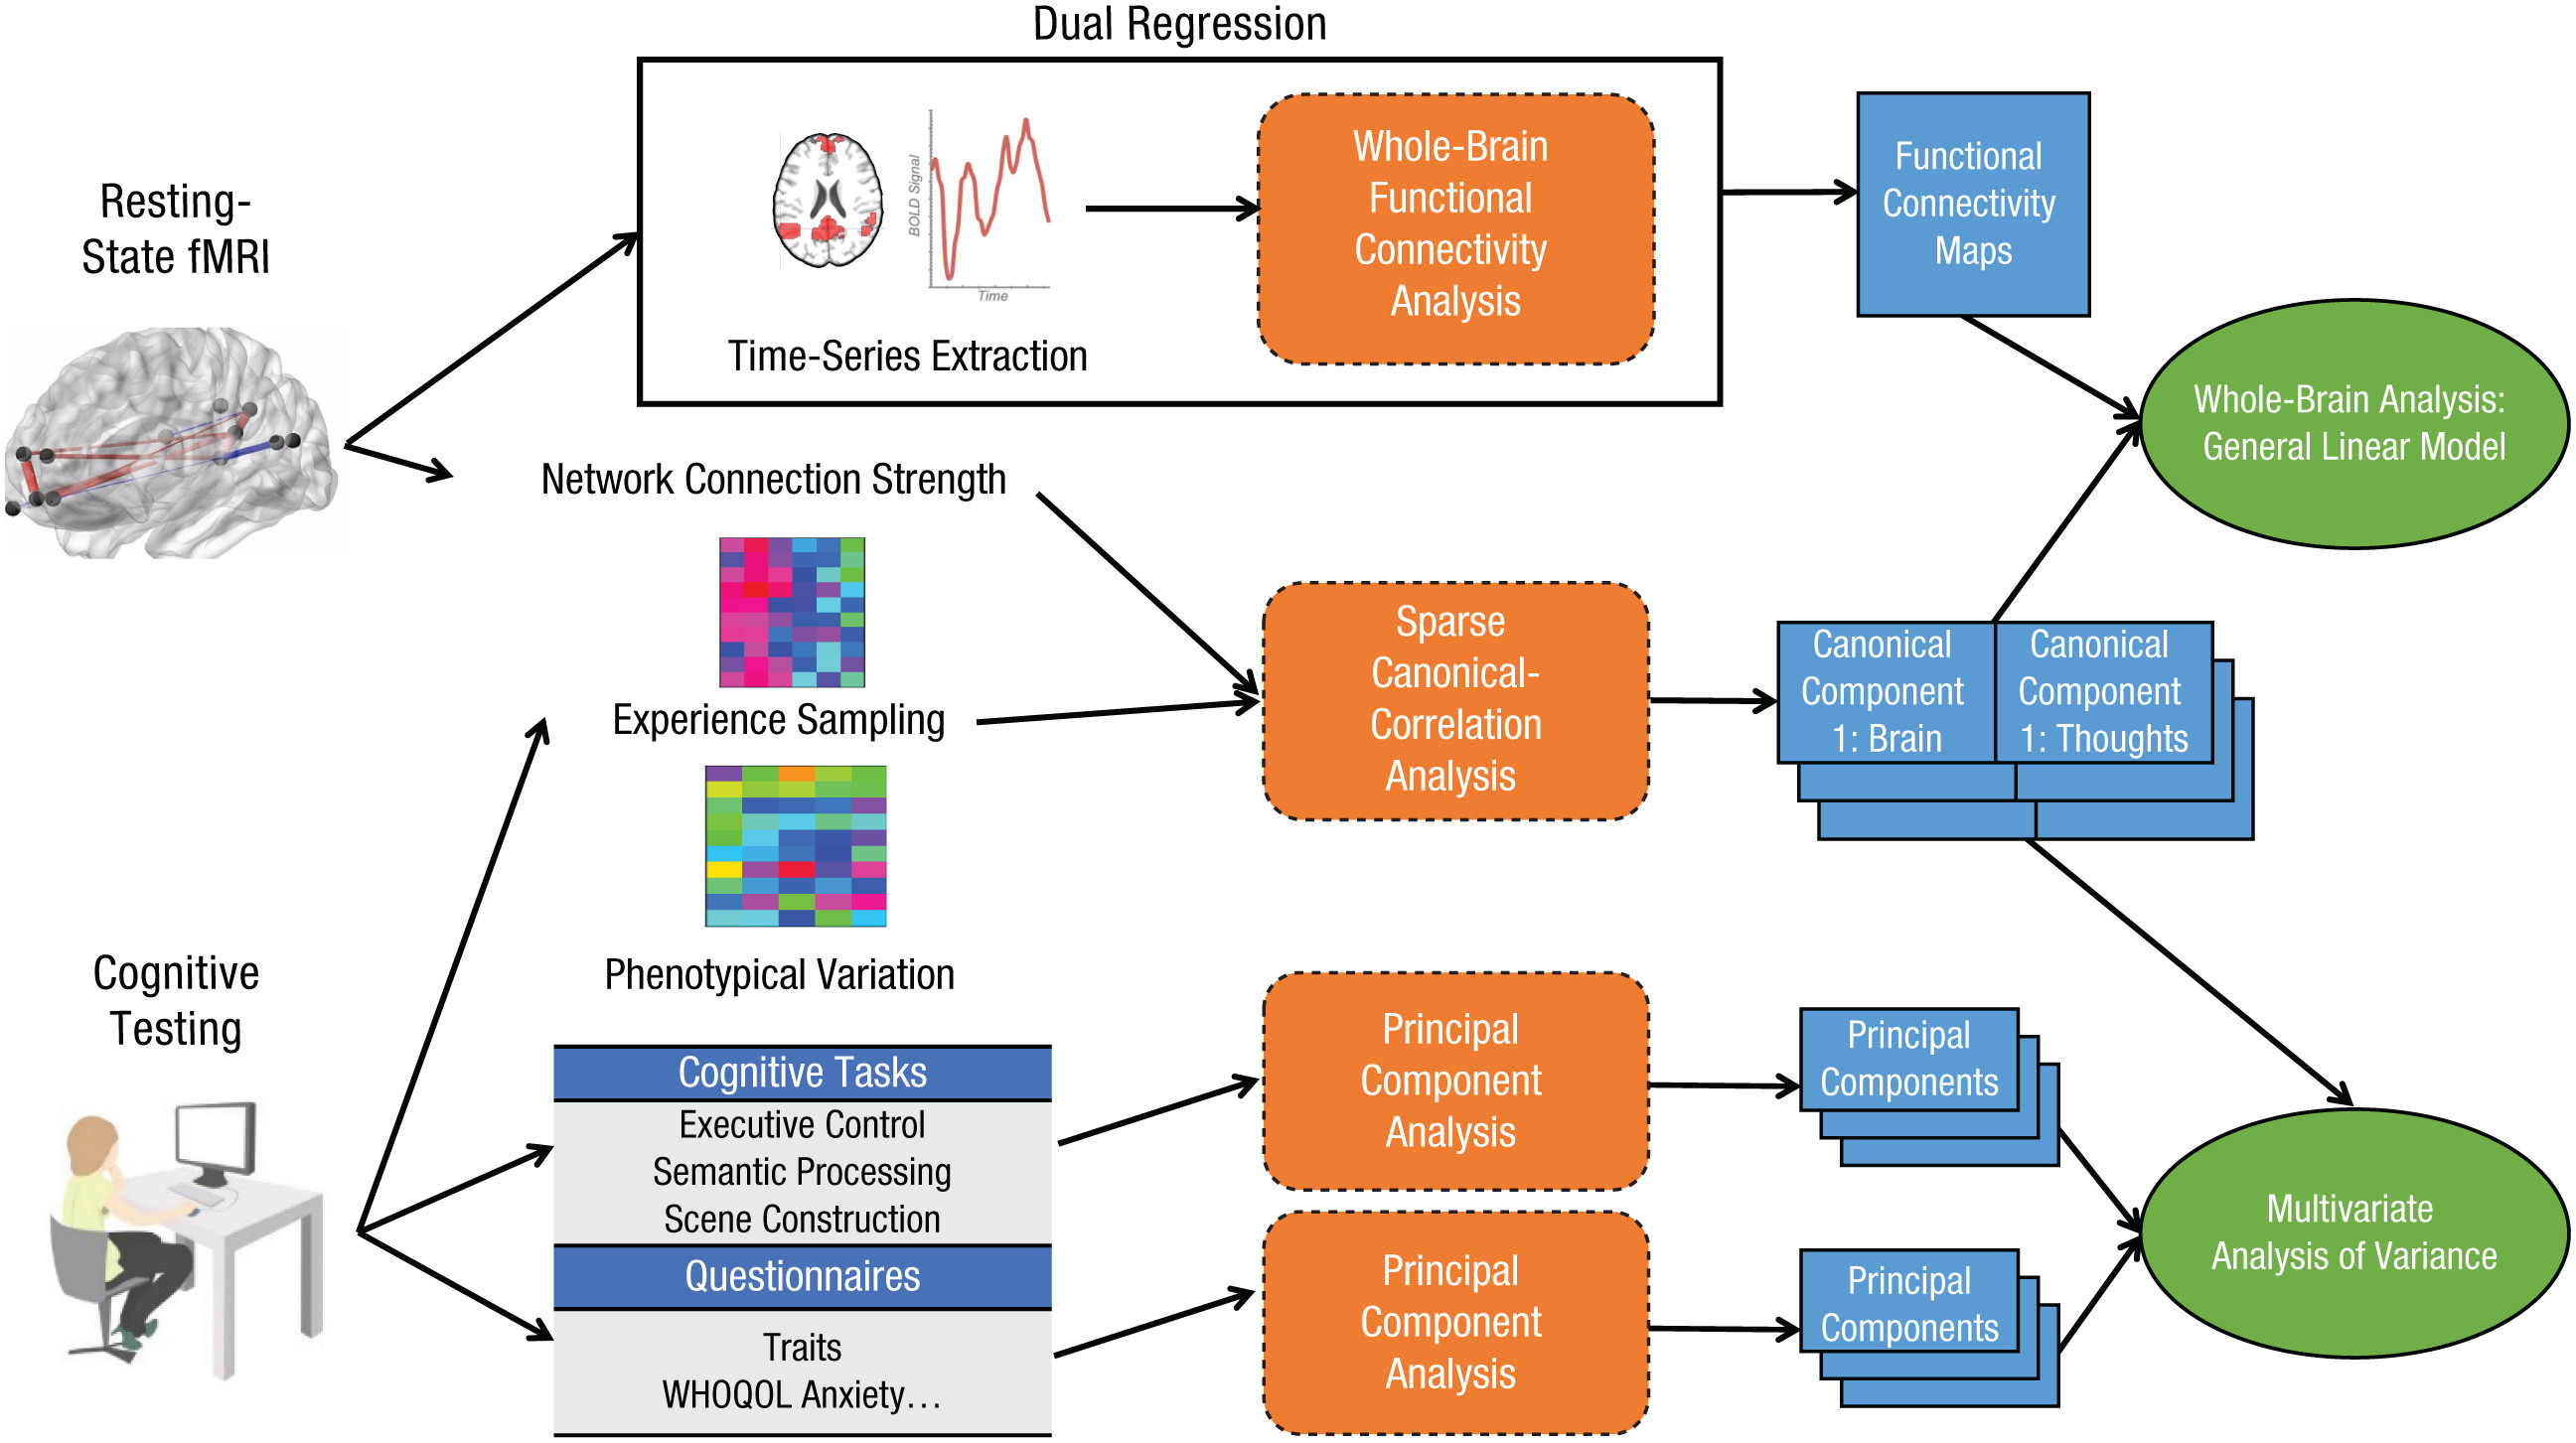
\includegraphics[width=0.8\textwidth]{study1/image/study1fig1.jpeg}
		\caption{Schematic of the procedure and analysis strategy employed in the current study.}
		\caption*{\footnotesize{We collected resting-state functional MRI (fMRI) data, cognitive-function measures, and questionnaires on personal traits for each participant. These were submitted to analysis (rectangles with dashed borders), which created latent components or features (rectangles with solid borders) for each subject, and these variables were subsequently passed to the main analysis (ovals). WHOQOL = World Health Organization Quality of Life assessment \cite{WHOQOL2002}.}}

	\label{fig:study1:fig1}
\end{sidewaysfigure}

We used functional connection strength to characterize the neural organization of each individual. We selected regions for our analysis on the basis of evidence that task-unrelated thoughts are linked to concurrent increases in activity in medial prefrontal cortex (mPFC), posterior cingulate cortex (pCC), and lateral parietal cortex
\cite<for meta-analyses, see>{Fox2015,Stawarczyk2015}.
—regions that make up the core of the default mode network
\cite<DMN;>{Buckner2008}.
During mind wandering, it is believed that these regions interact with other areas of the cortex, in particular, temporal lobe regions associated with memory representation that are also allied to the DMN. For example, the hippocampus activates early during mind wandering
\cite{Ellamil2016}.
whereas connectivity between lateral and medial aspects of the temporal lobe and the DMN core predicts individual variation in features of mind wandering, such as its episodic content
\cite{Karapanagiotidis2017}.
Contemporary accounts of mind wandering posit that the DMN may be important for automatic aspects of cognition
\cite{Christoff2016}.
Other studies have highlighted links with the lateral prefrontal cortex, which is important for executive control when mind wandering is more deliberate \cite<e.g.,>{Golchert2017}.

We applied multivariate pattern analysis to the neurocognitive and experiential data to identify different types of mind wandering. If the DMN is important for automatic aspects of cognition \cite{Christoff2016}, states linked to high levels of connectivity within this system may have experiential features reflecting more automatic types of cognition. Our a priori decision to focus on the DMN core to derive patterns of experience limited our ability to observe interactions with regions outside of this system, so we used whole-brain functional connectivity to characterize these links for each type of experience. On the basis of prior studies \cite<e.g.,>{Ellamil2016,Golchert2017,Smallwood2016}, we expected this analysis to identify connections with regions in the temporal lobe or the executive system. This pattern would confirm the hypothesised accounts of the DMN as important in integrating neural information \cite{Margulies2016,Smallwood2016}. Having characterised different types of mind wandering in both brain and experience, we used these to test the hypothesis that different categories of experience are related to different functional outcomes. We performed an individual differences analysis to understand whether our characterised types of mind wandering have unique functional associations, including better creativity, worse executive control, and lower levels of well-being. We expected different patterns of experience to capture different psychological profiles explaining the heterogeneous pattern of functional outcomes that have been linked to the mind-wandering state in previous studies
\cite{SmallwoodCC2013}.

% ==========================================================================================================

\section{Method}
\label{study1:method}
\subsection{Participants}
\label{study1:method:a}

One hundred sixty-five healthy participants were recruited from the University of York (99 females, 66 males; age range = 18--31 years, \textit{M} = 20.43, \textit{SD} = 2.63). We preselected a sample size approximately double those used in our prior studies \cite<e.g.>{Smallwood2016}.%(e.g., Smallwood et al., 2016).
A sample size of at least 125 is recommended in order to have 95\% confidence that a correlation of typical size (\textit{r} = .20--.30) is present and greater than 0
\cite{Hemphill2003}.
Participants were right-handed native English speakers with normal or corrected-to-normal vision and no history of psychiatric or neurological illness. Participants underwent MRI scanning, completed an online questionnaire, and then attended three 2-hr behavioural testing sessions to complete a battery of cognitive tasks. The behavioural sessions took place within a week of the scan. Eight participants were excluded from the multivariate pattern analysis because they failed to complete all of the behavioural testing sessions. In total, 157 participants were included in the multivariate pattern analysis and the comparison with cognitive performance. One hundred forty-two participants completed both the behavioural testing sessions and questionnaires and were included in the analysis associated with well-being. Participants were rewarded with either a payment of \pounds 80 or a commensurate amount of course credit. All participants provided written consent prior to the fMRI session and the first behavioural testing session. Approval for the study was obtained from the ethics committee of the University of York Department of Psychology and the University of York Neuroimaging Centre.

\subsection{MRI acquisition}
\label{study1:method:b}
Structural and functional data were acquired using a 3T HDx Excite MRI scanner (GE Healthcare, Little Chalfont, United Kingdom) utilising an eight-channel phased-array head coil tuned to 127.4 MHz at the York Neuroimaging Centre, University of York. Structural MRI acquisition in all participants was based on a T1-weighted 3-D fast-spoiled gradient-echo sequence— repetition time (TR) = 7.8 s,
echo time (TE) = minimum full,
flip angle = \ang{20},
matrix size = 256 $\times$ 256, 176 slices,
voxel size = \SI[product-units=power]{1.13 x 1.13 x 1}{\mm}.
Resting-state activity was recorded from the whole brain using single-shot 2-D gradient-echo-planar imaging—TR = 3 s, TE = minimum full,
flip angle = \ang{90},
matrix size = 64 $\times$ 64, 60 slices,
voxel size = \SI[product-units=power]{3 x 3 x 3}{\mm}, 180 volumes.
Participants viewed a fixation cross for the duration of the 9-min fMRI resting-state scan. A fluid-attenuated inversion-recovery (FLAIR) scan with the same orientation as the functional scans was collected to improve co-registration between subject-specific structural and functional scans.


\subsection{Questionnaires}
\label{study1:method:c}

We administered a battery of questionnaires to comprehensively assess a diverse range of trait-level individual differences that have been previously related to mind wandering. These questionnaires captured the trait-like features of participants’ psychological states, particularly aspects of well-being. The complete details of the questionnaires are presented in \cref{appendix:study1:subsection1}.

\subsection{Behavioural testing sessions}
\label{study1:method:d}
The trait profiles captured by the questionnaires were complemented by measures of performance on a range of cognitive tasks. Behavioural tasks were selected to measure a broad range of cognitive attributes, including semantic and episodic memory, executive control, fluency, and creativity. These measures were assessed in three sessions. Each session began with a task to index the content and form of mind wandering (0-back/ 1-back task), followed by the other cognitive measures. The order of sessions and the order of tasks was counterbalanced across individuals. Details of the 0-back/ 1-back task are presented in the following paragraph. The complete details of the other cognitive tasks are described in \cref{appendix:study1:subsection2}.

Using a block design, we assessed the contents of experience during mind wandering in the context of a simple task that manipulated working memory load
\cite<see>[for prior published examples of this task]{Konishi2015,Medea2016}.
This task was performed at the beginning of each laboratory session to minimise participant fatigue. Measuring experience over 3 days provided us with a more comprehensive description of participants’ trait-level mind wandering than would have been possible in a single experimental session.

In both tasks, participants completed target and nontarget trials. In nontarget trials, a pair of shapes appeared on screen; the two shapes were separated by a vertical line. The pairs consisted of a circle and a square, a circle and a triangle, and a square and a triangle, each in two different left/right configurations for a total of six possible pairs. Following an unpredictable sequence of nontarget trials, a target trial was presented in which participants had to make a manual response. The target was a small stimulus presented in either blue or red across conditions, with the colour counterbalanced across participants. In the 0-back condition, the target was flanked by one of two shapes, and participants had to indicate which shape matched the target shape by pressing the appropriate button. In the 1-back condition, the target was flanked by two question marks, and participants had to respond depending on which side the target shape had been on during the prior trial. Responses were made using the left and right arrow keys. Presentation times for fixation crosses ranged from 1.3 to 1.7 s in steps of 0.05 s, and nontarget presentation times varied from 0.8 to 1.2 s in steps of 0.05 s. Target presentation times always ranged from 2.1 to 2.5 s in steps of 0.05 s, and a response from participants did not end the target presentation.

There were eight blocks in one session, and each block consisted of two to four miniblocks. Each block contained either the 0-back or 1-back condition. The change of task was signalled by the presentation of the word “SWITCH,” which remained on screen for 5 s. The order of the tasks was counterbalanced across participants, and the eight blocks lasted around 25 min. In each mini-block, there was one target trial, and the number of nontarget trials preceding the targets varied between one and six. Participants’ performance was measured by their efficiency, which was calculated by dividing their average response time by their accuracy. For ease of interpretation, efficiency scores were reversed, so that higher scores indicated better performance.

In order to sample different features of participants’ ongoing experiences, we used multidimensional experience sampling
\cite<MDES;>{Medea2016,RubyPlos2013,Smallwood2016}.
This technique uses self-report data to assess the contents of experience on a number of dimensions. The first thought probe asked participants to rate their level of task focus (“My thoughts were focused on the task I was performing”) on a sliding scale from 0 (\textit{completely off task}) to 1 (\textit{completely on task}). Participants then answered 12 randomly presented questions regarding the content and form of their experience at the moment just before they answered the first thought probe (on level of task focus). These questions (described in \cref{tab:study1:1}) were based on those used in prior studies adopting this approach to measure self-generated thought
\cite{Medea2016,RubyPlos2013,Smallwood2016}.
At the moment of target presentation, there was a 20\% chance of a thought probe being presented instead of a target, with a maximum of one probe per block of the 0-back/1-back task. In each session, an average of 14.07 (\textit{SD} = 3.30, range = 6--25) MDES probes occurred; in the 0-back condition, an average of 7.02 (\textit{SD} = 2.36, range = 2--14) MDES probes occurred; and in the 1-back condition, an average of 7.04 (\textit{SD} = 2.24, range = 1--15) occurred. In total, we sampled 7,006 examples of experience in this study. We calculated the mean scores of each question across the three sessions for each participant. The MDES scores were first transformed into z scores for mean-centring and univariance scaling. The scores described the average momentary experience in each dimension. We used this score in the multivariate analysis later.

\linespacesmall
\begin{table}
\centering
\caption{Experience-Sampling Questions in the 0-Back/1-Back Task.}
\label{tab:study1:1}
\resizebox{\textwidth}{!}{
\begin{tabular}{ l l c c}
\toprule
& & \multicolumn{2}{c}{Response scale} \\ \cmidrule{3-4}
Dimension & \multicolumn{1}{c}{Question} & 0 & 1 \\ \midrule
Focus & My thoughts were focused on the task I was performing.  & \textit{Not at all} & \textit{Completely} \\
Future & My thoughts involved future events. & \textit{Not at all} & \textit{Completely} \\
Past & My thoughts involved past events. & \textit{Not at all} & \textit{Completely} \\
Self & My thoughts involved myself. & \textit{Not at all} & \textit{Completely} \\
Other & My thoughts involved other people. & \textit{Not at all} & \textit{Completely} \\
Emotion & The content of my thoughts was: & \textit{Negative} & \textit{Positive} \\
Images & My thoughts were in the form of images. & \textit{Not at all} & \textit{Completely} \\
Words & My thoughts were in the form of words. & \textit{Not at all} & \textit{Completely} \\
Vividness & My thoughts were vivid as if I was there. & \textit{Not at all} & \textit{Completely} \\
Detail & My thoughts were detailed and specific. & \textit{Not at all} & \textit{Completely} \\
Habit & This thought has recurrent themes similar to those I have had before. & \textit{Not at all} & \textit{Completely} \\
Evolving & My thoughts tended to evolve in a series of steps. & \textit{Not at all} & \textit{Completely} \\
Deliberation & My thoughts were: & \textit{Spontaneous} & \textit{Deliberate} \\ \bottomrule
\end{tabular}
}
\end{table}
\linespacenormal

\subsection{Neuroimaging data preprocessing and analysis}
\label{study1:method:e}

\subsubsection{Resting-state fMRI.}

Functional and structural data were preprocessed and analysed using the Oxford Centre for Functional MRI of the Brain’s (FMRIB’s) Software Library (FSL Version 4.1, \url{http://www.fmrib.ox.ac.uk/fsl}).
Individual FLAIR and T1-weighted structural brain images were extracted using FSL’s Brain Extraction Tool (BET). Structural images were linearly registered to the MNI152 template using FMRIB’s Linear Image Registration Tool (FLIRT). The resting-state functional data were preprocessed and analysed using FSL's FMRI Expert Analysis Tool (FEAT). The individual-subject analysis involved motion correction using FSL’s MCFLIRT, slice-timing correction using Fourierspace time-series phase shifting, high-pass temporal filtering (Gaussian-weighted least-squares straight-line fitting, \(\sigma\)= 200 s), and Gaussian low-pass temporal filtering (\(\sigma\) = 2.8 s). In addition, we regressed out six motion parameters (as estimated by MCFLIRT) and regressing out cerebrospinal fluid and white-matter signal (top five components in the principal component analysis, PCA; CompCor method). No spatial smoothing and no global signal regression were applied.

\subsubsection{Network-strength analysis.}

To describe the functional architecture of the DMN, we transformed the resting-state blood-oxygen-level-dependent time series into connection strength values of the selected regions for each participant. The regions of interest (ROIs) were obtained from connectivity-based functional parcellation studies of the DMN by Bzdok and colleagues
\cite{BzdokNI2013,Bzdok2015,Bzdok2016,Eickhoff2016,Eickhoff2016}.
There were 16 selected target network nodes, including subregions located in the bilateral temporoparietal junction (TPJ), ventromedial prefrontal cortex (vmPFC), dorsomedial prefrontal cortex (dmPFC), and posteromedial cortex
(PMC; see \cref{fig:study1:fig2}a).
The ROI masks and the related functional-connectivity network produced with Neurosynth core tools
(\url{http://github.com/neurosynth/neuro_synth})
can be found on NeuroVault
(\url{http://neurovault.org/collections/2275/}). First, we extracted and then averaged the time series of all voxels within the 6-mm sphere masks of the given regions. Second, we created \(16\times16\) symmetrical correlation matrices representing the network of the regions that was computed for all the individual subjects. The off-diagonal of each correlation matrix contained 120 unique region-region connection strengths. This approach provided a measure of connection strength of the region-region coupling of the DMN for each participant.

\begin{sidewaysfigure}[p]
	\centering
	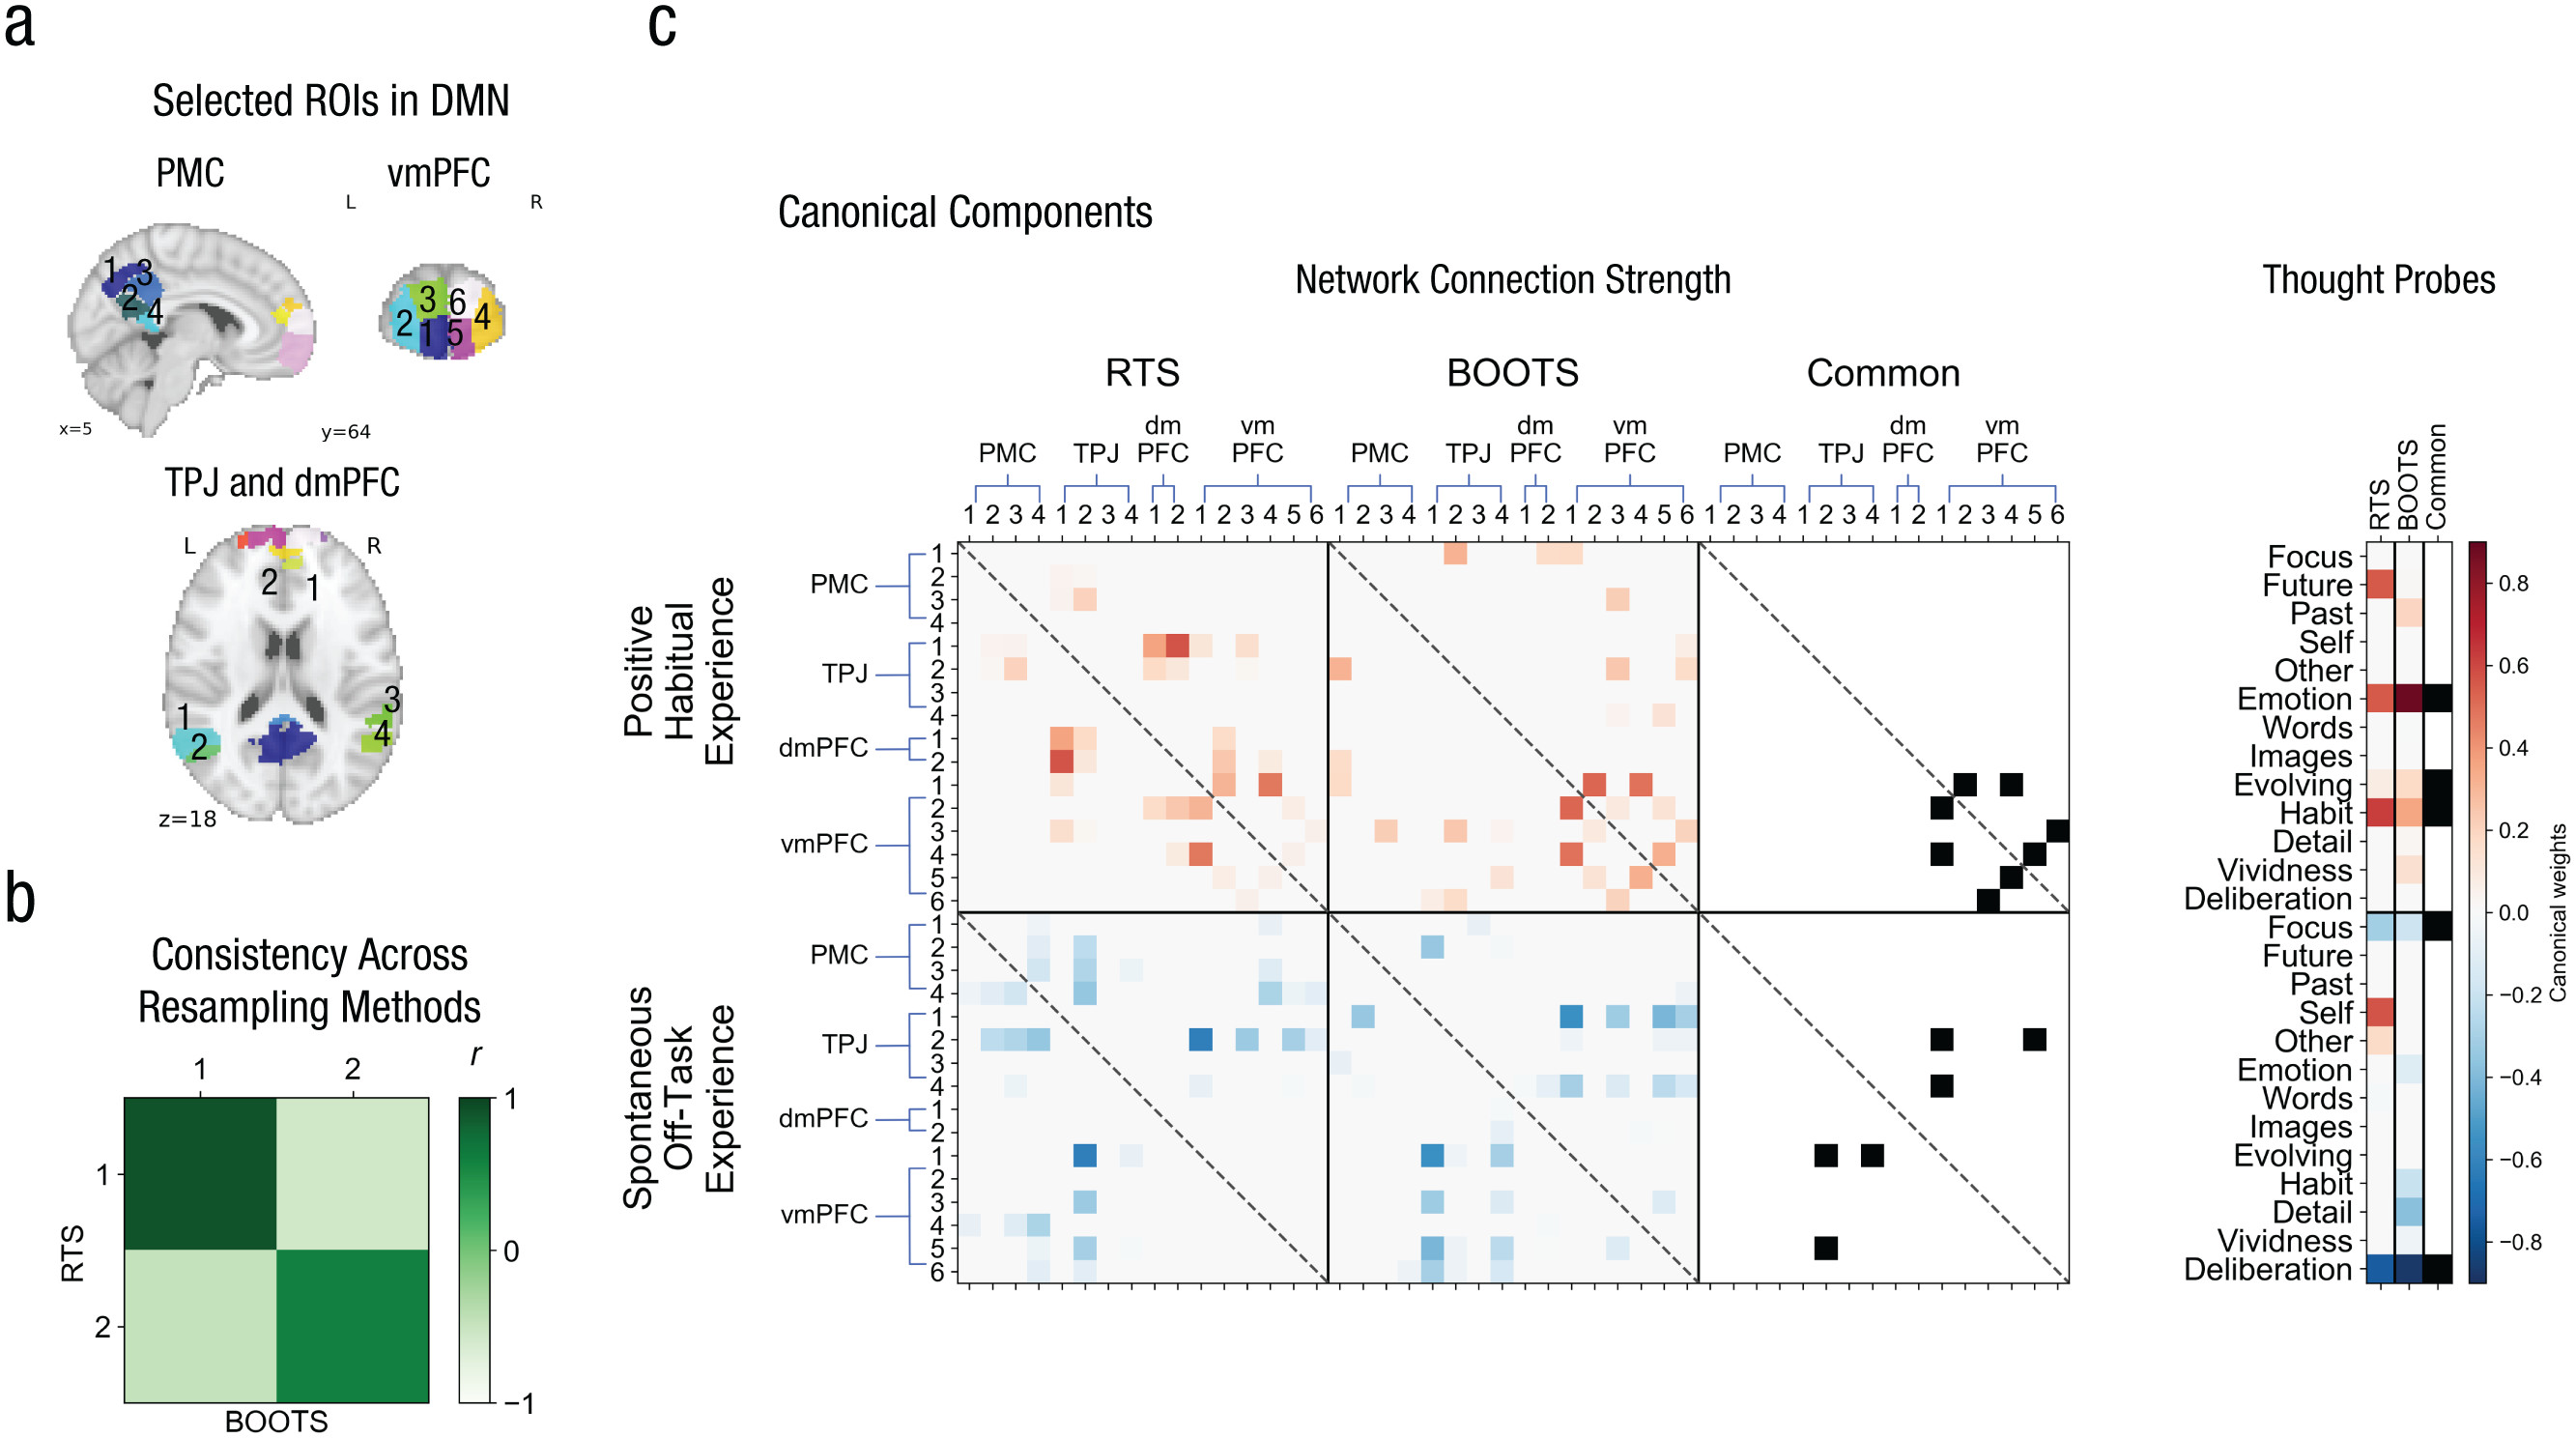
\includegraphics[width=0.8\textwidth]{study1/image/study1fig2.jpeg}
	\caption{Results of the sparse canonical-correlation analysis.}
	\caption*{\footnotesize{The regions of interest (ROIs) of the default mode network (DMN) from which the network connection strength was calculated are shown in (a). The correlation between the two canonical components (positive-habitual experience, 1, and spontaneous off-task experience, 2) and the two analyses is shown in (b). The analyses were restricted temporal sampling (RTS), which describes the canonical components produced when the data from 1 day of each participant were randomly removed from the decomposition, and bootstrapping (BOOTS), which describes the solution produced using bootstrapping. Panel (c) shows the results of the sparse canonical-correlation analysis (SCCA) conducted on the network-connection-strength values of key nodes of the DMN at rest and self-reports of experience during a laboratory task. Results are shown separately for the two components of experience for each analysis. Also shown are the common findings between the two analyses. The numbers indicate the subregions of each ROI, as indicated in (a). For the questions associated with each self-report dimension, see Table 1.}}

	\label{fig:study1:fig2}
\end{sidewaysfigure}

\subsubsection{Multivariate pattern analysis.}

We performed a sparse canonical-correlation analysis (SCCA) on the connection strength data and MDES scores to yield different dimensions that simultaneously described neural organisation and experience. Canonical correlation analysis (CCA) is an advanced multivariate technique that identifies distinct components between two variables spaces \cite{Hardoon2004}--in our case, brain-region connection-strength values and experiential reports obtained through MDES. This modelling approach allows linear combinations of the two variable vectors with correlations among variables to be determined and, unlike in PCA and independent component analysis, produces dimensions in which the biological data are simultaneously constrained by psychological measures (and vice versa). To enhance the interpretability of the decomposition solutions, we used a variant of CCA penalised by L\textsubscript{1} regularisation, SCCA \cite<see>{Hastie2015}. This was achieved by setting a maximum number of brain or behaviour variables to exactly zero, which resulted in a regularised version of the singular value decomposition. A reliable and robust implementation of the SCCA method was retrieved as an R package from CRAN (penalized multivariate analysis, or PMA). In the current analysis, the L\textsubscript{1} penalty was set to 0.3 on resting-state functional connectivity and to 0.5 for the MDES results. Other parameters were set to the default. In this way, our analysis performed low-rank (i.e., described an overall network pattern by a parsimonious set of connectivity causes), conjoint (i.e., respected variance in brain and behaviour at once), and sparse (i.e., automatically found unimportant variables) decomposition of experiential and neural data.

\subsubsection{Stability analyses.}

We performed two analyses to assess the stability of the solutions produced by SCCA. First, for each participant, we excluded the MDES data of 1 random day and then recalculated the average scores for these questions. We repeated the decomposition on this new set of MDES data and the network connection strength. This corroborative quantitative assessment provided insight into the robustness of the obtained findings by a permutation analysis that left 1 day out at a time. In particular, this procedure addressed whether either the first day (when participants may be learning how to respond to the experience-sampling method) or the last day (when participants may have lower levels of motivation) might unduly bias the decomposition solutions. We reasoned that if the average momentary MDES responses are stable across three sessions, then they should yield similar latent components. Second, we acquired bootstrap samples as a permutation analysis to estimate the variance and generalisability of the sample to the population. The bootstrap resamples, each reflecting an alternative data sample that we could have obtained from the same distribution, was created by random sampling with replacement. The identical SCCA computation was then reiterated individually on each of the 1,000 perturbed versions of the actual data sample. This approach enables quantitative assessment of the quality of the original SCCA estimates by inferring confidence intervals (see \cref{fig:3S1} in \cref{appendix:study1:subsection3} for the distributions). We selected latent components that were consistent across the decomposition of the original sample, a leave-1-day-out sample, and a bootstrap sample, as those are the stable components that were less biased by the session effect and closer to our best estimation of population. We formalised the similarity of these two types of resampling by conducting a formal conjunction of the solutions generated through these different methods of resampling. To quantify the similarity between the components, we performed a conjunction that highlights the common elements of each solution. The feature conjunctions were calculated as follows:

\begin{equation}
  \text{conjunction}=
  \begin{cases}
    1, & \text{when}
    \sqrt{
    \text{weight\textsubscript{LODO}}
    \times
    \text{weight\textsubscript{BOOTS}}
    } < 0.1\\
    0, & \text{otherwise}.
  \end{cases}
\end{equation}

where LODO refers to leave 1 day out and BOOTS refers to bootstrapping. In addition, because bootstrapping produces a population estimation of our sample, we used the latent component weights produced by this method to compute component scores. This set of scores was used in all subsequent analyses. The source code for this analysis is available at \url{https://github.com/ htwangtw/DimensionsOfExperience}.

\subsubsection{Whole-brain analysis.}

A limitation in our analysis is that we focused on the DMN to describe patterns of thought. To overcome this limitation, we generalised the types of experience provided by the SCCA by assessing their associations with areas outside of the DMN using a process conceptually similar to dual regression \cite{DualRegression2009}. To perform these analyses, we preprocessed and analysed the resting-state functional data using FEAT. For the individual-subject preprocessing procedure, see the Resting-State fMRI section.

Following these preprocessing steps, we used a mask produced by the average of the DMN ROIs to determine the time series that described this neural system. This time series was used in a whole-brain functionality analysis for each participant. This allowed us to produce a subject-specific spatial map based on the selected ROIs, and these maps were used as dependent measures in our group-level analysis. To test whether the functional connectivity of the DMN ROIs was associated with the canonical components, we conducted a group-level analysis using FMRIB’s Local Analysis of Mixed Effects Stage 1 (FLAME 1). To control for spurious correlations that might emerge from movement, we included the two canonical components on thought reports only, group mean and Jenkinson’s mean framewise displacement \cite<FD>{Jenkinson2002}, as explanatory variables in the full model. The Jenkinson’s mean FD was calculated by the motion power statistic function in Configurable Pipeline for the Analysis of Connectomes
(C-PAC; \url{https://fcp-indi .github.io/}).
A 50\% probabilistic gray-matter mask was applied to the results maps, and the results were thresholded at the whole-brain level using cluster-based Gaussian random-field theory, with a cluster-forming threshold (\(\mathit{Z}\)) of 2.6 and a familywise-error-corrected cluster significance level (\(\mathit{p}\)) of .05. Unthresholded maps were uploaded onto Neurovault
(\url{http://neurovault.org/images/43189/}).

\subsubsection{PCA.}
To summarise the questionnaire and task data, we performed an initial data-reduction step using PCA in SPSS (Version 24). This analysis was performed separately for the questionnaires and task measures. One hundred forty-five participants’ data were included in the analysis of the questionnaire items, and 157 participants’ data were included in the analysis of the behavioural tasks. The behavioural-task measures were converted into \(\mathit{z}\) scores to avoid data distortions derived from the difference in score means. Missing data were imputed by mean scores in both analyses. The Kaiser-Meyer-Olkin (KMO) measure and Bartlett’s test of sphericity were used to measure the sampling adequacy of the model. Components were selected on the basis of the elbow in a scree plot (see \cref{fig:3S2} in \cref{appendix:study1:subsection3}), and varimax rotation was used to maximise the distinctiveness of each solution.

In the PCA of the phenotypical variation measured by behavioural tasks, Bartlett’s test of sphericity was significant,
\(\chi^{2}(210) = 775.01\),
\(\mathit{p} < .001\),
which indicates that it is appropriate to apply PCA to these data. The KMO measure of sampling adequacy indicated that the current sample was acceptable for PCA (KMO = 0.79). The PCA of task performance revealed three principal components with a clear elbow after the third component observed in the scree plot. The three orthogonal components accounted for 40.7\% of the total variance; the component loading patterns are shown in \cref{fig:study1:fig3}a. The three components, which accounted for 24.9\%, 8.3\%, and 7.5\% of the variance, respectively, can be interpreted as the three aspects of cognitive functioning: (a) semantic memory, (b) executive control, and (c) the generation of information (including letter or category fluency and the generation of creative solutions).

In the PCA of the questionnaire data, Bartlett’s test of sphericity was significant,
\(\chi^{2}(105) = 919.78\),
\(\mathit{p} < .001\),
which indicates that PCA is an appropriate model for the data. The KMO measure of sampling adequacy indicated that there were strong relationships among the variables (KMO = 0.82). The application of PCA to the questionnaire data revealed four components with a clear elbow after the fourth component observed in the scree plot in Fig. S2. The four orthogonal components accounted for 65\% of the total variance (produced component loading patterns are shown in \cref{fig:study1:fig3}b). The four components accounted for 35\%, 14\%, 9\%, and 7\% of the variance, respectively. The first component, affective disturbance, was anchored at one end by high levels of depression and rumination and at the other by high levels of well-being. The second component was associated with high scores on four of the five autism subscales, excluding the attention-to-detail subscale. The third component loaded on components of both attention-deficit/hyperactivity disorder (ADHD) and dyslexia. The fourth component loaded on trait anxiety and high levels of attention to detail, as measured by the Autism Spectrum Quotient \cite{Baron-Cohen2001}. We analysed these data using a multivariate analysis of variance (MANOVA) in which the dependent variables were the PCA loadings produced by the decomposition of the questionnaires, and the independent variables were the canonical component loadings.
\begin{figure}[p]
	\centering
	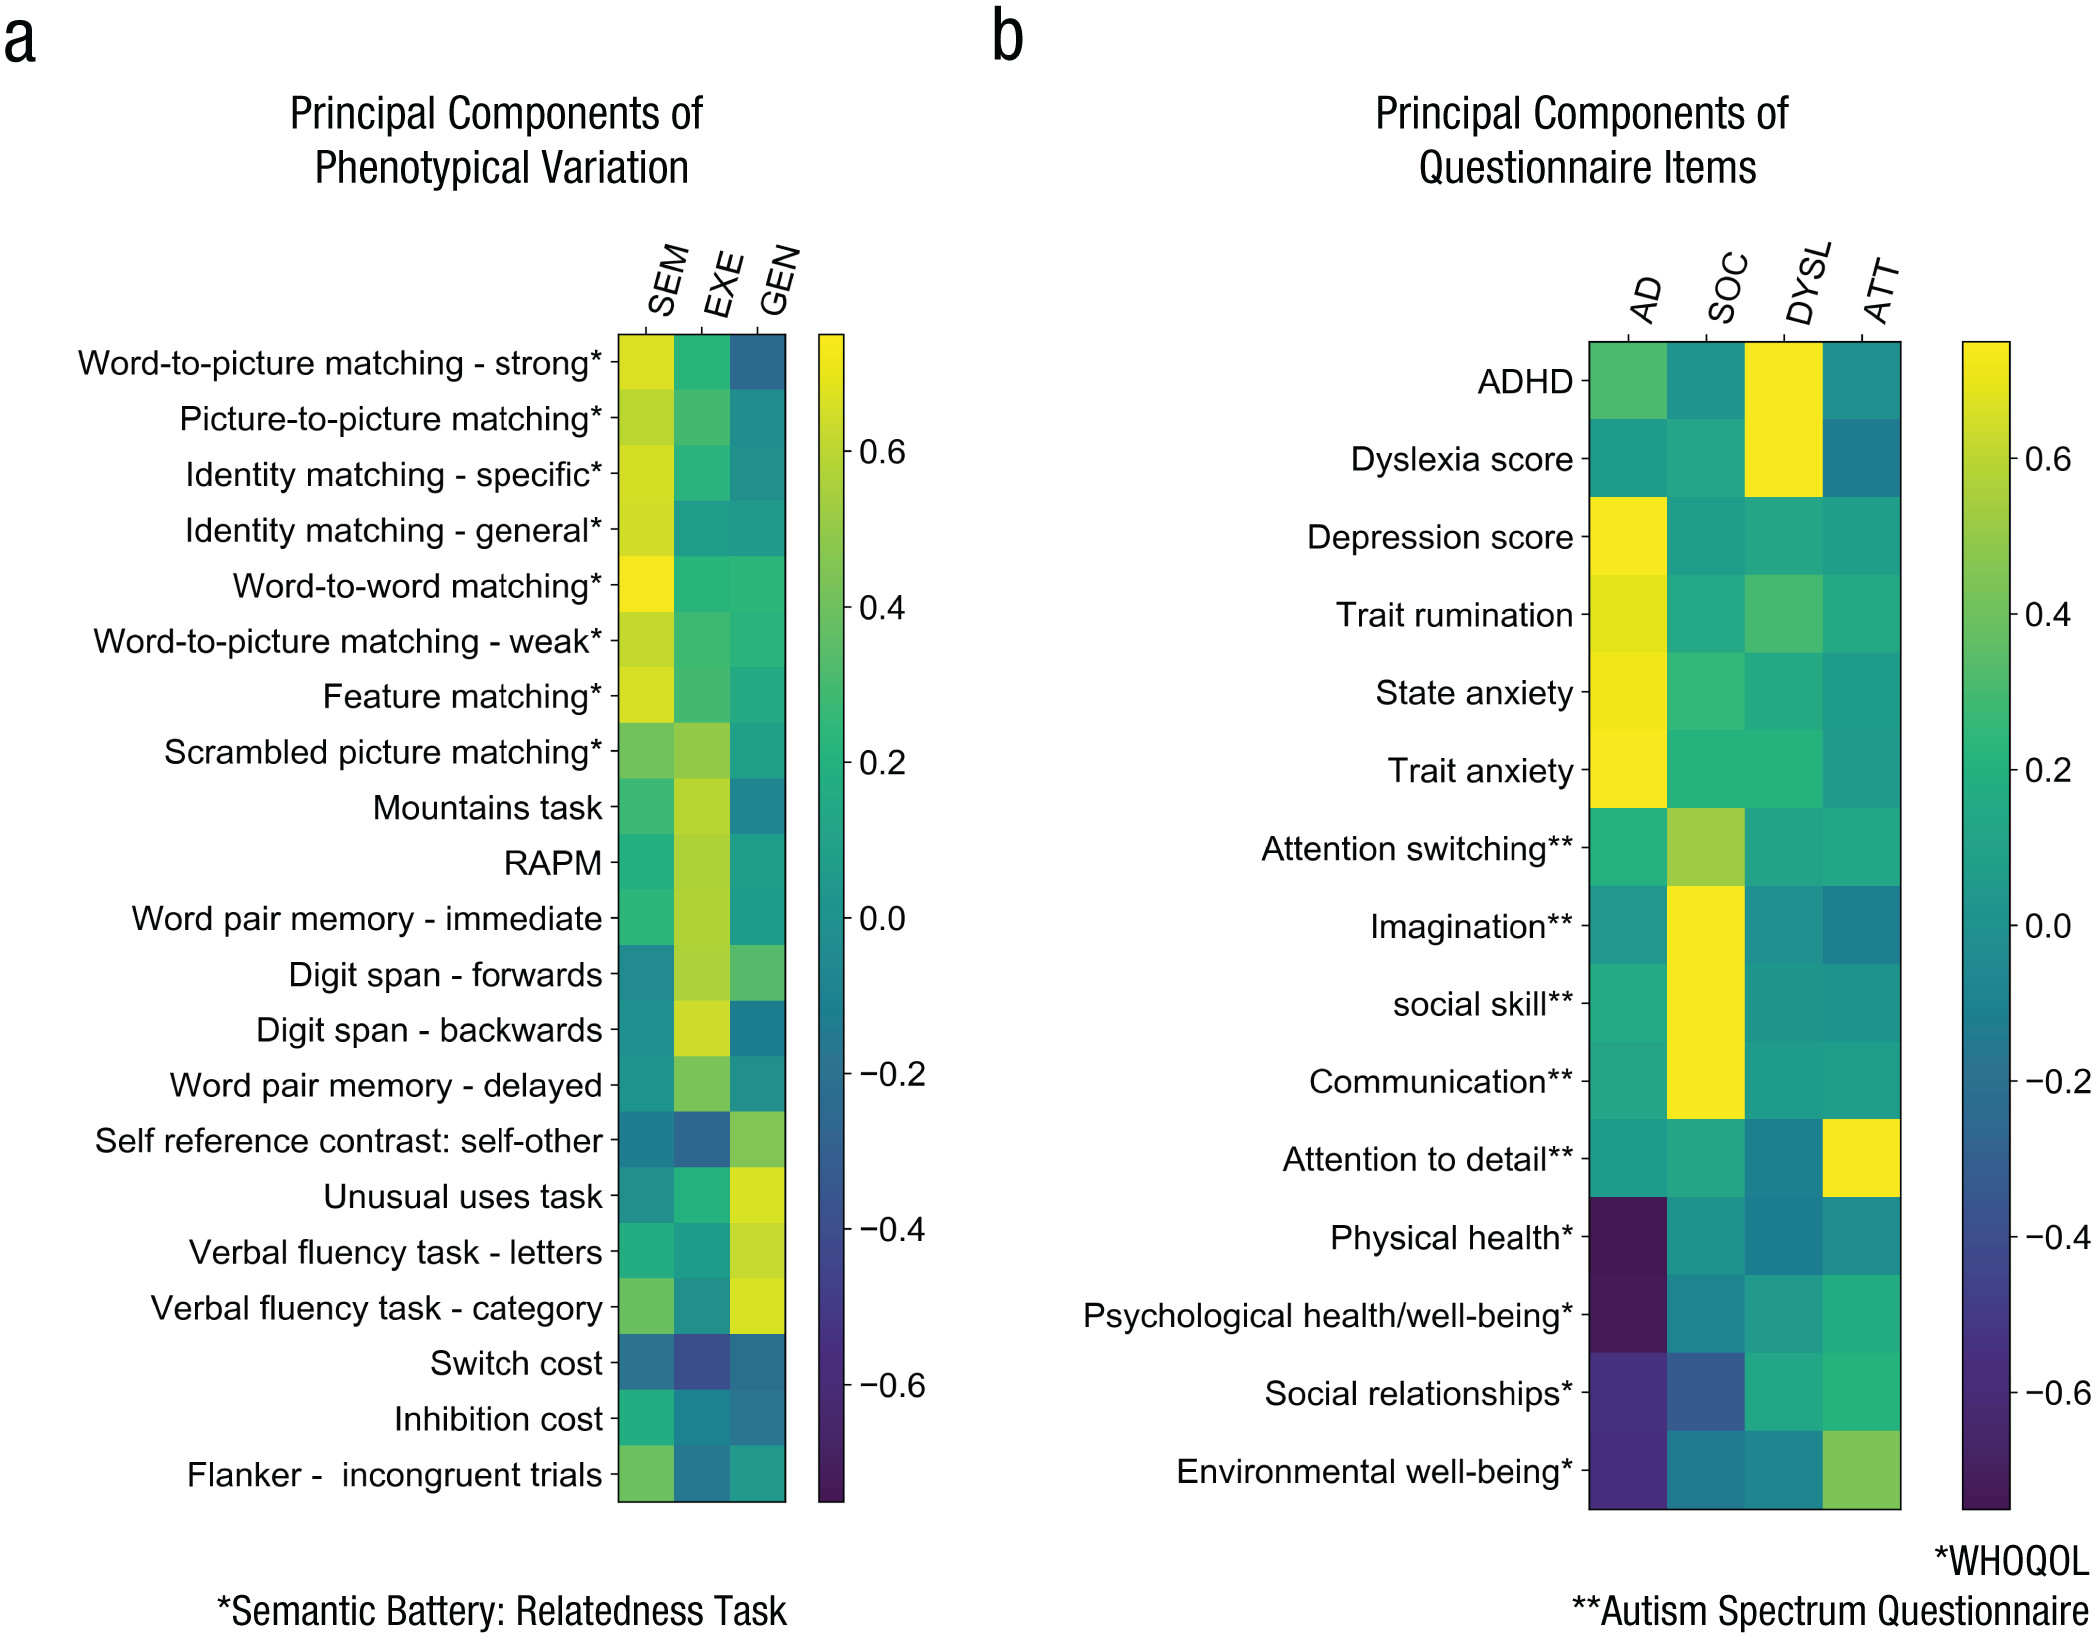
\includegraphics[width=0.8\textwidth]{study1/image/study1fig3.jpeg}
	\caption{Results from principal component analyses of (a) behavioural tasks and (b) questionnaires.}
	\caption*{\footnotesize{In the analysis of behavioural tasks, the components were semantic memory (SEM), executive control (EXE), and the generation of information (GEN). In the analysis of questionnaire data, the components were affective disturbance (AD), social interaction (SOC), dyslexia (DYSL), and attention to detail (ATT). The heat map indicates the loadings of each measure. In (a), an asterisk indicates that measures were relatedness tasks from a semantic battery. In (b), a single asterisk indicates measures drawn from the World Health Organization Quality of Life assessment \cite{WHOQOL2002}, and two asterisks indicate measures drawn from the Autism Spectrum Quotient \cite{Baron-Cohen2001}. ADHD = attention-deficit/hyperactivity disorder; RAPM = Raven’s Advanced Progressive Matrices \cite{Raven1998}. For the scree plots describing the eigenvalues for each dimension, refer to \cref{fig:3S2} in \cref{appendix:study1:subsection3}.}}
	\label{fig:study1:fig3}
\end{figure}
% ==========================================================================================================

\section{Results}
\label{study1:results}

\subsection{Determining consistent categories of experience}
\label{study1:results:a}
We applied SCCA to the network-connection-strength values among ROIs in the DMN and the average scores on the experiential reports gained in the laboratory. We accepted 13 canonical components generated by SCCA (see \cref{fig:3S3} in \cref{appendix:study1:subsection3} for the complete set). Of these initial components, two were consistent when we randomly removed the MDES reports of 1 day per participant and when bootstrapping was used to provide a more comprehensive description of the sample (see \cref{study1:method}). The consistency of these patterns across the three different analyses indicates that, in qualitative terms, they were not unduly biased by a particular session of our study and were likely to provide adequate estimation of the population (\cref{fig:study1:fig2}b). These stable components are presented in \cref{fig:study1:fig2}b, in which we show both the bootstrapping results, the analysis that randomly excluded one session (restricted temporal sampling), and the common elements of each solutions.

Canonical Component 1 reflects a pattern of stronger coupling within the mPFC, as well as between the left inferior parietal cortex (subregion 2 in the TPJ; see \cref{fig:study1:fig2}a). This pattern of integration within key nodes of the DMN was associated with descriptions of experience as positive, evolving, and habitual. We will refer to this as \textit{positive-habitual} experiences. Canonical Component 2 was associated with relatively weak patterns of coupling between the pCC bilaterally (subregions 2 and 4 in the TPJ; see \cref{fig:study1:fig2}a) and regions of the mPFC (subregions 1, 5, and 6 in the vmPFC; see \cref{fig:study1:fig2}a). This component was associated with thoughts that were task unrelated and nondeliberate. We will refer to this component as \textit{spontaneous off-task} experiences.

\subsection{Validating the categories of experience}
\label{study1:results:b}
Having identified two reliable dimensions of neurocognitive experience, we tested whether these patterns accounted for additional variance in the measures that we collected in our experiment. We first conducted a whole-brain analysis to determine whether the different patterns of experience were associated with differential communication from the DMN to other areas of the brain. In this analysis, we first employed dual regression to calculate the subject-specific spatial maps describing the correlation of the DMN and the whole brain and then used these spatial maps as dependent measures in a group-level multiple regression in which participants’ variation in positive-habitual and spontaneous off-task experiences were both explanatory variables of interest (see \cref{study1:method}). This analysis revealed a pattern of regions in which connectivity was differentially related to the dimensions of \textit{positive-habitual} and \textit{spontaneous off-task} experiences. These regions were the left temporoparietal cortex, left hippocampus/entorhinal cortex, left lateral middle temporal gyrus, and the left pre-supplementary region. Extracting the connectivity in this network and plotting these against the different types of experience revealed that these regions showed a pattern of connectivity that was linked to the expression of positive-habitual experiences but was unrelated to levels of spontaneous off-task experiences. These data are consistent with those found in previous studies that show that medialtemporal connectivity with the DMN is linked to aspects of spontaneous experience, such as episodic thought \cite{Karapanagiotidis2017}, and on-line studies that show that activity in this region is important during mind-wandering states \cite<e.g.,>{Ellamil2016}. It also confirms theoretical accounts of states of mind wandering as relying on regions that fall outside of the core of the DMN, such as the pre-supplementary motor area \cite<pre-SMA;>{Christoff2016}.

\begin{sidewaysfigure}[p]
	\centering
	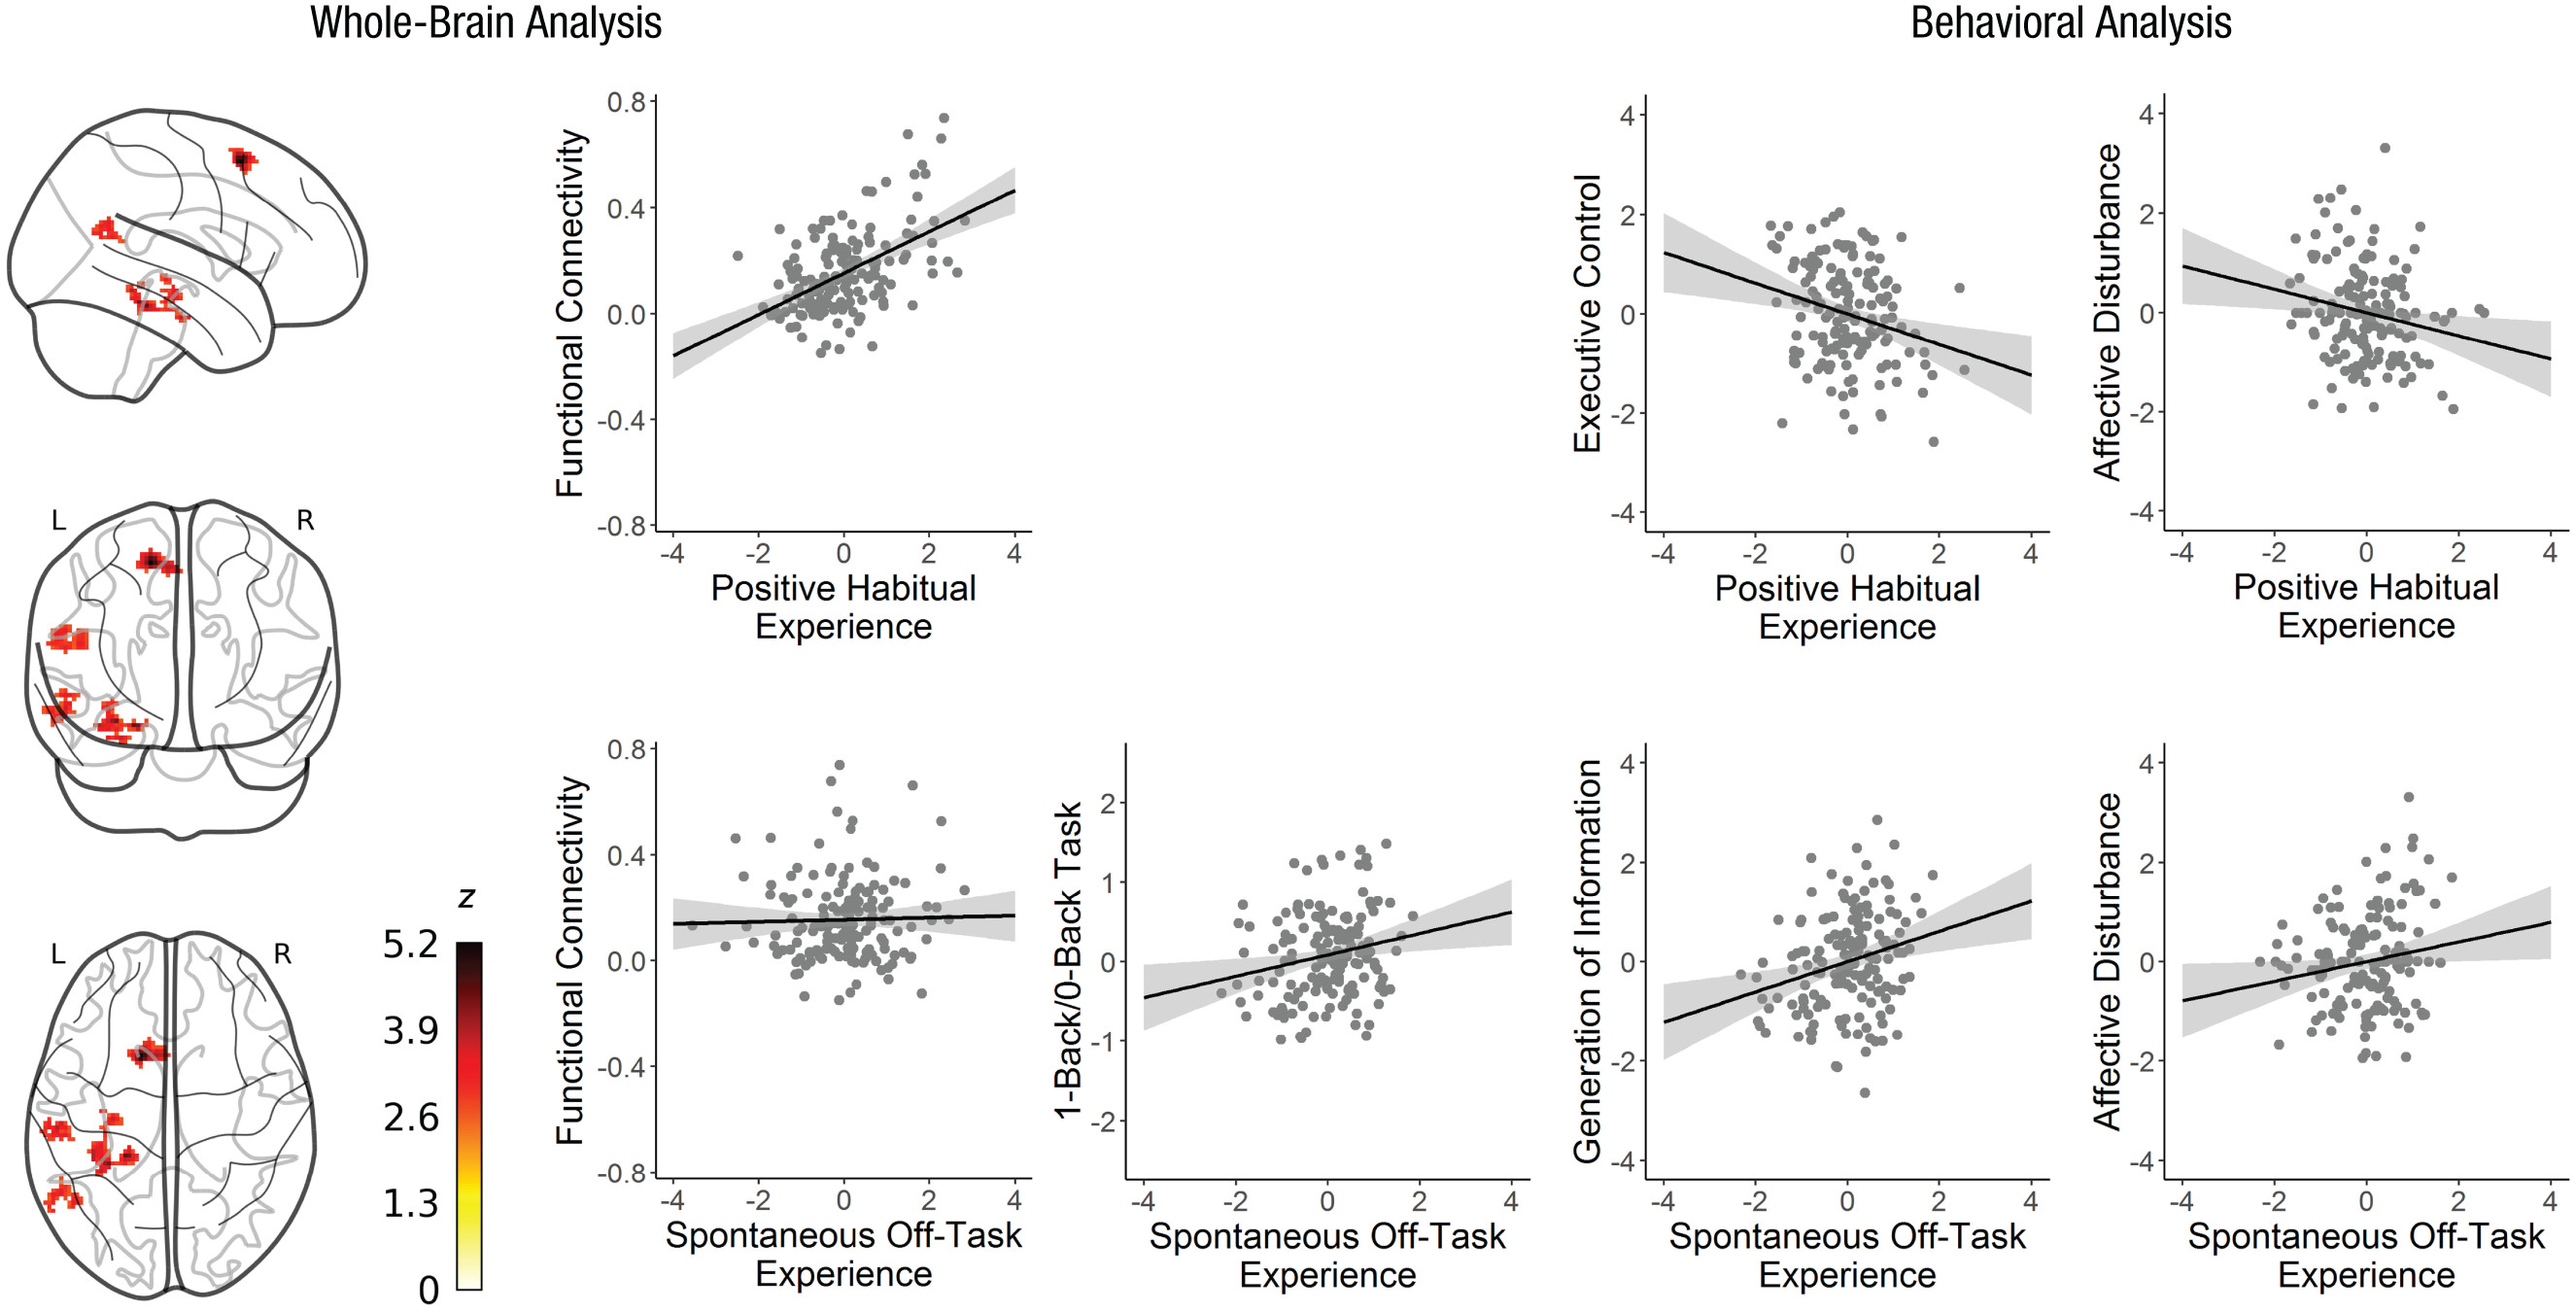
\includegraphics[width=0.8\textwidth]{study1/image/study1fig4.jpeg}
	\caption{Relationship between the different neural-cognitive components and the laboratory and questionnaire measures.}
	\caption*{For the whole-brain analysis, the brain diagrams show clusters of the default-mode-network mask, and the graphs show the correlation between their functional connectivity and the two experience components. For the behavioral analysis, the graphs show the relationship between the two canonical components and measures of well-being and task performance.}

	\label{fig:study1:fig4}
\end{sidewaysfigure}

Next, we explored whether the different canonical components had specific implications for performance on the tasks in which we assessed experience (i.e., the 0-back/1-back task). Because the SCCA depends on resting-state data recorded independently of the task, we were unable to estimate the canonical components separately for each task. Consequently, in these analyses, we explored whether overall differences in canonical component loadings across participants were associated with performance efficiency on the 0-back/ 1-back task. We used a repeated measures analysis of variance in which the dependent variable was the efficiency with which participants performed the 0-back/ 1-back task, respectively. This analysis revealed a significant interaction between task efficiency and variation in our spontaneous-off task component,
\(\mathit{F}(1, 154) = 6.43\),
\(\mathit{p} = .012\),
\(\mparetasquared = .04\).
Decomposition of this interaction showed that participants who scored higher on spontaneous off-task experience performed better on the 0-back condition,
\(\mathit{b} = 0.06\),
\(\text{95\% confidence interval (CI)} = [0.01, 0.11]\),
\(\mathit{t}(151) = 2.38\),
\(\mathit{p} = .019\),
\(\mparetasquared = .04\),
and worse on the 1-back condition,
\(\mathit{b} = -0.09\),
\(\text{95\% CI} = [-0.15, -0.02]\),
\(\mathit{t}(151) = -2.55\),
\(\mathit{p} = .012\),
\(\mparetasquared = .04.\)
The differential relationship between the levels of spontaneous off-task experience and performance on the 0-back/1-back task is shown in \cref{fig:study1:fig4}. These data confirm accounts that suggest that attentional lapses linked to mind wandering are context dependent, tending to have more negative effects as tasks become more demanding \cite{SmallwoodCC2013}; they are also consistent with prior studies suggesting that context regulation may be more problematic for spontaneous than deliberate mind wandering \cite<see also>{SeliTiCS2016}.

Finally, we used MANOVA to determine how the patterns of experience revealed by SCCA were related to the decompositions of the battery of cognitive performance and questionnaire measures. In this analysis, PCA scores describing either phenotypical variation or questionnaire measures on each of the components of cognitive function were the independent variables, and the individual loadings for each of the two canonical components describing experience from the SCCA were the dependent variables. For the analysis of phenotypical variation, this produced two significant results with the executive-control component,
\(\mathit{F}(2, 152) = 5.84\),
\(\mathit{p} = .006\),
\(\mparetasquared = .065\),
and the generation-of-information component,
\(\mathit{F}(2, 152) = 3.41\),
\(\mathit{p} = .007\),
\(\mparetasquared = .065\).
Higher loadings on the positive-habitual component,
\(\mathit{F}(1, 153) = 9.84\),
\(\mathit{p} = .002\),
\(\mparetasquared = .060\),
were associated with worse performance on tasks requiring executive control,
\(\mathit{b} = −0.19\),
\(\text{95\% CI} = [−0.32, −0.07]\),
\(\mathit{t}(153) = −3.14\),
\(\mathit{p} = .002\),
\(\mparetasquared = .060\),
and higher loadings on the spontaneous-off task experience component,
\(\mathit{F}(1, 153) = 10.15\),
\(\mathit{p} = .002\),
\(\mparetasquared = .062\),
were associated with better performance on tasks involving the generation of information (such as creativity),
\(\mathit{b} = 0.20\),
\(\text{95\% CI} = [0.08, 0.33]\),
\(\mathit{t}(153) = 3.19\),
\(\mathit{p} = .002\),
\(\mparetasquared = .062\).
This indicates that two of the experiential components identified by the SCCA were uniquely associated with poor performance on executively demanding tasks and better performance on measures of creativity: both aspects of psychological functioning that have previously been linked to mind wandering \cite<e.g.,>{Baird2012,McVay2009}. The relationships for both neurocognitive dimensions are shown in \cref{fig:study1:fig4}.

In terms of the relationship to the questionnaire decomposition, we found a significant association with the first principal component,
\(\mathit{F}(1, 151) = 3.76\),
\(\mathit{p} = .026\),
\(\mparetasquared = .05\),
which captured affective disturbance. This revealed two significant relationships: (a) a strong association with the positive-habitual component,
\(\mathit{F}(1, 152) = 6.13\),
\(\mathit{p} = .014\),
\(\mparetasquared = .04\),
which suggests a negative association between positive-habitual thought and levels of affective disturbance,
\(\mathit{b} = −0.16\),
\(\text{95\% CI} = [-0.29, 0.03]\),
\(\mathit{t}(152) = −2.48\),
\(\mathit{p} = .04\),
\(\mparetasquared = .062\),
and (b) an association with the spontaneous-off-task-experience component,
\(\mathit{F}(1, 152) = 4.55\),
\(\mathit{p} = .035\),
\(\mparetasquared = .03\),
which suggests that higher loadings on this component were associated with higher levels of affective disturbance,
\(\mathit{b} = 0.15\),
\(\text{95\% CI} = [0.11, 0.28]\),
\(\mathit{t}(152) = 2.13\),
\(\mathit{p} = .035\),
\(\mparetasquared = .03\).
This analysis demonstrates that the different canonical components have dissociable associations with respect to well-being, capturing aspects of the bidirectional relationship between the mind-wandering state and affective disturbance highlighted by prior research \cite<e.g.,>{Killingsworth2010,RubyPlos2013}. Importantly, our analysis demonstrates that the different canonical components have dissociable associations with respect to well-being, which shows that our method captured both elements of the apparently contradictory analysis linking the mind-wandering state to well-being that has been highlighted by prior research.

One concern with resting-state functional connectivity arises from the possibility that the connectivity matrices are unduly affected by individual differences in motion \cite{Power2014}. Consistent with this possibility, our results showed a correlation at the group level between the positive-habitual component,
\(\mathit{r}(155) = .363\),
\(\mathit{p} < .001\),
but not the spontaneous-off-task-experience component,
\(\mathit{r}(155) = −.097\),
\(\mathit{p} = .229\).
Hence, we assessed the contribution of this association to our results linking positive-habitual thought to our measured phenotypes. We performed a series of stepwise analyses to identify the contribution that motion made to the phenotypical associations with positive-habitual thought. In these analyses, the canonical component was the dependent variable. We entered the principal components describing cognition or well-being in the first step and Jenkinson’s mean FD in the second step. Including motion significantly improved the predictive value of the model for well-being--
Model 1:
\(\mathit{R}^{2} = .06\),
\(\mathit{F}(4, 152) = 2.21\),
\(\mathit{p} = .07\),
\(\mparetasquared = .06\);
Model 2:
\(\mathit{R}^{2} = .19\),
\(\mathit{F}(5, 151) = 6.95\),
\(\mathit{p} < .001\),
\(\mparetasquared = .19\);
model change:
\(\mathit{R}^{2} = .13\),
\(\mathit{F}(1, 151) = 24.51\),
\(\mathit{p} < .001\)
--as well as of the model for cognition:
Model 1:
\(\mathit{R}^{2} = .07\),
\(\mathit{F}(3, 153) = 3.92\),
\(\mathit{p} = .010\),
\(\mparetasquared = .07\);
Model 2:
\(\mathit{R}^{2} = .18\),
\(\mathit{F}(4, 152) = 8.22\),
\(\mathit{p} < .001\),
\(\mparetasquared = .18\);
model change:
\(\mathit{R}^{2} = .11\),
\(\mathit{F}(1, 152) = 19.65\),
\(\mathit{p} < .001\).
In the case of well-being, the explained variance of the affective disturbance component was not improved with the inclusion of motion--
Model 1: affective-disturbance
\(\beta = -0.20\),
\(\mathit{t}(152) = −2.48\),
\(\mathit{p} = .014\),
\(\mparetasquared = .04\),
\(\text{95\% CI} = [−0.29, −0.03]\);
Model 2: affective-disturbance
\(\beta = −0.20\),
\(\mathit{t}(151) = −2.59\),
\(\mathit{p} = .011\),
\(\mparetasquared = .05\),
\(\text{95\% CI} = [−0.28, −0.03]\),
Model 2: mean-FD
\(\beta = 0.36\),
\(\mathit{t}(151) = 4.94\),
\(\mathit{p} < .001\),
\(\mparetasquared = .14\),
\(\text{95\% CI} = [3.29, 7.67]\).
Thus, the relationship between affective disturbance and positive-habitual thought remained largely unchanged by the inclusion of motion as a nuisance variable. In the case of cognition, executive control accounted for less variance in the positive-habitual component when mean FD was included--
Model 1: executive-control
\(\beta = −0.24\),
\(\mathit{t}(153) = −3.14\),
\(\mathit{p} = .002\),
\(\mparetasquared = .06\),
\(\text{95\% CI} = [−0.32, −0.07]\);
Model 2: executive-control
\(\beta = −0.16\),
\(\mathit{t}(152) = −2.17\),
\(\mathit{p} = .032\),
\(\mparetasquared = .03\),
\(\text{95\% CI} = [−0.25, −0.01]\);
Model 2:
\(\beta = −0.34\),
\(\mathit{t}(152) = 4.43\),
\(\mathit{p} < .001\),
\(\mparetasquared = .11\),
\(\text{95\% CI} = [4.82, 12.56]\).

Unlike in the well-being analysis, motion explained a substantial amount of variance that was shared in the relationship between executive control and positive-habitual thought. To explore whether the positive-habitual component reflected an artefact of motion, we selected participants for whom movement greater than 0.2 mm occurred on less than 5\% of the resting-state data (\(\mathit{N}\) = 134) and reran the SCCA with the identical pipeline. This produced similar solutions for both positive-habitual and spontaneous off-task thought (see \cref{fig:3S4} in \cref{appendix:study1:subsection3}). Importantly, positive-habitual thought was not significantly correlated with motion,
\(\mathit{r}(132) = .10\),
\(\mathit{p} = .236\),
but was correlated with poor executive control,
\(\mathit{r}(155) = -.26\),
\(\mathit{p} = .001\)
(see \cref{tab:S1} in \cref{appendix:study1:subsection3} for the full set of correlations).
This final analysis shows that in a more restricted sample in which motion did not correlate with either latent component, we still observed a relationship between positive-habitual thought and poor executive control.

% ==========================================================================================================
\section{Discussion}
\label{study1:discussion}
Using multivariate pattern analysis, our study demonstrated that the content of the mind-wandering state is heterogeneous and confirmed hypotheses that different types of experience have differing functional associations \cite{SmallwoodCC2013}.
Using a novel analysis strategy, we simultaneously decomposed self-reports of experience with descriptions of neural organisation, revealing dimensions of experience with unique phenotypical associations: positive-habitual experiences and spontaneous off-task thoughts.

Poor executive control, a well-documented association of mind wandering \cite{McVay2009},
predicted variation in positive-habitual thoughts. This pattern of thinking was linked to coupling in the mPFC, a region important for assigning value to neural signals \cite{Roy2012}.
It is possible that deficits in executive control during mind wandering emerge because of problems in assigning value to an external task, a view supported by evidence that financial motivation limits the impact of mind wandering on performance \cite{MrazekJoEP2012}.
We found that spontaneous off-task experiences simultaneously underlie the association between mind wandering and tasks of creativity \cite{Baird2012},
as well as problems in performing tasks requiring continuous monitoring of external information. Finally, while positive-habitual experiences are linked to improved well-being, spontaneous off-task experiences are associated with increased affective disturbance, which captures the apparent contradiction that mind wandering can be associated with both negative \cite<e.g.,>{Killingsworth2010}
and positive \cite<e.g.,>{PoerioFrontiers2016}
emotional states. Together, these data provide the most convincing evidence to date that experience during mind wandering unfolds along a set of underlying dimensions and that these explain many of the phenotypical associations that have hitherto been associated with the mind-wandering state \cite{SmallwoodCC2013}.

Our study also demonstrates the complex contribution that the DMN makes to cognition. Strong DMN connectivity at rest was associated with an increased tendency for positive-habitual thoughts about the future, which corroborates previous research linking the DMN to mental time travel \cite{Karapanagiotidis2017,Schacter2007}. Participants also rated these experiences as habitual, a pattern that supports accounts of the role of the DMN in cognition as emphasising automatic influences during mind wandering \cite{Christoff2016}. Spontaneous off-task thoughts, in contrast, showed weaker integration between core DMN regions and were linked to poor performance in the 1-back condition, a context in which task performance depends on the DMN functioning as a coherent network \cite{Konishi2015}. More generally, we found that states of high connectivity within the DMN (positive-habitual thoughts) were associated with more functional coupling to regions outside of the core network—a key prediction of the view that activity within the DMN reflects the integration of information from across the cortex \cite{Margulies2016}.
It is important to note that our analysis shows that the behavior of the DMN at rest contains information about individual variation in the type of experiences that emerge during mind wandering. These data should not be taken as evidence that this system is exclusive in its role in mind wandering. Indeed, our whole-brain regression provides quantitative evidence that the interactions of the DMN with other regions, including those in the medial temporal lobe and the executive system (e.g., pre-SMA), are also important. In this way, our study supports recent theoretical perspectives \cite<e.g.,> {Christoff2016,Margulies2016},
as well as prior empirical results \cite<e.g.,>{Ellamil2016,Golchert2017,Smallwood2016}
highlighting that regions other than the DMN core are important for mind wandering.

There are a number of limitations of the current analysis. First, our study focused on describing mind wandering as a trait. Prior work has shown similarities between state and trait measures of mind wandering in terms of (a) neural processing (e.g., trait: \citeNP{Smallwood2016};  state: \citeNP{Christoff2009,StawarczykPlos2011})
and (b) psychological processes such as working capacity
(e.g., trait: \citeNP{McVay2009}; state: \citeNP{MrazekJoEP2012})
and happiness
(e.g., trait: \citeNP{RubyPlos2013}; state: \citeNP{Killingsworth2010}).
Nonetheless there are certain aspects of mind wandering that can be understood only by treating it as a state, such as its temporal features
\cite{Christoff2016}.
Second, our study measured mind wandering in the laboratory. Although there is a correspondence between mind wandering in laboratory and naturalistic settings \cite<e.g.,>{McVay2009},
its form and content may depend on the contexts in which the experience emerges. Consequently, our findings should be supplemented by studies examining the occurrence of different types of experience in ecologically valid settings. Finally, our study did not find evidence for links with tasks that rely on semantic memory or for links to psychological traits other than well-being. This may have been due to our selection of neural regions or from our selection of questions. Prior studies have linked regions in the temporal lobe to the contents of thought \cite<e.g.,>{Smallwood2016},
a pattern of data that is consistent with a role of the semantic system in spontaneous thought \cite{Binder2009}.
Other work has highlighted awareness of mind wandering as important in traits such as hyperactivity \cite{Franklin2017}.
We anticipate that extending the selected regions of the cortex and the aspects of experience measured may extend our understanding of the mind wandering state to encompass forms of semantic processing and additional psychological traits.

In closing, our study provides the strongest evidence to date that the mind-wandering state is heterogeneous in its content, neural basis, and functional associations. We describe two neurocognitive dimensions capturing associations with attentional lapses, creativity and well-being, confirming much of the research on mind wandering conducted over the last decade. However, we also provide an explanation for why scientific accounts of mind wandering have been dominated by controversy, such as its relationship to
happiness \cite{Killingsworth2010},
creativity \cite{Smeekens2016},
executive control \cite{McVay2009},
and the DMN \cite{Gilbert2007}.
Our data suggest that these debates emerge from an erroneous assumption that mind wandering is a unitary psychological construct, when it is in fact made up of distinct states with unique neural correlates and functional associations. This ontological uncertainty has led to artificial controversies that hinder the development of a mature science of internal experience. Although our findings do not capture the full range of experiential dimensions on which the mind can wander, they convincingly demonstrate that it is untenable to characterise mind wandering as a uniform experience. As a discipline, we must embrace methodologies and analytical techniques that capture the complex nature of internal experiences, allowing researchers to accurately determine the contribution that they make to people’s lives.

% ==========================================================================================================

\chapter{Population Variation in the Associations Between Large-Scale Networks and Experiences at Rest}
\chaptermark{Large-scale network and experiences}
\label{ch:study2}
%\setcounter{equation}{0}

% ==========================================================================================================

\textit{The following chapter has been adapted from: }Wang, H.-T., Bzdok, D., Margulies, D., Craddock, C., Milham, M., Jefferies, E., \& Smallwood, J.(2018). Patterns of thought: Population variation in the associations between large-scale network organisation and self-reported experiences at rest.
\textit{NeuroImage}, \textit{176} (1), 518--527. doi: \url{10.1016/j.neuroimage.2018.04.064} \footnote{
J. Smallwood, and H.-T. Wang designed the study. The data was provided from C. Cameron and M. Milham. The analysis pipeline was constructed by H.-T. Wang under the supervision of D. Bzdok and J. Smallwood. Data were analyzed by H.-T. Wang, under the supervision of D. Bzdok, J. Smallwood, and E. Jefferies. H.-T. Wang and J. Smallwood drafted the manuscript. D. Bzdok, D. Margulies and E. Jefferies provided critical input to the interpretations. All the authors approved the final version of the manuscript prior to submission.}

% ==========================================================================================================

\section{Abstract}
Contemporary cognitive neuroscience recognises unconstrained processing varies across individuals, describing variation in meaningful attributes, such as intelligence. It may also have links to patterns of ongoing experience. This study examined whether dimensions of population variation in different modes of unconstrained processing can be described by the associations between patterns of neural activity and self-reports of experience during the same period. We selected 258 individuals from a publicly available data set who had measures of resting-state functional magnetic resonance imaging, and self-reports of experience during the scan. We used machine learning to determine patterns of association between the neural and self-reported data, finding variation along four dimensions. `Purposeful' experiences were associated with lower connectivity---in particular default mode and limbic networks were less correlated with attention and sensorimotor networks. `Emotional' experiences were associated with higher connectivity, especially between limbic and ventral attention networks. Experiences focused on themes of `personal importance' were associated with reduced functional connectivity within attention and control systems. Finally, visual experiences were associated with stronger connectivity between visual and other networks, in particular the limbic system. Some of these patterns had contrasting links with cognitive function as assessed in a separate laboratory session---purposeful thinking was linked to greater intelligence and better abstract reasoning, while a focus on personal importance had the opposite relationship. Together these findings are consistent with an emerging literature on unconstrained states and also underlines that these states are heterogeneous, with distinct modes of population variation reflecting the interplay of different large-scale networks.

% ====================================================================================================================
\section{Introduction}
\label{study2:intro}
Unconstrained processing reflects important population level variation in measures of cognition, affect, and demographic \/ lifestyle factors. Psychological studies show that almost a third of ongoing thought is unconstrained by events in the here-and-now \cite{Killingsworth2010}
with important links to cognitive and affective processing \cite{Mooneyham2013}.
In neuroscience, metrics defined from the brain during wakeful rest, describe the organisation of neural function at both the micro and macro scale \cite{Glasser2016,Margulies2016}.
They also reflect individual differences in cognitive function \cite{Finn2015},
psychiatric conditions \cite{Nooner2012}
and demographic \/ lifestyle factors \cite{Smith2015}.
These findings establish unconstrained neurocognitive processing as a core element of human cognition, highlighting the need to formally understand the underlying neural architecture, and the associated patterns of experience.

One perspective on unconstrained processing emphasises the role of memory, with contributions of conceptual and episodic representations to ongoing thought \cite{Binder2009,Gusnard2001}.
Psychological studies have shown that patterns of unconstrained processing have links with memory retrieval, creativity and planning \cite{Baird2012,Leszczynski2017,Medea2016,Poerio2017}.
Such evidence raises the possibility that episodic representations anchored in the medial temporal lobe \cite{Moscovitch2016}
or conceptual representation anchored in anterior temporal lobe \cite{Lambon-Ralph2017}
contribute to ongoing thought \cite{Smallwood2016}.
It is hypothesised that these systems' contribution to unconstrained states may be linked to the ability for these regions to become functionally decoupled from systems more directly involved in action and perception, allowing them to operate in an offline manner \cite{SmallwoodCC2013}.
This process of decoupling may also be important in neural systems closely allied to those involved in memory – the default mode network \cite{Raichle2001}.
These regions of transmodal cortex are relatively distant in functional and structural space from systems involved in perception and action, potentially facilitating their role in stimulus independent aspects of cognition \cite{Buckner2013,Margulies2016,Mesulam1998}.
Together these \textit{representational} accounts of unconstrained processing highlight default mode and limbic networks as important candidate neural systems, especially when decoupled from systems directly involved in perception and action.

Alternative perspectives on unconstrained thought emerge from links between types of ongoing experience and problems maintaining a task relevant goal in mind. This \textit{executive-failure} view \cite{Kane2012,McVay2009}
takes as a starting point evidence that patterns of ongoing thought, such as the experience of mind-wandering, are linked to problems on tasks including sustained attention \cite{McVay2009}
and measures of general aptitude and executive control \cite{MrazekJoEP2012}.
Task-based neuroimaging investigations highlight a network of regions that increase their activity across many different task situations, so called multiple demand regions \cite{Duncan2010}. %(Duncan, 2010).
These regions broadly correspond to three well described intrinsic networks: ventral attention, dorsal attention, and frontal-parietal networks. Since these systems are important for the effective performance of many different tasks then dysregulation within these systems could reflect the hypothesised \textit{executive-failure} contribution to aspects of ongoing thought \cite{McVay2009,Weissman2006}.%(McVay \& Kane, 2010; Weissman, Roberts, Visscher, \& Woldorff, 2006).

Other aspects of unconstrained processing could reflect the importance of affective processes, or different modalities of processing. Ongoing thought is linked to mood state: Experimental inductions of mood \cite{SmallwoodEmotion2009,Smallwood2011}
%(Smallwood, Fitzgerald, Miles, \& Phillips, 2009; Smallwood \& O'Connor, 2011)
as well as natural fluctuations \cite{Poerio2013, RubyPlos2013}
%(Poerio, Totterdell, \& Miles, 2013; Ruby, Smallwood, Engen, \& Singer, 2013)
impact on ongoing thought. Contemporary accounts of emotional processing emphasise the role of limbic regions including the amygdala \cite{Bzdok2013,Lindquist2012}
%(Bzdok, Laird, Zilles, Fox, \& Eickhoff, 2013; Lindquist, Wager, Kober, Bliss-Moreau, \& Barrett, 2012)
and anterior aspects the insula \cite{Touroutoglou2012},
%(Touroutoglou, Hollenbeck, Dickerson, \& Barrett, 2012),
suggesting these regions may be important in determining affective aspects of ongoing thought. Psychological studies of ongoing thought also suggest that another important dimension of unconstrained processing may reflect the different modalities of processing \cite{Konishi2017,Smallwood2016}.
%(Konishi, Brown, Battaglini, \& Smallwood, 2017; Smallwood et al., 2016).
It has been shown, for example, that the visual system plays an important role in the expression of visual imagery \cite{Ganis2004,Kosslyn2001}.
%(Ganis, Thompson, \& Kosslyn, 2004; Kosslyn, Ganis, \& Thompson, 2001).
Recent work has extended this evidence to shown patterns of activity with visual regions are linked to the emergence of visual, non-verbal, elements of ongoing thought \cite{Raij2017}.
%(Raij \& Riekki, 2017).
It is also possible that sensorimotor processes may be implicated in language processing during unconstrained processing, given that a role for these regions in langauge processing extends beyond production \cite{Bzdok2016,Pulvermuller2010,Pulvermuller2010a}.
%(Bzdok et al., 2016; Pulvermuller, 2010; Pulvermuller \& Fadiga, 2010).

Our study aimed to identify patterns of intrinsic connectivity associated with different patterns of unconstrained states and examines their neurocognitive features from the perspectives outlined above. We used a large publicly available dataset, containing measures of resting-state functional magnetic resonance imaging (fMRI), and an accompanying self-report instrument describing cognition experienced during the resting state \cite{Gorgolewski2014,Nooner2012}. We previously explored the relationships between patterns of ongoing thought and measures of neural activity, such as the fractional amplitude of low frequency oscillations, as well as the regional homogeneity of neural activity, in a sub sample of this data set \cite{Gorgolewski2014}. In this study we focused on connectivity, we applied sparse canonical correlation analysis (SCCA) to obtain a conjoined decomposition of self-reports of experience with matrices of whole brain connectivity data. This analysis produces multivariate patterns that reflect dimensions of variation that are mutually constrained by both brain and experience. In this way we capitalise on the fact that self-reports of experience during scanning and descriptions of ongoing neural processing provide complementary descriptions of unconstrained cognition. Our analysis, therefore, helps define, at a population level, the shared links between brain patterns and different types of experience. Moreover, respecting the multivariate nature of brain and behaviour space, as our analysis does, can accommodate complex many-to-many relationships between patterns of connectivity and self-reports, and therefore is sensitive to the possibility of degeneracy in the underlying data. As a final validation step we established whether these neurocognitive dimensions are associated with performance on a battery of available cognitive tasks, including measures of executive control and intelligence.

We use the dimensions our analysis produces, and their links with cognitive function to evaluate the perspectives on unconstrained thought outlined earlier. \textit{Representational} accounts emphasise links with neural systems involved in memory, such as the limbic system, and regions of transmodal cortex, such as the default mode network. They highlight states with lower levels of functional communication between these regions and those more directly involved in external action. In contrast, \textit{executive-failure} accounts emphasise dysregulation in attention and control networks as contributing to patterns of ongoing thought that are linked to problems in domain general task performance. Affective accounts highlight limbic regions as important hubs in aspects of ongoing thoughts linked to emotion. Finally, modality specific influences on unconstrained thought may depend on information codes represented in regions that specialise in that particular type of information, such as a role of visual cortex in experiences dominated by images. Notably, some views lead to dissociable predictions with respect to cognitive performance. For example, executive-failure accounts predict patterns of thoughts linked to worse performance on measures of cognitive function, while representational accounts makes the opposite prediction.
% ==========================================================================================================

\section{Method}
\label{study2:method}

\subsection{Participants}
\label{study2:method:participants}
We analysed 258 participants (females = 162; age range 18 –- 55, \textit{M} = 34.97, \textit{SD} = 12.24) obtained from the enhanced Nathan Kline Institute-Rockland sample (NKI-RS;  \url{http://fcon_1000.projects.nitrc.org/indi/enhanced/}).
Full details of the acquisition of this sample can be found in \citeA{Nooner2012}.
We selected participants between 18 and 55 years old as our sample, this choice allowed us to maximise the cohesive nature of our sample.  All the participants have the MRI data and less than 5 missing data points among the selected assessments.

\subsection{Cognitive measures and questionnaires}
\label{study2:method:cog}
Based on prior studies examining the links between spontaneous thought and cognitive performance \cite<see>{Mooneyham2013}, %(see Mooneyham \& Schooler, 2013)
we selected established neuropsychological measures linked to executive control, abstract reasoning and intelligence. The measures included the Delis-Kaplan Executive Function System \cite<D-KEFS;>{Swanson2005},
Wechsler Abbreviated Scale of Intelligence \cite<WASI-II;>{Wechsler1999},
and Wechsler Individual Achievement Test-Second Edition Abbreviated \cite<WIAT-IIA;>{Wechsler2005}.
In D-KEFS we selected the tower test (move accuracy ratio), colour-word interference test (errors inhibition\(/\)switching), verbal fluency test (letter fluency \(-\) category fluency), design fluency test (design accuracy), trail making test (sequencing errors score \(+\) set-loss errors score \(+\) time-discontinue errors score), and the proverb test (a measure of abstract semantic reasoning). We used the rescaled score (\textit{M} = 10, \textit{SD} = 3) in our analysis. Tasks measures that reflected error rates (i.e. the colour-word interference test and trail making test) were reversed, so that high rescaled scores indicated better task performance. All the scores were transformed to z-scores.

\subsection{ongoing cognition measure}
\label{study2:method:NYCQ}
The New York Cognition Questionnaire (NYC-Q) is a self-report tool used to assess the thoughts experienced at rest \cite{Gorgolewski2014,Sanders2017}.
%(Gorgolewski et al., 2014; Sanders, Wang, Schooler, \& Smallwood, 2017).
It assesses thoughts and feelings experienced during the resting-state period. The first section contains 23 questions about the content of thought. These questions covers the temporal, social, emotional aspects of spontaneous thoughts that have been shown to be important by prior studies \cite<e.g.>{RubyPlos2013}.
Participants rated each question on a scale of 1 (Completely did not describe my thoughts) to 9 (Completely did describe my thoughts). The second section contains 8 questions about the forms thoughts take, capturing aspects of experience such as modality and detail associated with experience that prior studies suggest as important for spontaneous thoughts \cite{Smallwood2016}.
Participants rated each question on a scale of 1 (Completely did not characterise my experience) to 9 (Completely did characterise my experience).  In the current study we analysed the two sections together to provide single solutions that combined information on both the content form of experience. The full list of questions and the corresponding labels are presented in \cref{tab:study2:1}. The questionnaire was administrated once after the resting-state scan in order to assess experiences during the scanning session. For the full details of the NYC-Q, please refer to \citeA{Gorgolewski2014}.
We have placed the questionnaire measure used in this study along with an example self-report collection task on GitHub at the following address:
\url{https://github.com/htwangtw/restingstate_thoughtreports}.

\linespacesmall

\begin{table}
\centering
\caption{The New York Cognition Questionnaire (NYC-Q).}
\label{tab:study2:1}

\resizebox{\textwidth}{!}{
\begin{tabular}{ l l}
\toprule
Questions&Labels\\
\midrule
I thought about things I am currently worried about&Concerns\\
I thought about people I have just recently met&People\\
I thought of people I have known for a long time (friends)&Friend\\
I thought about members of my family&Family\\
I thought about an event that took place earlier today&Today - Past\\
I thought about an interaction I may possibly have in the future&Social - Future\\
I thought about an interaction with somebody that took place in the past&Social - Past\\
I thought about something that happened at a place very close to me&Near Location\\
I thought about something that made me feel guilty&Guilt\\
I thought about an event that may take place later today&Today - Plan\\
I thought about something that happened in the recent past (last couple of days but not today)&Recent Past\\
I thought about something that happened a long time ago in the past&Distant Past\\
I thought about something that made me angry&Anger\\
I thought about something that made me happy&Happiness\\
I thought about something that made me cheerful&Cheerfulness\\
I thought about something that made me calm&Calm\\
I thought about something that made me sad&Sadness\\
I thought about something that is important to me&Importance\\
I thought about something that could still happen today&Today - Future\\
I thought about something that may take place in the distant future&Distant Future\\
I thought about something that could take place in the near future (days or weeks but not today)&Near Future\\
I thought about personal worries&Worries\\
I thought about something that happened in a place far away from where I am now&Distant Location\\
In the form of images:&Image\\
In the form of words:&Words\\
Like an inner monologue or audiobook:&Monologue\\
Like a television program or film:&Film\\
Had a strong and consistent personal narrative:&Narrative\\
Had a clear sense of purpose:&Purpose\\
Vague and non-specific:&Vague\\
Fragmented and disjointed:&Fragment\\
\bottomrule
\end{tabular}
}
\end{table}

\linespacenormal
\subsection{MR data processing}
\label{study2:method:MRI}

\subsubsection{Resting-state fMRI}
We used resting-state fMRI to describe the general functional organisation of the brain. We selected resting-state multiband functional magnetic resonance imaging (R-mfMRI;  TR = 1400msec; voxel size = 2mm isotropic; duration = 10 minutes) for our analysis. Functional and structural data were pre-processed using Configurable Pipeline for the Analysis of Connectomes (C-PAC; \url{https://fcp-indi.github.io/}) to interface with FMRIB’s Software Library (FSL version 5.0, \url{www.fmrib.ox.ac.uk/fsl}). Individual FLAIR and T1 weighted structural brain images were extracted using Brain Extraction Tool (BET). Structural images were linearly registered to the MNI-152 template using FMRIB's Linear Image Registration Tool (FLIRT). The resting-state functional data were pre-processed and analysed using the FMRI Expert Analysis Tool (FEAT). X, Y, Z displacement and the three axis rotations were used to calculate the mean frame displacement (FD), characterising movement of each participant during the scanning session (Power et al., 2014). Mean of the absolute values for FD were later used to account for subject specific head motion. No global signal regression was applied. The individual subject analysis involved: motion correction using MCFLIRT; slice-timing correction using Fourier space time series phase-shifting; spatial smoothing using a Gaussian kernel of FWHM 6 mm; bandpass filtering (0.1 Hz $<$ f $<$ 0.009 Hz); six motion parameters (as estimated by MCFLIRT) regressed out; cerebrospinal fluid and white matter signal regressed out (top five PCA components, CompCor method).

\subsubsection{Connectivity matrices}

To describe the functional architecture of the whole brain, we transformed the resting-state BOLD time series into connection strength values of the different networks for each participant. The whole brain parcellation was obtained from connectivity-based functional parcellation created by Yeo and collegues \citeyear{Yeo2011}.
The 7 network parcellation was used in the current study. We split the networks into two hemispheres and extracted clusters. Two voxels are considered connected only if they are adjacent within the same x, y, or z direction. This yielded 57 clusters from the Yeo 7 networks parcellation. The implementation of spatial clusters extraction was retrieved from python library Nilearn \cite[\url{http://nilearn.github.io/}, version 0.3.1]{Abraham2014}
Next, we extracted and then averaged the time series of all voxels within each cluster to create a cluster specific time series. We used these time series to create region-to-region symmetrical correlation matrices representing the correlations of the network signal that was computed for all the individual subjects. The off-diagonal of each correlation matrix contained 1596 unique region-region connection strengths (i.e., the upper or lower triangle of the network covariance matrix). This approach provided a measure of connection strength of the whole brain for each participant. Finally, Fisher’s r-to-z transformation was applied to each network covariance matrix.

\subsection{Conjoint decomposition of connectivity and experience}
\label{study2:method:ML}

\subsubsection{Decomposition methods}
\label{study2:method:ML:CCA}
We performed a sparse canonical correlation analysis \cite<SCCA; see>{Hastie2015}
on the functional connectomes and the NYC-Q reports, to yield latent components that reflect multivariate patterns across neural organisation and experience \cite<For similar application, see>{WangPsychScience2018}.
SCCA maximised the linear correlation between the low-rank projections of two sets of multivariate data sets with sparse model to regularise the decomposition solutions a process that helps maximise the interpretability of the results. The regularisation function of choice is L1 penalty, which produces 'sparse' coefficients, meaning that the canonical vectors (i.e., translating from full variables to a data matrix's low-rank components of variation) will contain a number of exactly zero elements. L1 regularisation conducted (i) feature selection (i.e., select only relevant components) and (ii) model estimation (i.e., determine what combination of components best disentangles the neurocognitive relationship) in an identical process. This way we handle adverse behaviours of classical linear models in high-dimensional data. A reliable and robust open-source implementation of the SCCA method was retrieved as R package from CRAN
\cite<PMA, penalized multivariate analysis, version 1.0.9>{Witten2009}.
The amount of L1 penalty for the functional connectomes and the NYC-Q reports were chosen by cross-validation. The procedure is described below.

\subsubsection{Model selection}
\label{study2:method:ML:model}
We employed cross-validation (CV) to select the most useful model across population samples and avoid overfitting \cite{BzdokYeo2017}.
The amount of the two L\textsubscript{1} penalty terms for the functional connectomes and the NYC-Q reports, respectively, were chosen by a nested K-fold CV, where the coefficient for the penalty were chosen using a grid search to maximise the quality of CV objective metric. The objective metric of choice was cumulative explained variances. The explained variance of each latent component was calculated using the squared canonical correlation. High explained variance suggests a high pattern recovery rate between the two data set. The sparse assumption is fundamentally in conflict with the statistical goal of finding components with high explained variance. Therefore we decided the number of components in the model before searching for the best parameter.

We performed confound removal on functional connectomes and the NYC-Q reports as suggested by prior studies \cite{Smith2015}.
We removed the effects of nuisance variables from the dataset. These confound variables were sex, age, and head motion indicated by Jenkinson’s mean FD \cite{Jenkinson2002}.
The removal steps was performed on the training set in each CV fold. We standardized the confound by calculating the z-score, and also squared the three confound measures to account for potentially nonlinear effects of these confounds. The 6 resulting confounds were regressed out of both data matrices. The implementation of the confound removal method \cite{Friston1994}
was retrieved from python library Nilearn \cite[\url{http://nilearn.github.io/}, version 0.3.1]{Abraham2014}.

\begin{figure}
	\centering
	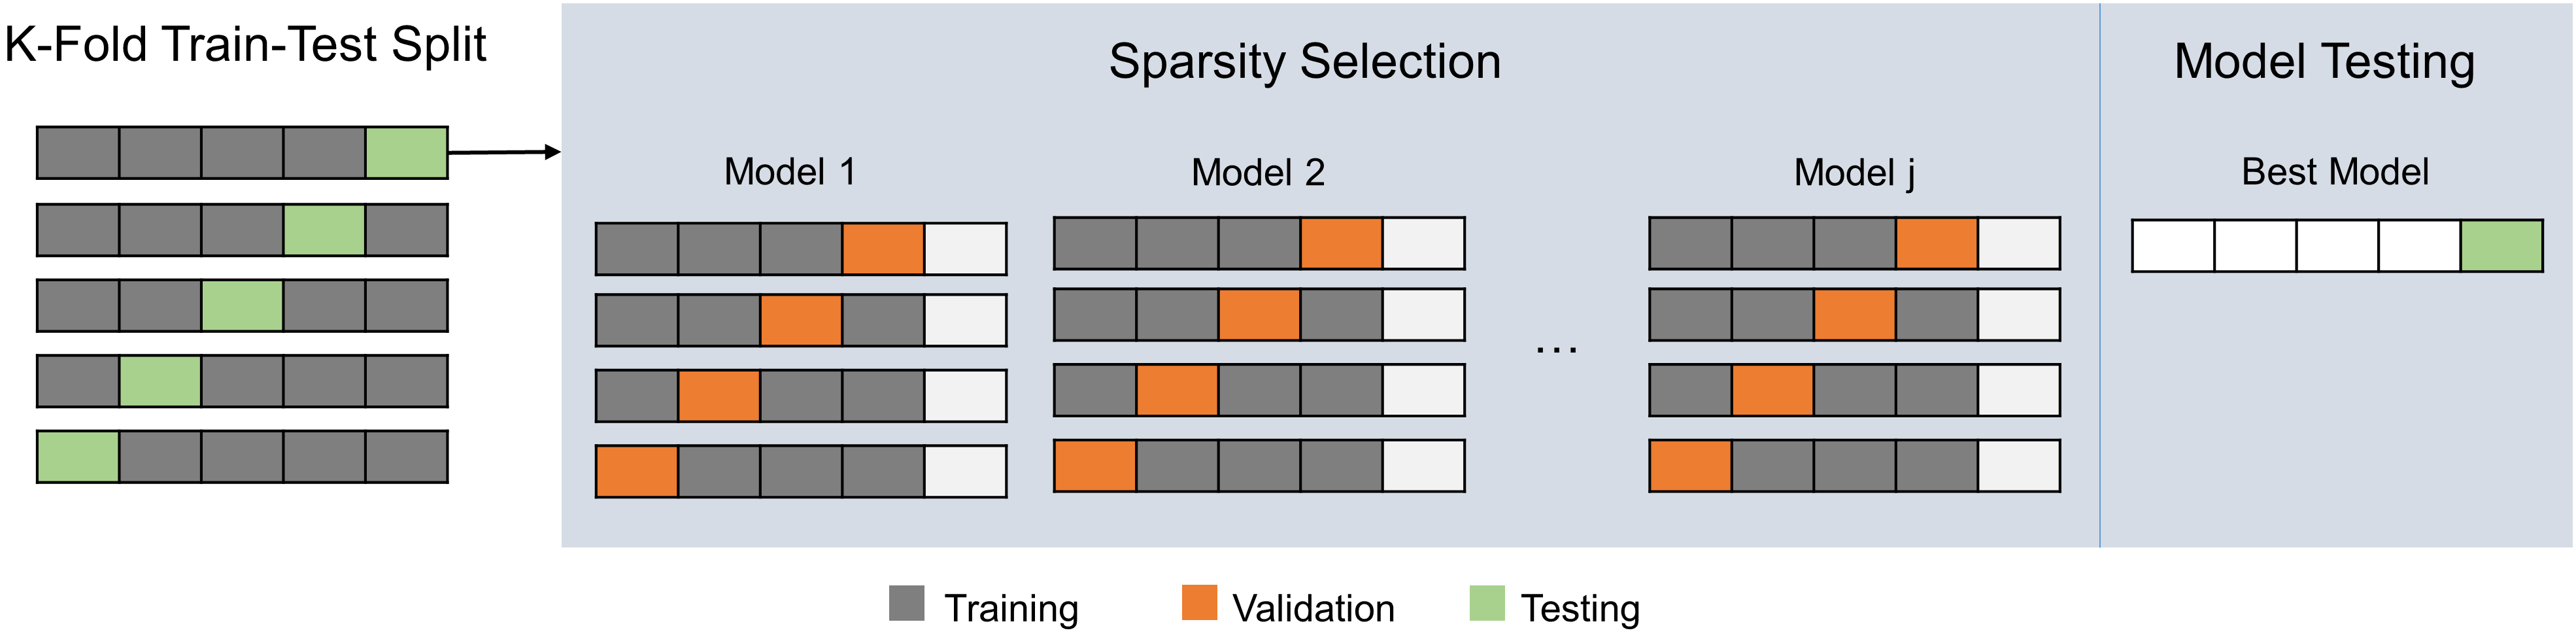
\includegraphics[width=0.8\textwidth]{study2/image/study2fig1.png}
	\caption{A diagram of the nested k-fold cross-validation with model selection.}
	\label{fig:study2:fig1}
\end{figure}

The number of latent components was determined by a preliminary analysis with no sparsity and calculated the explained variances for the two datasets (i.e., brain network correlations and questionnaire ratings). The explained variance increased with the number of components and growth stabilised at 10 components. We selected the number of components based on the point where the tangent stabilised. This led to a model of  4 components, and it accounted for a total of 78\% of the variance in connection strength and 29\% of the variance in the self-report data. Next, we determined the two coefficients for the L\textsubscript{1} penalty terms that was associated with the best model performance with 4 latent components. We searched for the best L\textsubscript{1} penalty values between 0.1 and 0.9 in 0.1 increments, which resulted in 81 set of parameters. For the nested K-Fold CV, we first separate the data into 5 consecutive folds after shuffling the data and retained one fold as the evaluation set (\(\mathit{N}\approx 50\)); the other four folds were used as the development set. The development set was further separated into 5 folds for parameter selection and each fold (\(\mathit{N}\approx 40\)) was used as the validation set once. The model was estimated on the training folds with all parameter sets, and after completion, we trained the model with the winning parameter on the whole development set and the finally tested the performance on the independent, unseen evaluation set. We selected the final parameters according to the best performance on the evaluation set across all folds of the outer CV loop (\cref{fig:study2:fig1}). This parameter set is used to train on the full development set and tested on the evaluation set. The parameter grid search and k-fold CV was conducted by the implementation in a Python library scikit-learn \cite<\url{http://scikit-learn.org/stable/}, version 0.18.2>{scikit-learn}.
The detailed algorithm for selecting the penalty values are presented in  \cref{appendix:kfold}: Nested K-Fold CV.

The model with the best test performance was selected as the final model. The final model’s sparsity coefficient are 0.8 (functional connectivity) and 0.5 (self-reports), and the out-of-sample explained variance was 48\%. We used the ensuing canonical vectors of the winning SCCA model to compute the latent component scores. There are two sets of canonical scores in a latent component, a weighted sum of variables forms the canonical vectors. For each latent component, we averaged the z-score of the canonical scores of the connection strength and NYC-Q as the combined scores. These scores described the summary of the experience with both the neural basis and the content reports.

\subsection{Test of component robustness}
\label{study2:method:robust}
After identifying the well performed components in compressing the brain-experience data, we examined the robustness of the four components in two different ways. The permutation test is a purely data-driven strategy that access the chance of discovering components in null samples. We also leveraged the brain-experience components to explain the cognitive functions, so that we can identify meaningful patterns by well-established cognitive measurements.

\subsubsection{Permutation test}
\label{study2:method:permute}
We used permutation testing to assess the robustness of the components identified through our analysis. We constructed a null distribution for each canonical component by holding the functional connectivity data in place and randomising the subject-wise order of self-reports data. This permutation scheme broke the link of individual differences in the dataset, therefore testing the robustness of the components in the hypothetical population. By calculating the false-discovery rate in the null distribution, we can conclude the possibility of discovering our components by chance with the given penalty coefficients. Hypotheses that are accepted with a 5\% level of significance. In the current analyses we adopt the permutation test with the FWE-corrected p-value by \citeA{Smith2015}
with data argumentation to increase the size of the resampling datasets to 1000. The four components were compared to the first sparse canonical correlation of the permuted sample. The low-rank components are more relevant that the rest, therefore we yield more conservative p-value by comparing to the first canonical correlation only. We performed 5000 permutation tests to get enough estimates for 4 decimal places.

\subsubsection{Group analysis}
\label{study2:method:manova}
To determine how patterns of unconstrained neurocognitive activity related to performance on the battery of cognitive tests, we conducted an independent statistical analysis on the identical subjects. A Type III multivariate multiple regression with Pillai's trace test was applied to 4 individual scores for each of the latent components describing experience from the SCCA  were the independent variables, and the original 8 measures of cognitive performance were the dependent variables that we hoped to described by the linear combination of the latent components. Pillai's trace test is considered to be the most powerful and robust statistic for general use \cite{Huberty2006}.
The p-values reported were based on Bonferroni correction. We also performed a principal components analysis (PCA) to identify the patterns of covariance among the 8 measures of cognitive performance and compressed the data. The relation between the principle score and the 4 brain-experience dimensions identified through SCCA was examined in a linear regression model with Pillai's trace test. The analysis was conducted in R (version 3.3.1).  The multivariate multiple regression was conducted in R (version 3.3.1) using function \texttt{Manova} in R package \texttt{car} (companion to applied regression, version 2.1-5).

\subsection{Code availability}
\label{study2:method:code}
The full analysis pipeline is freely available at \url{https://github.com/htwangtw/patterns-of-thought}.

% ==========================================================================================================

\section{Results}
\label{study2:results}

\subsection{Determining constituent category of experience}
\label{study2:results:cca}
We used Sparse Canonical Correlation Analysis (SCCA) to determine connectome-wide dimensions that describe common variance shared by descriptions of brain and experience. This took as input individual scores for the connections between each of the regions extracted from Yeo's 7 networks parcellation and the scores of each item of the New York Cognition Questionnaire (NYC-Q).

We applied SCCA with nested 5-fold CV as the model selection strategy. We obtained a model of 4 canonical components with penalty levels of 0.8 on the functional connectivity and 0.5 on the NYC-Q that indicated the best out-of-sample prediction on our data (see \cref{study2:method:ML:model}). The canonical correlations of the 4 latent components were 0.28, 0.19, 0.16, and 0.07. The latent components yielded by the best model are presented in \cref{fig:study2:fig2}. For the ease of presentation and interpretation, we summarised the components as network-network connectivity instead of 57-by-57 connectivity matrices. The heat maps describe the network-to-network correlations while the word clouds describe the loadings on the self-report items. The components in full and the heat map for the self-report items can be found in Online Supplementary Materials\footnote{Supplementary data related to this article can be found at \url{https://doi.org/10.1016/j.neuroimage.2018.04.064}}.

\begin{figure}
    \centering
    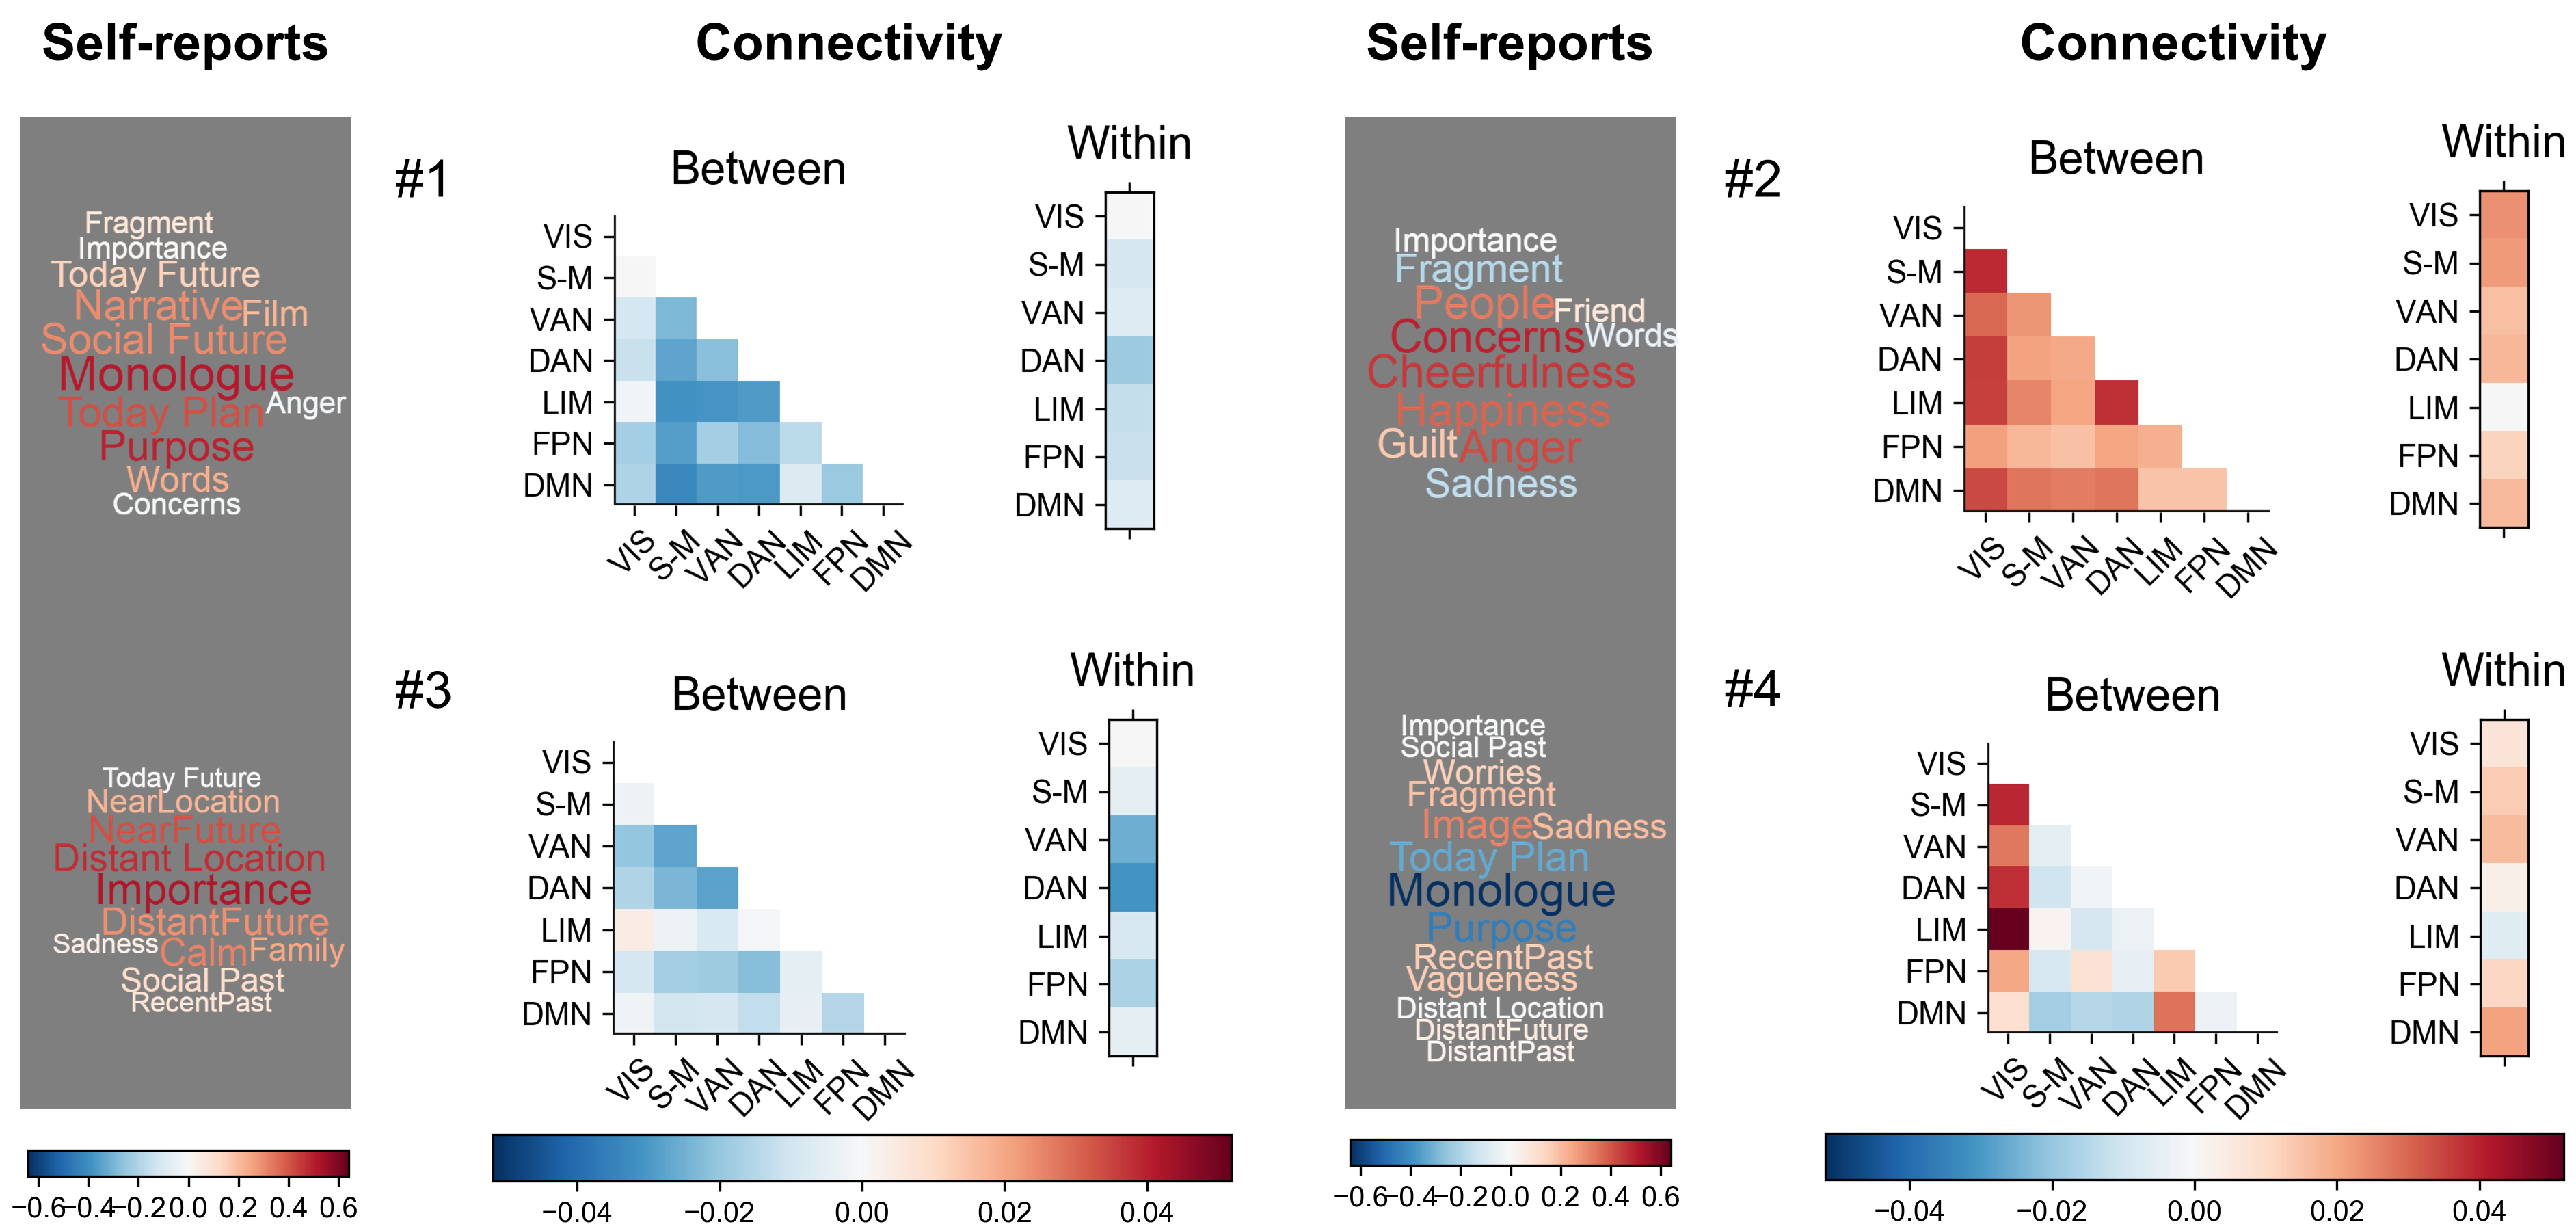
\includegraphics[width=0.8\textwidth]{study2/image/study2fig2.png}
    \caption{Unique neurocognitive dimensions of population variation revealed by sparse canonical correlation analysis of measures of whole brain connectivity and self-reported descriptions of ongoing experience.}
    \caption*{
    \footnotesize{
    The heat map describes the canonical variate of the network-to-network connectivity between different Yeo networks. The connectivity matrices describes the coefficients from the model, separated into within and between network relationships. The word clouds reflect the coefficients on the relevant self-report items. In both cases the colour bars indicate the magnitudes of the coefficients. A detailed version of the canonical variates and alternative presentation of the self-report coefficients can be found in  Online Supplementary Material Figure S1--S5
    }}
    \label{fig:study2:fig2}
\end{figure}

Component 1, describes patterns of reduced within network connectivity within all of the networks studied, with this pattern most prominent in the dorsal attention network. Between network connections are generally reduced, with the exception of visual to limbic. Sensorimotor was decoupled from all the other systems, and, in addition, the default and limbic were most decoupled from the attention networks. Experiential themes in Component 1 are dominated by themes related to deliberate planning with a verbal component (high loadings on `words', `monologue', `today-plan', `social-future', `purpose' and `deliberate'). We refer to this pattern of reports as reflecting thoughts with `purpose'.

Component 2 is dominated by relatively higher within and between network connections. Connectivity within each network was strong with the exception of the limbic network. Between network connections were stronger, with this pattern most apparent in the connections between limbic and ventral attention. In addition, the visual network was strongly correlated with the other networks. This component is dominated by emotional responses (high loadings on `anger', `guilt', `cheerfulness' and `happiness') and social content (`friends' and `people'). We refer to this pattern of reports as reflecting `emotional' experience.

Component 3 emphasises reduced connections both between and within networks. Within network connectivity is weakest for the dorsal and ventral attention networks. Edge-to-edge connections are low, with the ventral and dorsal attention and frontoparietal networks showing reduced correlations with each other as well as the visual and sensorimotor systems. This component was characterised by themes linked to personal `importance' with social temporal contents (`distant future', `near future', `social past', `family' and `recent past'). We refer to this pattern of reports as reflecting `personal importance'.

Component 4 has the most heterogeneous pattern of within and between network connectivity. It is associated with stronger connections within networks with the exception of the limbic system. In addition, the visual system was strongly connected to all other networks, with this pattern most apparent for the limbic network. In contrast, lower network-to-network connectivity was observed between the default mode and sensorimotor and attention networks. This component is characterised by experiential patterns reflecting a modality difference in experience, with the highest loadings on `images' and lowest on `inner monologue'. We refer to this pattern of reports as describing `modality'.


\subsection{The relationship between neuroexperiential components and cognitive functions}
\label{study2:results:manova}
Having documented four neurocognitive dimensions, we next examined the robustness of the components using two complementary approaches. We first used a permutation test to identify the chance of discovering components in null samples as employed by Smith and colleagues (2015). The top three components passed the permutation test and the \nth{4} component showed variance that was similar to that produced in a null sample
(Component 1: \(\mathit{p} = 0.0002\),
Component 2: \(\mathit{p} = 0.0010\),
Component 3: \(\mathit{p} = 0.0204\),
Component 4: \(\mathit{p} = 0.998\),
\(\alpha = 0.05\)).
This analysis suggests that Components 1--3 are unlikely to have occurred by chance. Component 4 may be a Type \rom{2} error and so we discuss this component in only a limited manner moving forward.
Our next test of the robustness of our components is whether they explained unique patterns of expertise in our battery of cognitive tasks. We used multiple multivariate regression model in which performance on the battery of selected tasks was the dependent variables and the individual scores for each of the canonical components describing experience from the SCCA were the independent variables. In this analysis two of the four canonical components described significant variance in our battery of tasks at multivariate level: 
Component 1 
(\(\mathit{F}(8, 246) = 2.21\),
\(\mathit{p} = .027\),
\(\mparetasquared = .067\))
 and Component 3 
(\(\mathit{F}(8, 246) = 2.56\),
\(\mathit{p} = .024\),
\(\mparetasquared = .068\)).

\begin{figure}[p]
    \centering
    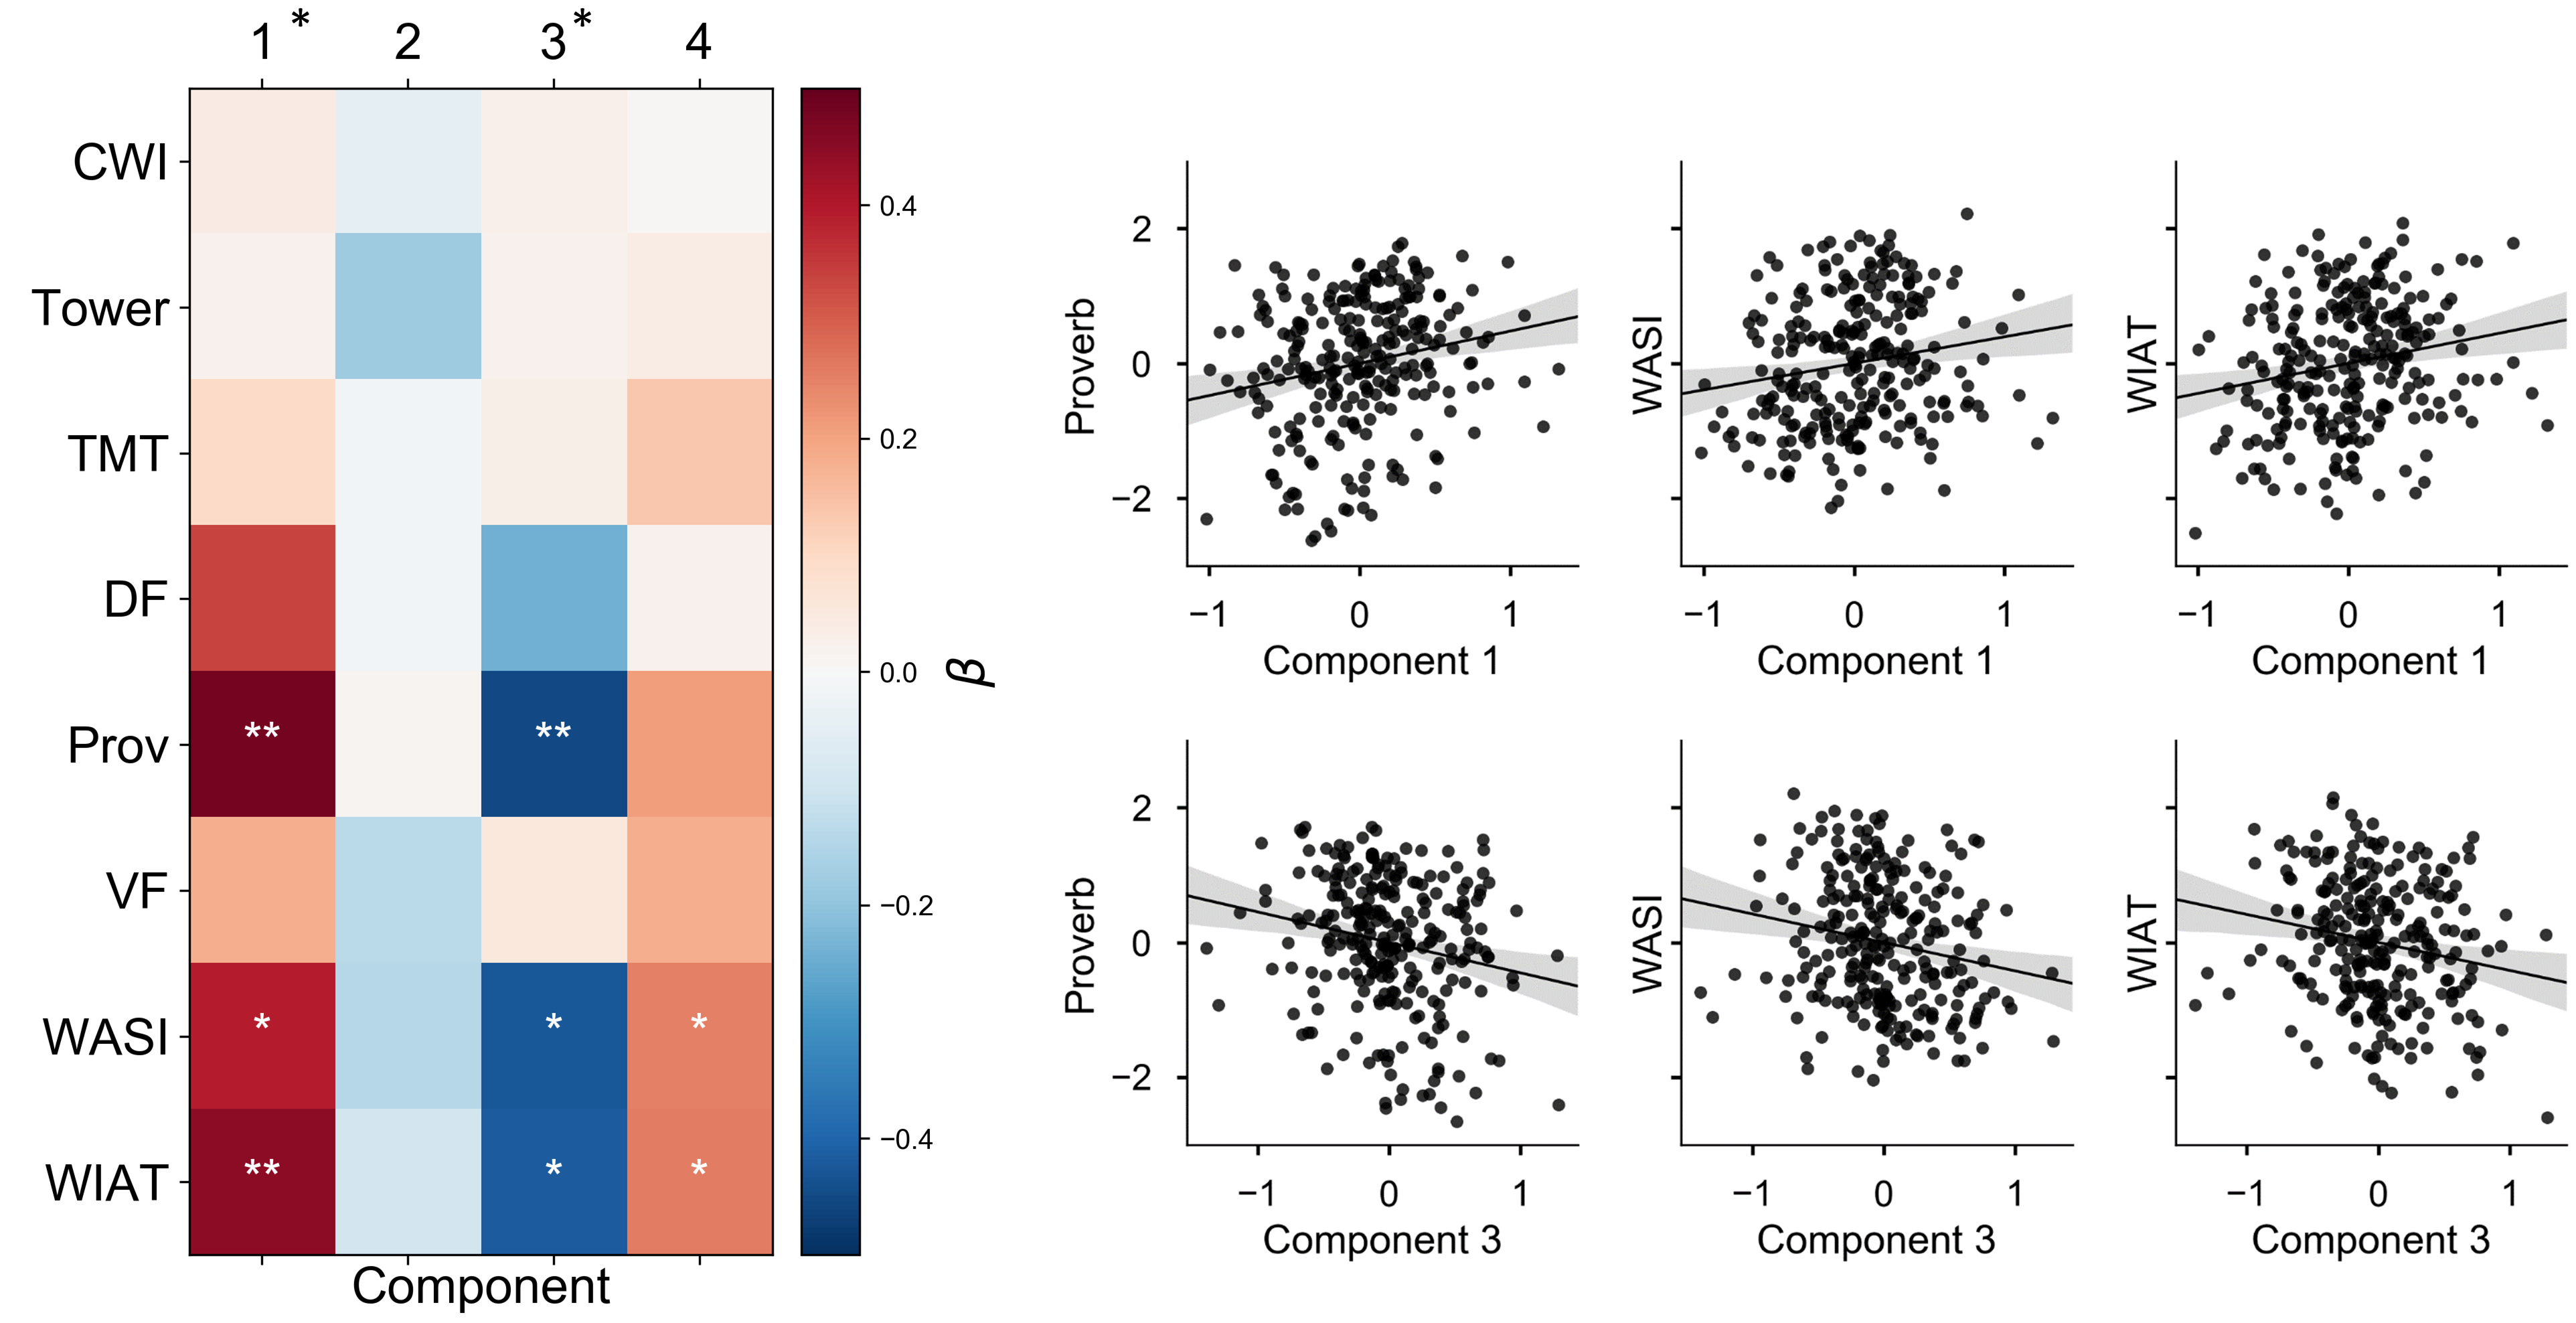
\includegraphics[width=0.7\textwidth]{study2/image/study2fig3.png}
    \caption{The relationship between the different neural-cognitive components and the measures assessed in the cognitive battery.}
    \caption*{
    \footnotesize{
    The components 1 and 3 were significant at the multivariate level determined by multiple multivariate regression, indicated by the asterisk outside of the heat map. The cells with asterisk(s) indicates the significant results from the univariate test (bonferroni corrected) and the parameter estimates for each variable. CWI: Colour-word interference, DF: Design fluency, Pro: Proverbs, TOW: Tower of London, TMT: Trail making task, VF: Verbal Fluency, WASI: Wechseler Adult Intelligence Test, WIAT: Weschler Individual Attainment Test. P-value significant codes:  0 `***' 0.001 `**' 0.01 `*' .}
    }
    \label{fig:study2:fig3}
\end{figure}

\begin{figure}[p]
    \centering
    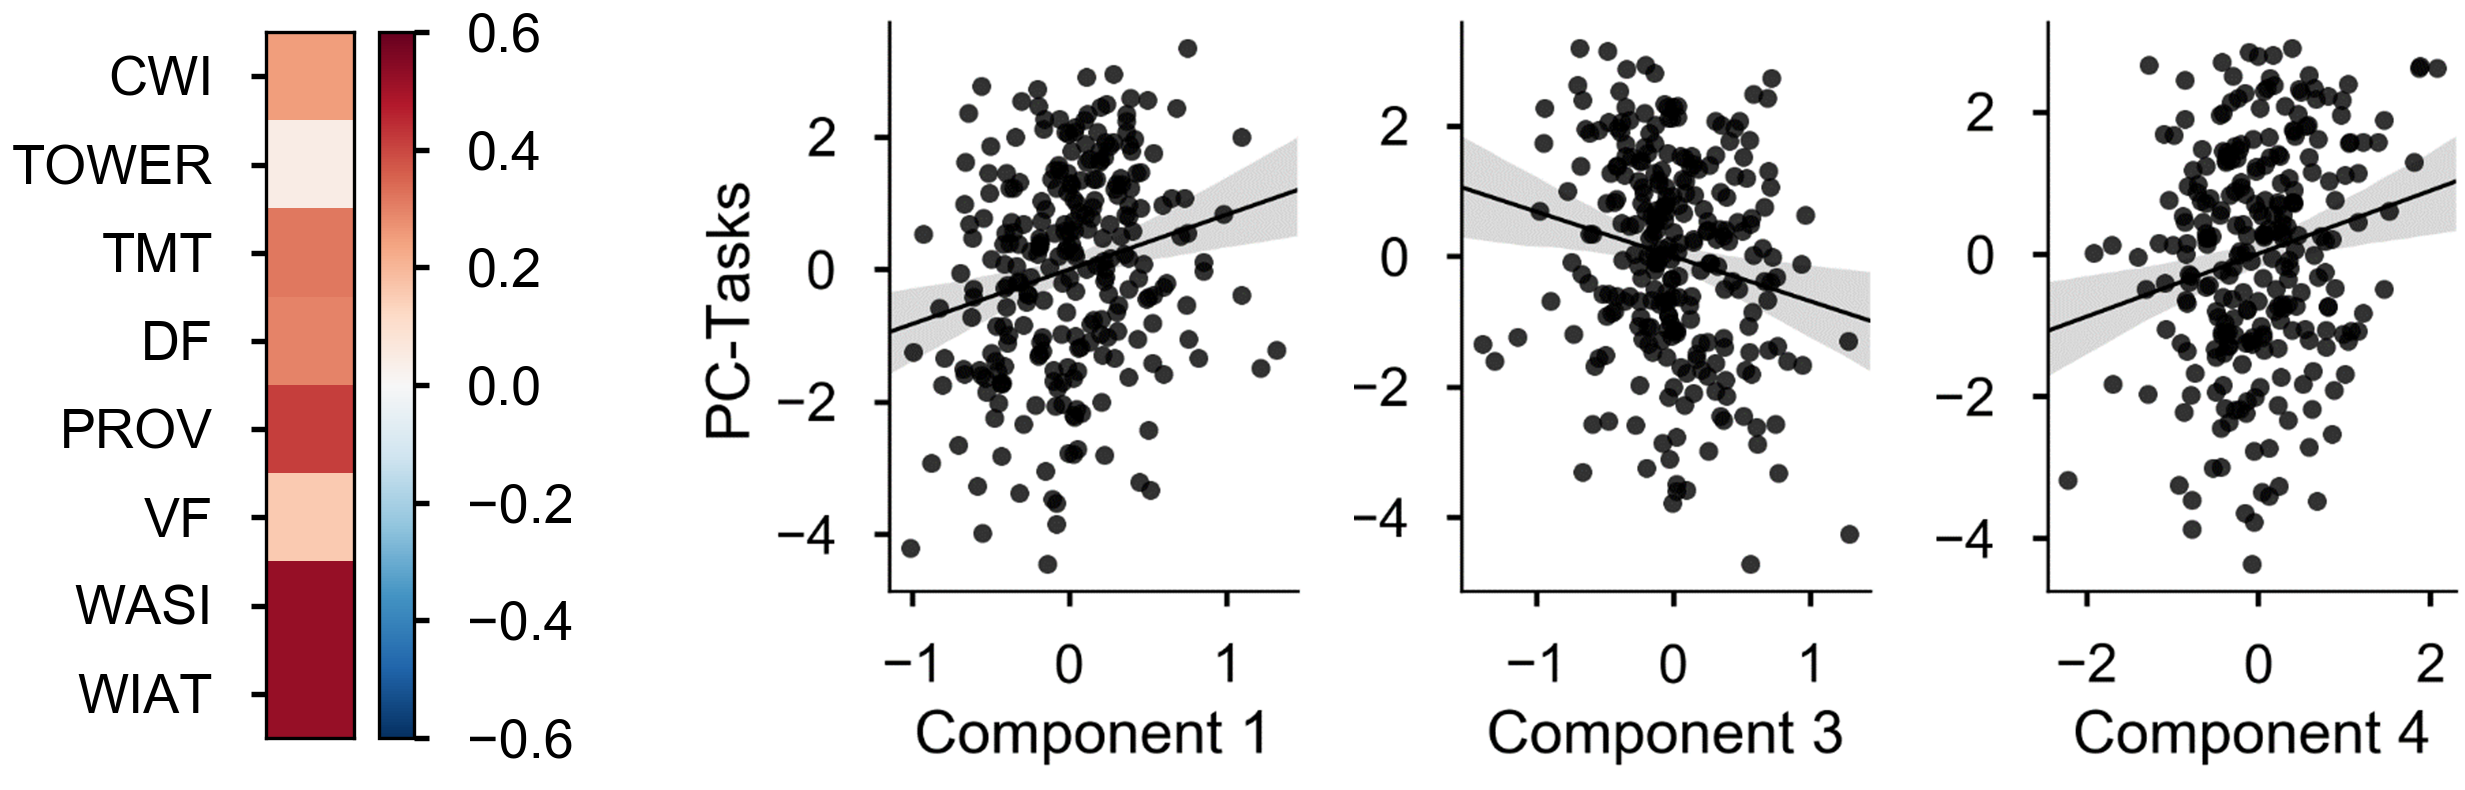
\includegraphics[width=0.7\textwidth]{study2/image/study2fig4.png}
    \caption{The principle component and its relationship to the different neurocognitive components.}
    \caption*{
    \footnotesize{The heat map describes the principle component of the task battery, and the scatter plots describe the association with the components identified in our study. Component 1 and 3 passed the permutation test for component robustness significantly contributed in explaining the principle component of the task. Component 4 showed a significant contribution in the regression model, but it did not pass the permutation test. The related results should be treated cautiously.}
    }
    \label{fig:study2:fig4}
\end{figure}

In the univariate results of the significant component, Component 1 was linked to good performance in proverb test 
(\(\mathit{b} = 0.48\),
\(\text{95\% CI} = [0.191  0.766]\),
\(\mathit{t}(251) = 3.27\),
\(\mathit{p} = .006\)) 
and both fluid intelligent tests WASI
(\(\mathit{b} = 0.39\),
\(\text{95\% CI} = [0.111 0.677]\),
\(\mathit{t}(251) = 2.74\),
\(\mathit{p} = .033\)) 
and WIAT
(\(\mathit{b} = 0.45\),
\(\text{95\% CI} = [0.167 0.724]\),
\(\mathit{t}(251) = 3.15\),
\(\mathit{p} = .009\)). Component 3 showed a reversed pattern of the cognitive functions related to Component 1: proverb test 
(\(\mathit{b} = -0.45\),
\(\text{95\% CI} = [-0.176 -0.727]\),
\(\mathit{t}(251) = -0.14\),
\(\mathit{p} = .007\)); WASI 
(\(\mathit{b} = -0.42\),
\(\text{95\% CI} = [-0.151 -0.693]\),
\(\mathit{t}(251) = -3.10\),
\(\mathit{p} = .012\)) and WIAT 
(\(\mathit{b} = -0.41\),
\(\text{95\% CI} = [-0.148 -0.682]\),
\(\mathit{t}(251) = -3.06\),
\(\mathit{p} = .012\)). 
The relationships between the neurocognitive dimensions and the pattern of relationships on the full cognitive battery and the adjusted variable scatter plots of the significant results are summarized in the form of a heat map in \cref{fig:study2:fig3}.

Finally, we performed a simple principle component analysis on the eight task measures to explore the associations between experience and the structure of the laboratory data. The aim of this analysis was to see if the pattern retrieved from the univariate level in the previous multiple multivariate regression was related to the internal structure of the data. Component selection was determined based on the scree plot, and we accepted one component explaining 39\% of the variance. The principle component loaded on the intelligence measures and the proverb test. We fitted a linear model to this data to understand the relationship to the four canonical components. The results are reported in \cref{fig:study2:fig4}. The overall linear model was significant 
(\(\mathit{F}(4, 253) = 5.43\),
\(\mathit{p} = .00003\)). In the linear regression model, Component 1 
(\(\mathit{b} = 0.82\),
\(\text{95\% CI} = [0.36 1.29]\),
\(\mathit{t}(253) = 3.5\),
\(\mathit{p} = .001\)) showed significant contribution to explaining the task principle component. Component 3 showed a negative correlation to the task components 
(\(\mathit{b} = -0.69\),
\(\text{95\% CI} = [-1.13 -0.24]\),
\(\mathit{t}(253) = -3.04\),
\(\mathit{p} = .003\)). The relationships between tasks and the neurocognitive components here were similar to the ones uncovered by the multiple multivariate regression. In this analysis Component 4 
(\(\mathit{b} = 0.442\),
\(\text{95\% CI} = [0.16 0.72]\),
\(\mathit{t}(253) = 3.09\),
\(\mathit{p} = .002\)) showed a significant contribution in the regression model, but it did not pass the permutation test of robustness (\(\mathit{p} = 0.998\)). The related results should be treated cautiously. Together with our prior analysis, these results suggest that Components 1 and 3 are the most robust components identified in our study.

% ==========================================================================================================

\section{Discussion}
\label{study2:discussion}
We set out to describe different modes of neurocognitive patterns derived through the simultaneous decomposition of whole brain connectivity data with self-reports of ongoing experience. We used a whole brain parcellation that describes cortical function in seven independent networks \cite{Yeo2011}.
We combined this data with self-reports of the experience of our participants at rest, using a multivariate approach that allows for the possibility of many-to-many mappings between neural patterns and ongoing cognition. Our analyses identified four stable canonical components, describing unique dimensions of neural-experiential variation. Permutation testing demonstrated the statistical robustness of Components 1-3. Furthermore, two components (1 and 3) described independent patterns of performance in a battery of commonly used cognitive measures. This association with cognitive performance that establishes a source of independent validity for these neurocognitive components since they are related to independent measures of cognitive performance. We next consider the fit between the dimensions produced by our analysis and theoretical views of unconstrained neurocognitive processing.

We found evidence broadly consistent with contemporary representational accounts of unconstrained processing. The neural patterns described by Component One reflect a pattern of reduced correlation between regions with links to memory and representation (e.g. limbic, default mode) from those with links to external behaviour (e.g. visual and sensorimotor cortex and attention networks). This pattern was associated with experiences characterised by a sense of purposefulness, and with verbally mediated content that was social and temporal in nature. Participants high on this dimension were proficient at generating abstract semantic links and performed well on measures of reasoning and intelligence. Together the features of Component One support the hypothesis that the functional decoupling of systems important for memory and representation are important for aspects of unconstrained cognition \cite{SmallwoodFrontiers2013}.
This capacity may arise from the topographical organisation of the cortex, in which neural systems that can take on more transmodal properties tend to be located in regions that are more distant in functional and structural terms \cite{Buckner2013,Margulies2016,Mesulam1998}.
This spatial location may allow neural signals in these regions to take on properties that are discrepant from the neural signal more closely tethered to inputs describing the external world \cite{Buckner2013,Friston2013}.
The pattern identified by Component One, therefore, may reflect a pattern of population variation describing the hypothesised role of functional decoupling of memory and representational systems plays in the generation of more abstract aspects of human cognition \cite{Margulies2016,Mesulam1998}.
Importantly, in our prior work, limbic and default mode networks were the most distant in functional connectivity terms from unimodal systems \cite{Margulies2016}.
Our data also highlights neural patterns that capture the hypothesised influence of attention and control on ongoing thought \cite{McVay2009}.
Component 3 highlights links between reduced connectivity within attention and control systems and patterns of thought that emphasise personal importance. This is associated with worse performance on measures of intelligence and reasoning. The combination of a focus on personally important themes linked to poor performance on measures of general aptitude, captures the hallmark psychological features of the `current concerns--executive-failure` accounts of ongoing thought \cite{McVay2009}.
This view suggests that failures in attentional control lead to highly personally relevant cognition to intrude into ongoing thought, leading to lapses in task performance. Importantly, the neural pattern described by this component emphasises dysregulated connectivity both within and between networks implicated in attention and control by task-based studies \cite{Duncan2010}.
Our prior work established that spontaneous mind-wandering is linked to cortical thinning within regions linked to attention and control, such as the intra-parietal sulcus \cite{Golchert2017}.
Spontaneous mind-wandering has been linked to worse cognitive control \cite{Robison2018},
as well as showing stronger links with attention related problems, including ADHD \cite{SeliADHD2015}.
Together with these prior studies, our data suggests that population variation in the intrinsic neural functioning within networks with an established role in external task performance captures the hypothesised contribution of executive-failure to patterns of ongoing thought.

The method of decomposition used in the current study also highlighted patterns related to affective processing and the modality of the experience that are similar to those seen in our prior work that applied principal components analysis (PCA) to self-reported data only. Component Four places experiences with visual features (`images') in opposition to experiences with verbal features (`monologue'), capturing dissociations between visual and verbal thinking observed in our prior studies \cite{Konishi2015,Medea2016,Smallwood2016}.
The accompanying neural pattern were associated with higher connectivity between the visual network with other networks, in particular the limbic system. It is important to note that our permutation analysis failed to validate this component, so despite its association with task performance using the PCA analysis it should be treated with relative caution. Component Two loads on emotional experiences (`cheerfulness', `anger', `guilt' and `happiness') with the exception of those that are unhappy (`sad'). In neural terms this component was characterised by high levels of connectivity, however, unlike Component Four, this was highest between limbic and ventral attention networks. This pattern of coupling is consistent with accounts that emphasise interactions between saliency and limbic systems in affective processing \cite{Touroutoglou2012}.
In the case of Component Two permutation testing indicated this component was likely to be robust in statistical terms, however, we did not observe associations with task performance. As with Component Four, interpretations of Component Two should be made with caution in lieu of more empirical work.

Before closing it is worth considering several important limiting factors of our study. We focused on patterns of population variance in unconstrained neurocognitive processing that were measured once in each individual. Our study, therefore, cannot separate the influences of state and traits on our observed components. Treating patterns of unconstrained processing as a trait is common in both the psychological \cite{McVay2009,SmallwoodCC2013}
and neural domains \cite{Smith2015}.
Nonetheless, it remains an open question how consistent these components will be across individuals over time, as well as which aspects may be better described as traits. Importantly, by its very nature there are dimensions of experience that our study cannot adequately address. We cannot, for example, identify brain-experience associations that are highly dynamic in nature and in particular those that change rapidly within an individual. Insight into this issue could be achieved by a focus on dynamic rather than static connectivity \cite{Kucyi2017}.
For example, the application of techniques such as sliding window analysis \cite{Chang2010}%(Chang \& Glover, 2010)
or Hidden Markov models \cite{Vidaurre2017}
to fMRI could provide information that would complement our analyses. However, it may also be more important to examine these across multiple sessions within the same individuals, as this would also make it most possible to dissociate state from trait related influences on neural activity \cite{Mueller2013}. %(Mueller et al., 2013).
There are also types of experience that may be difficult to assess using the measure of retrospective experience sampling we have employed \cite{SmallwoodSchooler2015}.
For important features of experience, such as whether it has evolving features \cite{Mills2018},
or when the participant is unaware of the content of their experience \cite{Schooler2002}%(Schooler, 2002),
these experiential features may be best assessed using experience sampling techniques that capture momentary elements of experience \cite{Smallwood2013}. %Smallwood 2013 Psychological Bulletin

There are a number of methodological improvements that could enhance future studies of brain-experience association. A recent benchmark study by \citeA{Ciric2017} %(Ciric et al., 2017)
shows that scrubbing can improve the performance of resting state analyses. Regarding to the analysis pipeline, we gained hyper-parameters and best model with nested-CV an approach that can help prevent overfitting \cite{BzdokYeo2017}. %(Bzdok & Yeo, 2017).
There are also alternative ways that could provide better tests of the robustness of the components we identified. We assessed the validity of the components in three different ways; (i) with a data-driven, non-parametric permutation test \cite{Smith2015}%(Smith et al., 2015)
that establishes the statistical validity of the identified components and (ii) by establishing the relationship between the laboratory cognitive measures and (iii) by consideration of their links with contemporary theoretical accounts of ongoing cognition. In our study, Components 1 and 3 were statistically significant in both cases and fitted well with contemporary accounts of ongoing cognition. Accordingly we place encourage readers to focus on these patterns from our data. There are alternative strategies that could help validate the robustness of patterns of brain-experience association. One approach could be to compare the relationship between multiple sessions within the same individual \cite{Poldrack2015} %(Poldrack et al., 2015)
and to have a larger sample that would allow the reproducibility of these results through a formal split-half validation procedure. To achieve this latter aim for future studies, we have placed the questionnaire measure used in this study along with an example self-report collection task on GitHub at the following address: \url{https://github.com/htwangtw/restingstate_thoughtreports}.
We encourage interested investigators to apply these measures in their resting-state investigation and to also upload the resultant data onto open fMRI. These studies could be used in conjunction with the openly access data used in this study to enable future investigations the opportunity to cross validate experiential analyses in a more sophisticated manner than we have been able to achieve in this study. The analysis pipeline of the current study can be further unified into one frame work that benefits from both validation strategies. We can include the number of components along with penalty coefficients in the hyper-parameters determined in the CV process, or determine the best penalty terms with the first component. The permutation test will then identify the reliable components occurring above chance level. After all the data-driven component selection, we can examine the survived components through their relations with well-documented cognitive measures and conclude the meaningful patterns. Finally, it is likely that our measure of ongoing thought lacks important questions regarding the content of experience. It will be important, therefore, in the future to examine the relationships of the type described in this study with a more exhaustive description of ongoing experience. We hope that by publishing our questionnaire collection task in a GitHub repository we will be able to harness the power of the broader community to help generate and test plausible questions for use in future studies.

% ==========================================================================================================

\chapter{Inhibition of Prior Information Contributes to Internal Content Representation}
\chaptermark{Information inhibition and internal content representation}
\label{ch:study3}
%\setcounter{equation}{0}
% ====================================================================================================================
\section{Abstract}
Although the patterns of ongoing thought that make up our day to day lives are important, we know relatively little about how these experiences are constrained by an individuals' neurocognitive architecture. In the current study we used machine learning to identify stable patterns describing shared variance between performance on a battery of cognitive tasks in the laboratory, and intrinsic neural architecture observed at rest. Next we explored whether these dimensions explained variance in measures of ongoing thought recorded in the laboratory. We identified five neurocognitive dimensions characterised at the cognitive level as creative association, fluid intelligence, temporally specified cognition, and, separate dimensions of episodic memory linked to visual and verbal codes of representation. Variation in \textit{temporally specified cognition}---the ability to inhibit a prior mental set during task switching---predicted substantial variance in ongoing experience recorded in the lab, accounting for reduced variance in two principle dimensions identified by principal component analysis---less off-task thought and less immersive detail. In neural terms temporally specified cognition was characterised by patterns of high within-network limbic connectivity coupled with relative isolation between this system and other regions of cortex. Together this analysis suggests that whether an individuals thoughts are a pristine representation of the moment, or an immersive experience generated via imagination, depends cognitively on the ability to inhibit prior mental sets, and neurally on the balance of segregation and integration between the limbic system and the rest of the cortex.

% ====================================================================================================================
\section{Introduction}
\label{study3:intro}
Human cognition is not always tethered to the events in the here now. Phenomena such as mind-wandering highlight that we can become immersed in experiences generated from memories, rather than information in the immediate environment \cite{SmallwoodSchooler2015}. Although understanding self-generated experiences may ultimately inform theoretical accounts of both normal cognition and disease states, we currently lack a comprehensive understanding of how these experiences are constrained by an individuals' neurocognitive architecture.

Contemporary studies have shown that ongoing thought shares important links with both brain and behaviour. For example, the occurrence of off-task thought can jeopardise the integrity of tasks depending on executive control \cite{McVayJOEP2009,MrazekJoEP2012}.
On the other hand, states of off-task thought and daydreaming can be associated with better performance on tasks of memory and creativity \cite{RubyPlos2013,Poerio2017,WangPsychScience2018,Baird2012}.
Neuroimaging studies have highlighted important roles for a number of large-scale brain networks \cite<see  meta-analysis from>{Fox2015,Stawarczyk2015}.
These networks include the default mode network \cite{MasonScience2007,Christoff2009},
the frontoparietal and attention networks \cite{WangNI2018,Golchert2017}
and the limbic system \cite{Ellamil2016,Smallwood2016,Golchert2017}.

Associations between patterns of ongoing thought with objective metrics defined from brain and behaviour, raise the possibility that these metrics of individual difference could be used to gain traction on the architecture that underlies patterns of ongoing thought. In the current study, a large cohort of participants (\(n = 197\)) performed a battery of neurocognitive tasks in the laboratory, and, on a separate session, we measured their intrinsic brain activity using resting-state functional magnetic resonance imaging (fMRI).  These individuals also provided descriptions of their experience while they performed a simple laboratory task across several days.

Using these data we build on our prior work that used sparse canonical correlation analysis to reveal neurocognitive dimensions that relate to patterns of ongoing experience \cite{WangPsychScience2018,WangNI2018}. In this study, we used sparse canonical correlation analysis to identify dimensions that linked brain organisation to behaviour and used these as explanatory variables in analyses predicting patterns of ongoing thought in the laboratory. This allows us to test the view that ongoing thought is an emergent property of an individuals' neural architecture \cite<i.e.>{Gratton2018}.


% ==========================================================================================================

\section{Method}
\label{study3:method}
\subsection{Participants}
\label{study3:method:a}
Two hundred and seven healthy participants were recruited from the University of York (132 females, 65 males; age range = 18–-31 years, \textit{M} = 20.21, \textit{SD} = 2.36).
This analysis included two data sets with some shared measurements and the same MRI protocol as \cref{ch:study1}.
Participants were right-handed native English speakers with normal or corrected-to-normal vision and no history of psychiatric or neurological illness. Participants underwent MRI scanning, completed a 1-hr online questionnaire. The first cohort is identical to the sample in \cref{ch:study1}. Participant attended three
(165 participants; 99 females, 66 males; age range = 18–-31 years, \textit{M} = 20.43, \textit{SD} = 2.63) 2-hr behavioural testing sessions to complete a battery of cognitive tasks.
The second cohort (42 participants; 33 females, 9 males; age range = 18–-23 years, \textit{M} = 19.79, \textit{SD} = 1.37) underwent two 2-hr behavioural testing sessions to complete a battery of cognitive tasks. The behavioural sessions took place within a week of the scan. Ten participants were excluded from the multivariate pattern analysis because they failed to complete all of the behavioural testing sessions. In total, 197 participants (126 females, 71 males; age range = 18–-31 years, \textit{M} = 20.11, \textit{SD} = 2.24) were included in the multivariate pattern analysis and the comparison with cognitive performance. Participants were rewarded with either a payment of \pounds 10 per hour or a commensurate amount of course credit. All participants provided written consent prior to the fMRI session and the first behavioural testing session. Approval for the study was obtained from the ethics committee of the University of York Department of Psychology and the University of York Neuroimaging Centre.

\subsection{MRI acquisition}
\label{study3:method:b}
The MRI acquisition protocol was identical to the study documented in \cref{ch:study1}. Please refer to \cref{study1:method:b} for details.

\subsection{Resting state data preprocessing}
\label{study3:method:c}

All preprocessing and denoising steps for the MRI data were carried out using the SPM software package (Version 12.0) and Conn functional connectivity toolbox (Version 17.f), based on the MATLAB platform (Version 17.a). The first three functional volumes were removed in order to achieve steady-state magnetisation. The remaining data were first corrected for motion using six degrees of freedom (x, y, z translations and rotations), and adjusted for differences in slice-time. Subsequently, the high-resolution structural images were co-registered to the mean functional image via rigid-body transformation, segmented into grey/white matter and cerebrospinal fluid probability maps and all functional volumes were spatially normalized to Montreal Neurological Institute (MNI) space using the segmented images and a priori templates. This indirect procedure utilises the unified segmentation–normalization framework, which combines tissue segmentation, bias correction, and spatial normalization in a single unified model. No smoothing was employed, complying with recent studies that report the negative influence of this procedure on the construction of connectivity matrices analysis.

Moreover, a growing body of literature indicates the potential influence of participant motion inside the scanner on the subsequent estimates of functional connectivity. To ensure that motion and other artefacts did not confound our data, we have employed an extensive motion-correction procedure and denoising steps, comparable to those reported in the literature. In addition to the removal of six realignment parameters and their second-order derivatives using the general linear model (GLM), a linear detrending term was applied as well as the CompCor method that removed five principal components of the signal from white matter and cerebrospinal fluid. Moreover, the volumes affected by motion were identified and scrubbed based on the conservative settings of motion greater than 0.5 mm and global signal changes larger than z = 3. Though recent reports suggest the ability of global signal regression to account for head motion, it is also known to introduce spurious anti-correlations and was thus not utilised in our analysis. Finally, a band-pass filter between 0.009 Hz and 0.08 Hz was employed in order to focus on low-frequency fluctuations.

\subsection{ROI-ROI functional connectivity.}
\label{study3:method:d}
We adopted a set of 57 regions based on the Yeo 7 networks. We split the networks into two hemispheres and extracted clusters. Two voxels are considered connected only if they are adjacent within the same x, y, or z-direction. This yielded 57 clusters from the Yeo 7 networks parcellation. The implementation of spatial clusters extraction was retrieved from python library Nilearn
\cite[ \url{http://nilearn.github.io/}, version 0.3.1]{Abraham2014}.
Fully-connected, undirected and weighted matrices of bivariate correlation coefficients (Pearson's r) were constructed for each participant using the average BOLD signal time series obtained from all the 57 ROIs described above. The off-diagonal of each correlation matrix contained 1596 unique region-region connection strengths (i.e., the upper or lower triangle of the network covariance matrix). This approach provided a measure of the connection strength of the whole brain for each participant. Finally, Fisher's r-to-z transformation was applied to each network covariance matrix.

\subsection{Behavioural data}
\label{study3:method:e}

\subsubsection{Cognitive tasks}
\label{study3:method:e:cog}
We selected 9 cognitive tasks that are common across the two cohorts. The selected tasks measures cognitive functions that have been examined in previous mind-wandering literature, using the same or similar tasks adopted by previous mind-wandering research, including executive control (digit span: \cite<from>{Wechsler1999}, task switching task: \citeA{Handy2015}), generation of information (unusual uses task: \citeA{MrazekJoEP2012}, verbal fluency task: \citeA{Adlam2010} and \citeA{Balota2008}), semantic memory (semantics relatedness judgement tasks and feature matching task, both developed by \citeA{Krieger-Redwood2012}), episodic memory (paired-associate task: \citeA{Cairney2016}, four mountains task: \citeA{Hartley2007}), and fluid intelligence (Raven Advanced Progressive Matrices; RAPM: \citeA{Baird2012}). Please refer to Appendix \ref{appendix:study1:subsection2} for the detailed descriptions and references of the tasks.

Thirteen cognitive scores were calculated from the selected tasks. Performance of the digit span task was represented as the average of digit span in the forward and backward recall conditions. The verbal fluency score is the contrast of the letter condition and the category condition (letter--category). Picture naming tasks, the four mountains tasks, RAMP were summarised with accuracy scores. The task switching tasks provided two scores (a) flexibility
\footnote{
In the original contrast `switch cost', smaller values indicates a better ability to switch away from the previous condition. For the ease of interpretation, we reversed the scores and re-named the contrast as flexibility.}
as the ability to switch from a different condition and (b) inhibition as the ability to suppress information from the previous trial. The calculation of the task switching contrast can be found in Appendix \ref{appendix:study1:subsection2:TS}. All the semantics related judgement tasks, feature mating task and the paired associate task were summarised using efficiency scores. The efficiency scores were calculated as reaction time divided by accuracy. A smaller score indicates better performance, thus the scores were reversed to ease the interpretation. For the semantics tasks, we calculated three reaction contrasts based on the semantics modules tested: (a) strength (strong--week), modality (picture--word), and (c) specificity (specific--general). All the scores were standardised as z-scores in the subsequent analysis. We defined outliers as scores greater than 3. The identified outliers were then imputed with medians of each variable. 

\subsubsection{Experience sampling}
\label{study3:method:e:mdes}
Multi-dimensional experience sampling (MDES) was used to collect thoughts during a 0-back/1-back working memory task. Please refer to \cref{ch:study1} \cref{study1:method:d} for the MDES data collection and \cref{tab:study1:1} for the detailed questions. The MDES questions were aggregated (a) across all conditions, (b) within the 0-back condition, and (c) within the 1-back condition. All the scores were standardised as z-scores in the subsequent analysis. We defined outliers as scores greater than 3. The identified outliers were then imputed with medians of each variable.


\subsubsection{Dimensions of ongoing thought}

For the purpose of analyses, the scores on the 13 MDES questions were entered into a PCA to describe the underlying structure of the participants' responses. Following prior studies \cite{Konishi2017,Medea2016,RubyPlos2013} we concatenated the responses of each participant in each task into a single matrix and employed a principal components reduction with varimax rotation (see the top panel of \cref{fig:study3:fig1}). We selected the number of components based on the elbow in the scree plot.

\subsection{Multivariate pattern analysis}
\label{study3:method:f}
\subsubsection{SCCA}
We performed a sparse canonical correlation analysis \cite<SCCA; see>{Hastie2015}
on the functional connectomes and the cognitive tasks, to yield latent components that reflect multivariate patterns across neural organisation and cognition \cite<For similar application, see>{WangPsychScience2018}.
SCCA maximised the linear correlation between the low-rank projections of two sets of multivariate data sets with a sparse model to regularise the decomposition solutions a process that helps maximise the interpretability of the results. The regularisation function of choice is the L1 penalty, which produces `sparse' coefficients, meaning that the canonical vectors (i.e., translating from full variables to a data matrix's low-rank components of variation) will contain a number of exactly zero elements. L1 regularisation conducted (a) feature selection (i.e., select only relevant components) and (b) model estimation (i.e., determine what combination of components best disentangles the neurocognitive relationship) in an identical process. This way we handle adverse behaviours of classical linear models in high-dimensional data. A reliable and robust open-source implementation of the SCCA method was retrieved as R package from CRAN
\cite<PMA, penalized multivariate analysis, version 1.0.9>{Witten2009}.
%(PMA, penalized multivariate analysis, version 1.0.9, Witten, Tibshirani, \& Hastie, 2009).
The amount of L1 penalty for the functional connectomes and cognitive task performance were chosen by cross-validation. The procedure is described below.

\subsubsection{Model Selection}
\label{study3:method:f:1}

The model selection process was conducted with two parts: the L1 penalty coefficient selection and component selection. For the L1 penalty coefficient selection, we performed a grid search combined with cross-validation (CV) to avoid over-fitting \cite{BzdokYeo2017}.
Of each penalty pair on the search grid, a 10-fold CV was performed to search for the best out-of-sample the rank-1 canonical correlation (see the middle panel of \cref{fig:study3:fig1}). We then decomposed the full dataset with the selected L1 penalty coefficients. The K-Fold CV was conducted by the implementation in Python library scikit-learn \cite<\url{http://scikit-learn.org/stable/}, version 0.18.2>{scikit-learn}.

Confound removal was performed on the functional connectomes and the cognitive scores as suggested by prior study \cite{Smith2015}.
The confound variables were sex, age, and head motion indicated by mean frame-wise displacement \cite{Jenkinson2002}.
The removal steps were performed on the training set in each CV fold. The z-scores of the confound variables were calculated, and also squared the three confound measures to account for potentially nonlinear effects of these confounds. The 6 resulting confounds were regressed out of both data matrices.
The implementation of the confound removal method \cite{Friston1994} was retrieved from Python library Nilearn \cite[ \url{http://nilearn.github.io/}, version 0.3.1]{Abraham2014}.

After finding the optimal hyper-parameters, 1000 permutation tests with family-wise error (FWE) correction was applied to access the component(s) that occur above chance (see the bottom panel of \cref{fig:study3:fig1}). We constructed a null distribution for each canonical component by holding the functional connectivity data in place and randomising the subject-wise order of self-report data. This permutation scheme broke the link of individual differences in the dataset, therefore testing the robustness of the components in the hypothetical population. By calculating the false-discovery rate in the null distribution, we can conclude the possibility of discovering our components by chance with the given penalty coefficients. Hypotheses that are accepted with a 5\% level of significance. In the current analyses, we adopt the permutation test with the FWE-corrected p-value by Smith and colleagues \citeyear{Smith2015}. All components were compared to the first sparse canonical correlation of the permuted sample. The low-rank components are more relevant than the rest, therefore we yield more conservative p-value by comparing to the first canonical correlation only.

\begin{figure}[H]
    \centering
    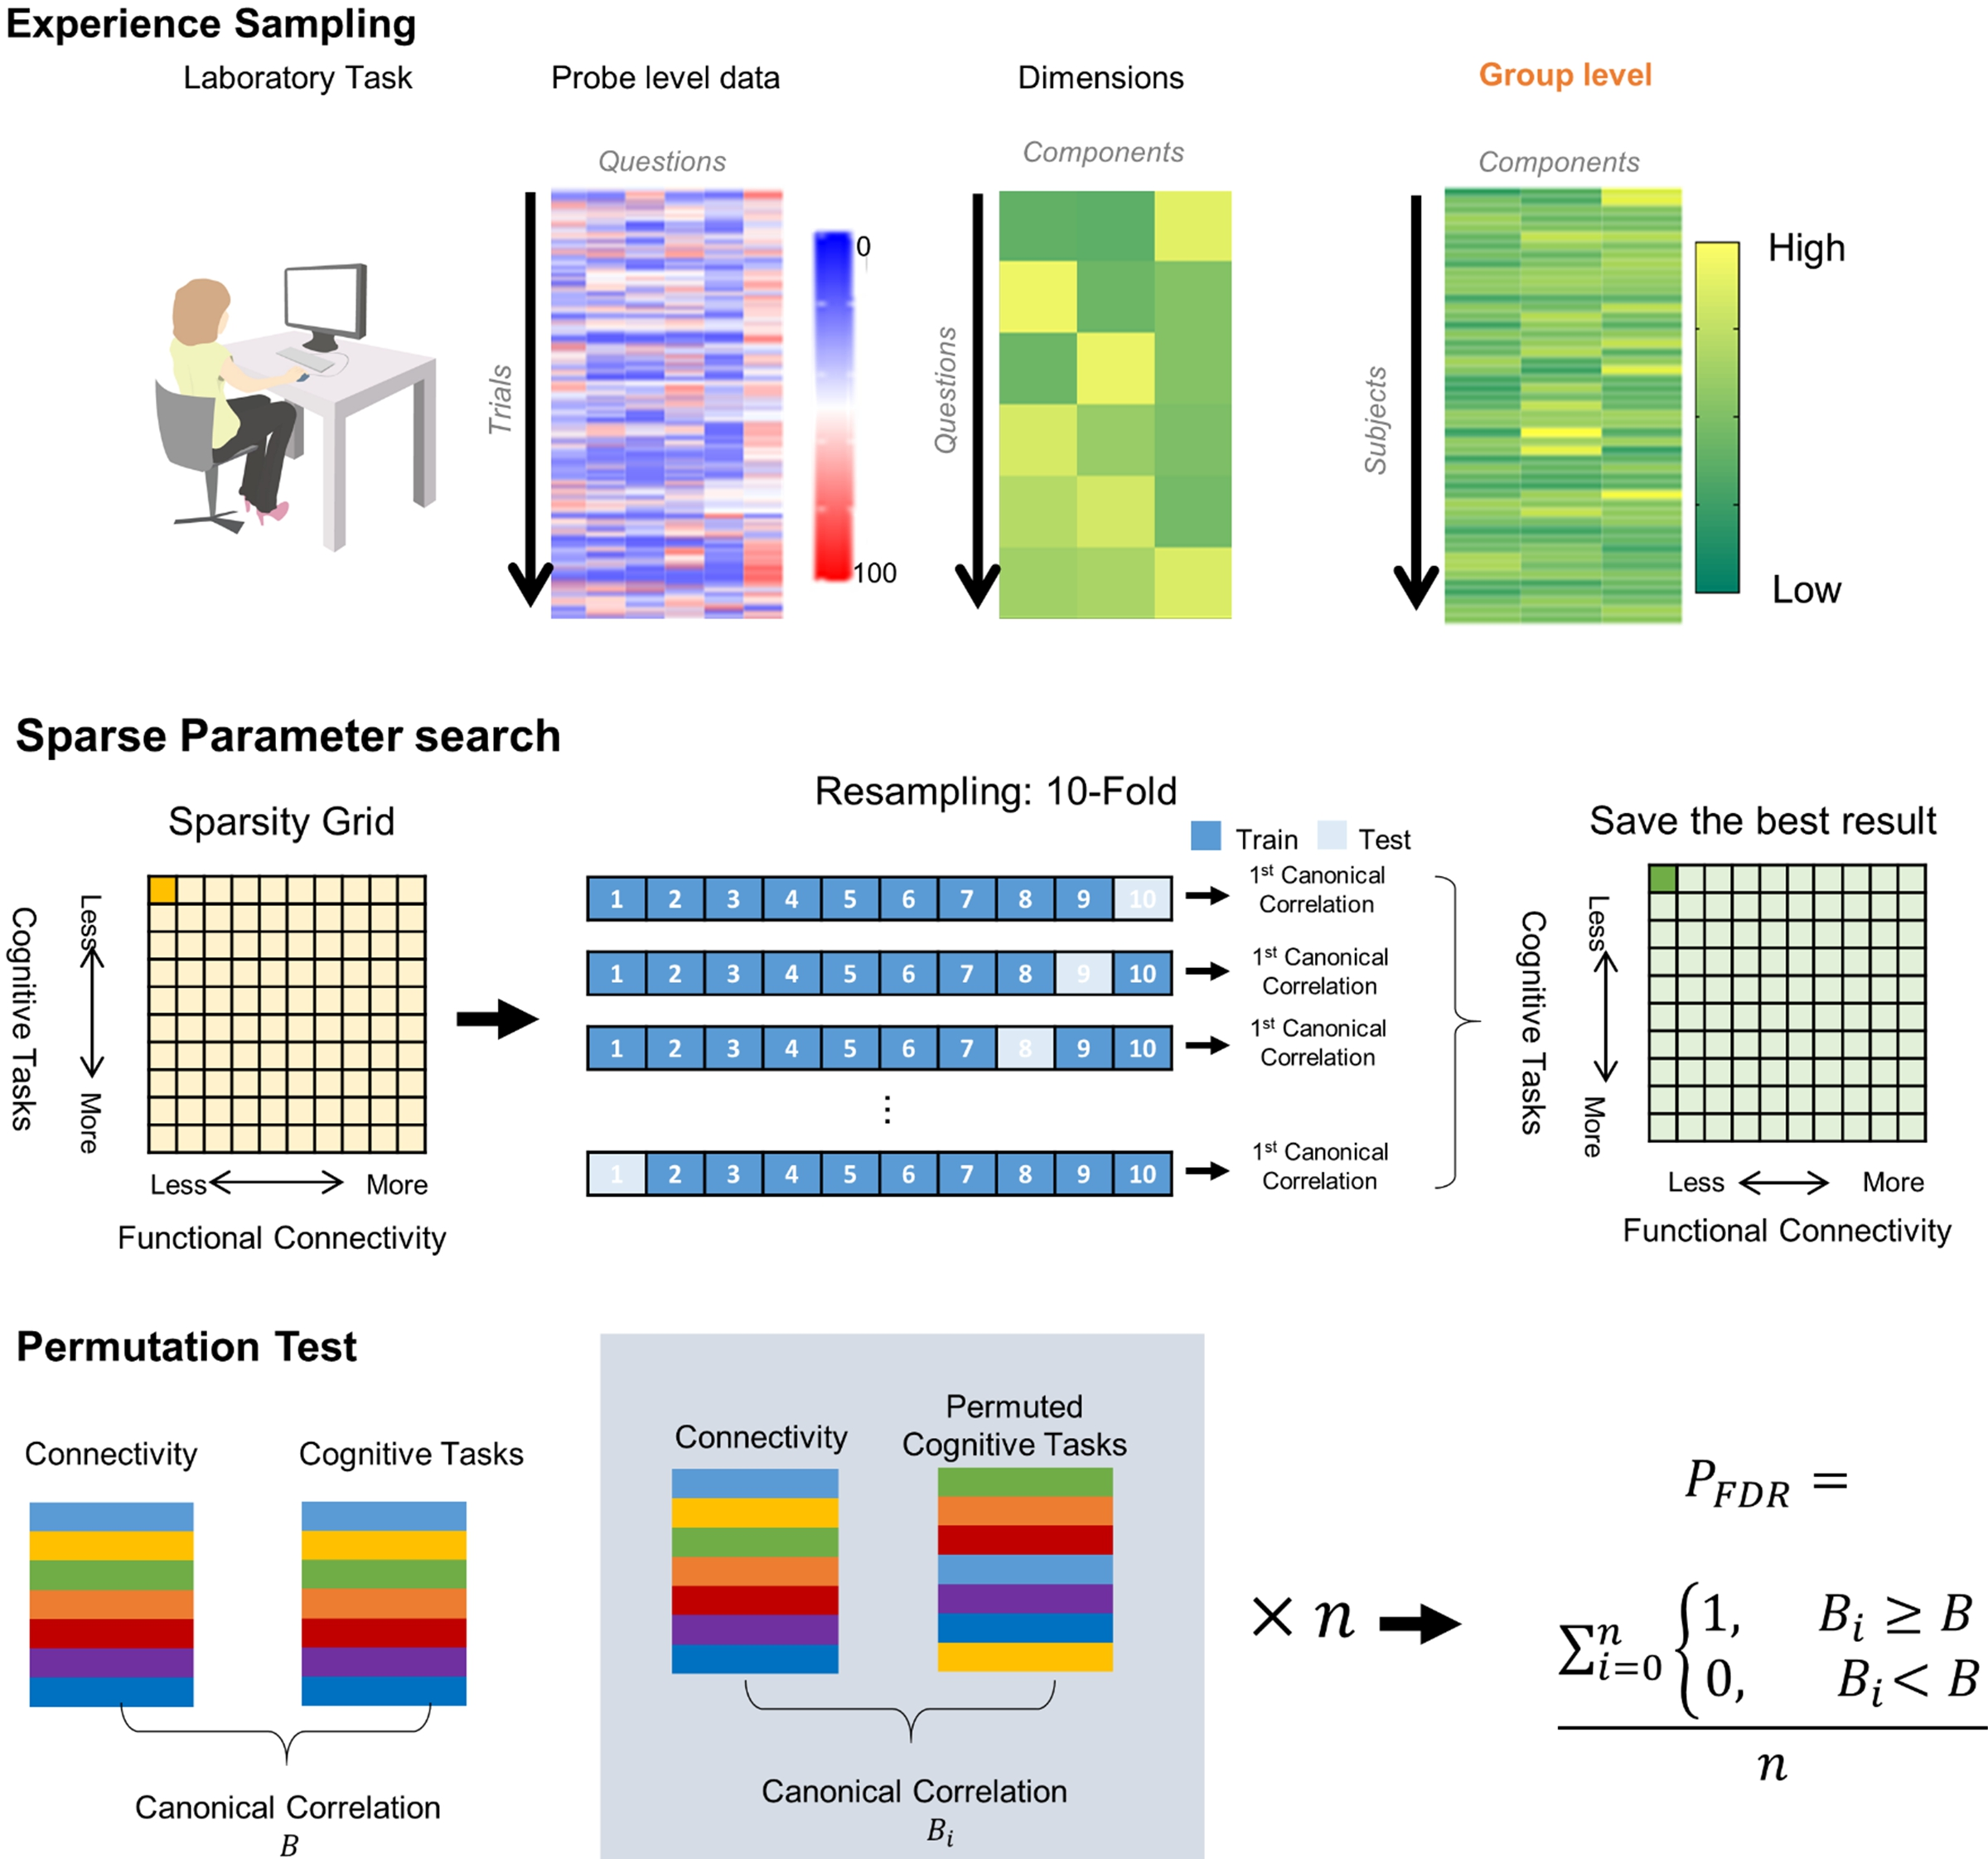
\includegraphics[width=1\textwidth]{study3/image/study3fig1.jpg}
    \caption{Analysis pipeline.}
    \label{fig:study3:fig1}
    \caption*{\footnotesize{
    Top: PCA on MDES (\cref{study3:method:e:mdes}).
    Middle: sparsity parameter selection (\cref{study3:method:f:1}). 
    Bottom: permutation test procedure (\cref{study3:method:f:1}).
    }} % eleborate
\end{figure}

\subsection{Group analysis}
\label{study3:method:g}

To determine how patterns of unconstrained neurocognitive activity related to performance on the self-report experience summarised in three different ways (see section \ref{study3:method:e:mdes}),
we conducted three independent statistical analysis on the identical subjects. A Type III multivariate multiple regression with Pillai's trace test was applied to the data. Each of the latent components describing the neurocognitive mechanism from the SCCA was the independent variables, and the 13 measures from MDES were the dependent variables. We hoped to described the neurocognitive components by the linear combination of the self-report questions collected via MDES. The p-values reported were based on Bonferroni correction. The analysis was conducted in R (version 3.3.1). The multivariate multiple regression was conducted in R (version 3.3.1) using function \texttt{Manova} in R package \texttt{car} (companion to applied regression, version 2.1–5).

% ==========================================================================================================
\section{Results}
\label{study3:results}

\begin{wrapfigure}{o}{0.5\textwidth}

    \centering
    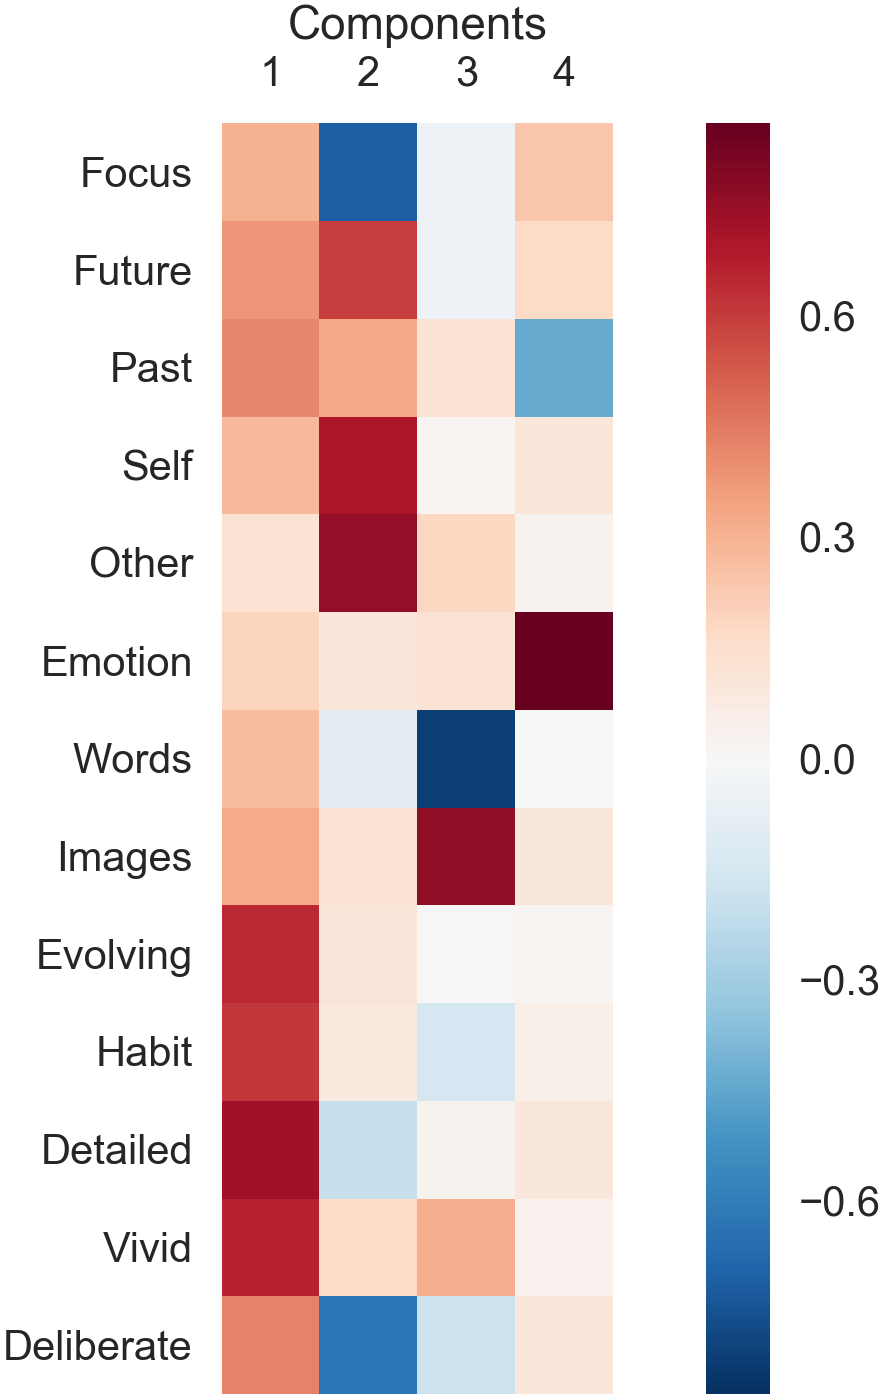
\includegraphics[width=0.48\textwidth]{study3/image/study3pca.png}
    \caption{Dimensions of ongoing though.}
    \caption*{The result from the PCA is presented as a heatmap. The colour bar represents the value of the principal component loading.}
    \label{fig:study3:figPCA}

\end{wrapfigure}

\subsection{Dimensions of ongoing thought}
Experience sampling probes revealed four unique dimensions of ongoing thought during the 0-back/1-back task. PCA of the 13 experience sampling questions resulted in four principle components of thought presented in \cref{fig:study3:figPCA}. Consistent with our prior study \cite{Poerio2017}, the components were characterised as: detailed thought, off-task thought, modality of thought, and emotional thought.


\subsection{Neurocognitive component selection}

Sparse Canonical Correlation Analysis (SCCA) was used to determine connectome-wide dimensions that describe common variance shared by descriptions of brain and experience. This took as input individual scores for the connections between each of the regions extracted from Yeo's 7 networks parcellation and the 13 cognitive task scores.

\begin{wrapfigure}{o}{0.5\textwidth}
    \centering
    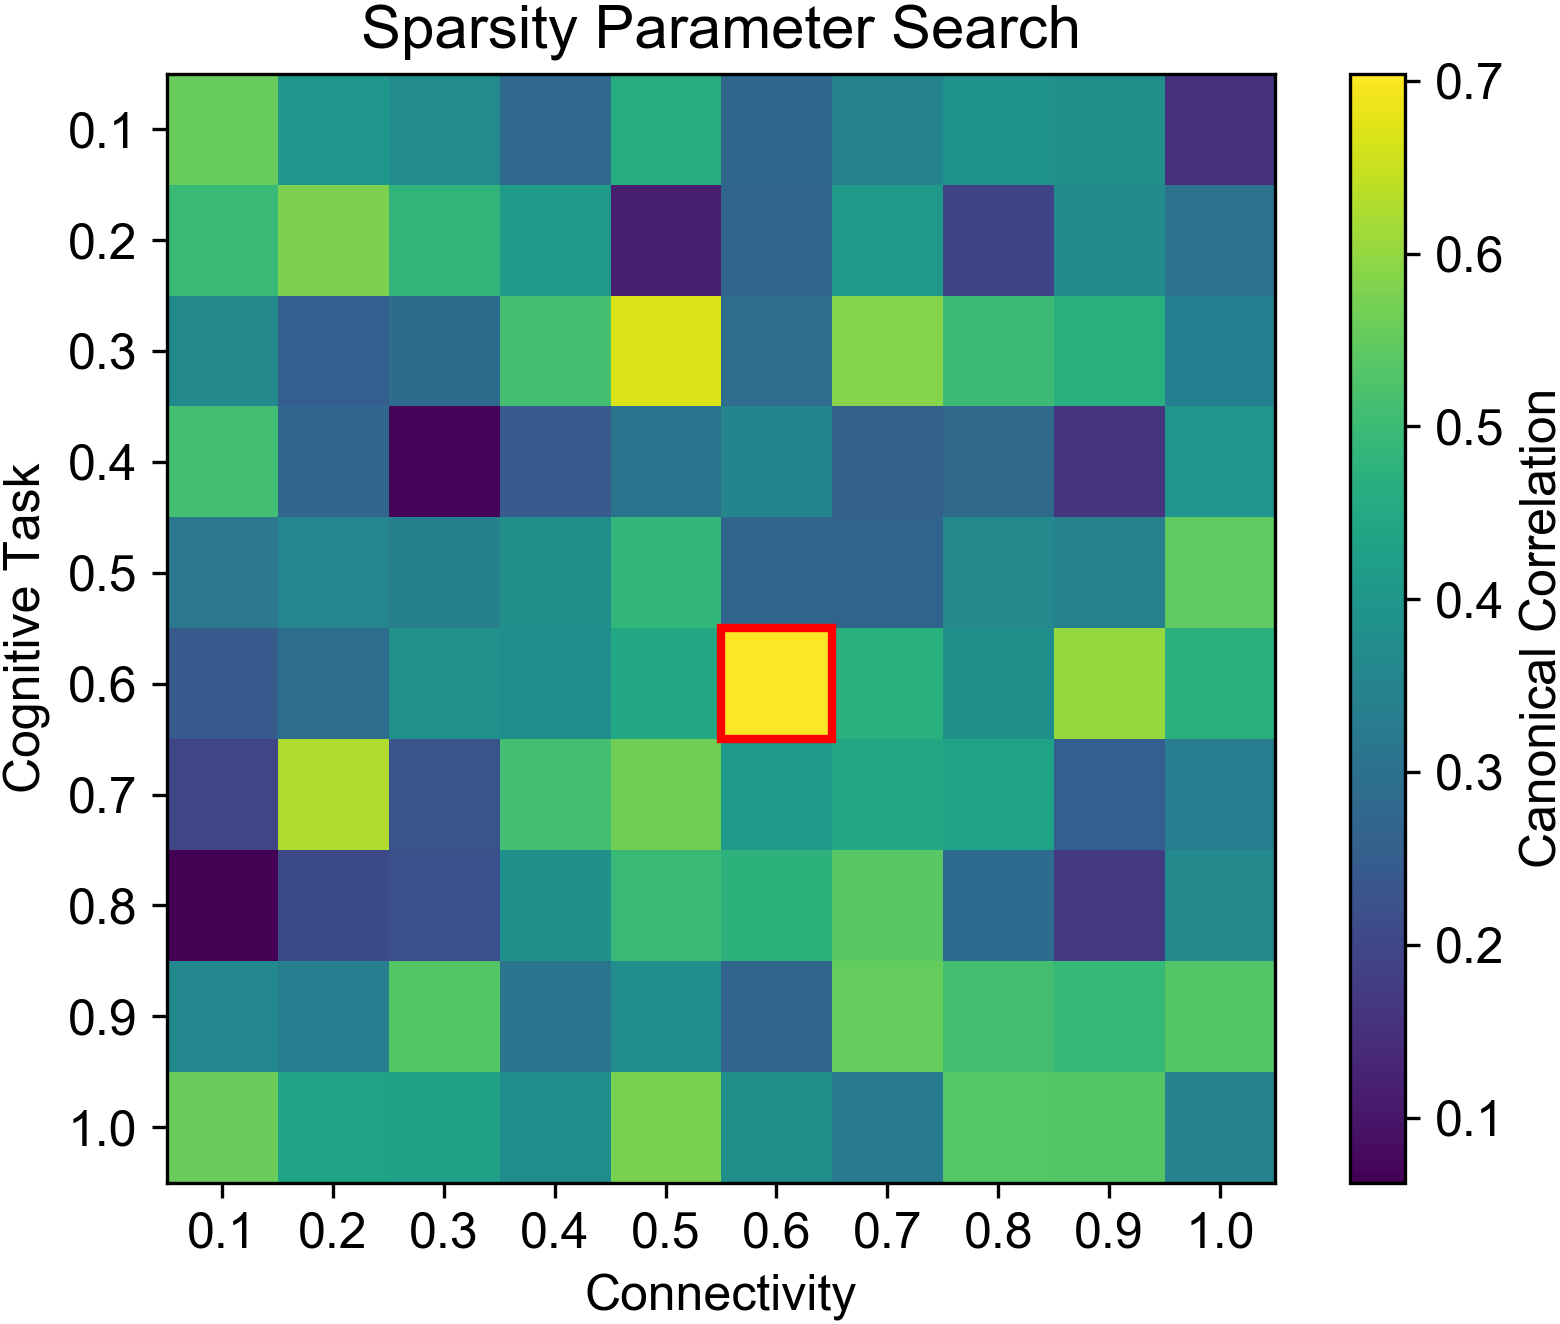
\includegraphics[width=0.48\textwidth]{study3/image/study3fig2.png}
    \caption{Grid search result.}
    \caption*{This heatmap represents the rank-1 canonical correlations of each sparsity coefficient pairs determined by the CV. The red square indicates the best result.}
    \label{fig:study3:fig2}
\end{wrapfigure}

We applied SCCA with 10-fold CV and permutation tests as the model selection strategy. We obtained penalty levels of 0.6 on both the functional connectivity and cognitive tasks indicated the best out-of-sample prediction on our data through the grid search (Figure \ref{fig:study3:fig2}), obtaining 0.70 on the rank-1 canonical correlation. Five significant canonical components were identified through FWE-corrected p-value through permutation tests. The p-values of the 5 components are 0.028, 0.042, 0.041, 0.012, 0.033. The canonical correlations of the 5 significant latent components were 0.68, 0.68, 0.68, 0.70, and 0.68. Since the sparsity turns CCA into a convex optimisation problem, the modes didn't come out in the descending order of their canonical correlations.

\subsection{Determining constituent category of cognitive functions}
\label{study3:results:category}

The latent components yielded by the best model are presented in \cref{fig:study3:fig3}. Using SCCA we identified five neurocognitive dimensions characterised at the cognitive level as the creative association (Component 1), fluid intelligence (Component 9), temporally specified cognition (Component 7), and, separate dimensions of episodic memory linked to visual (Component 8) and verbal (Component 12) codes of representation. For the ease of presentation and interpretation, we summarised the components as network-network connectivity instead of 57-by-57 connectivity matrices. The heat maps describe the network-to-network correlations and the cognitive tasks.

\begin{figure}[H]
    \centering
    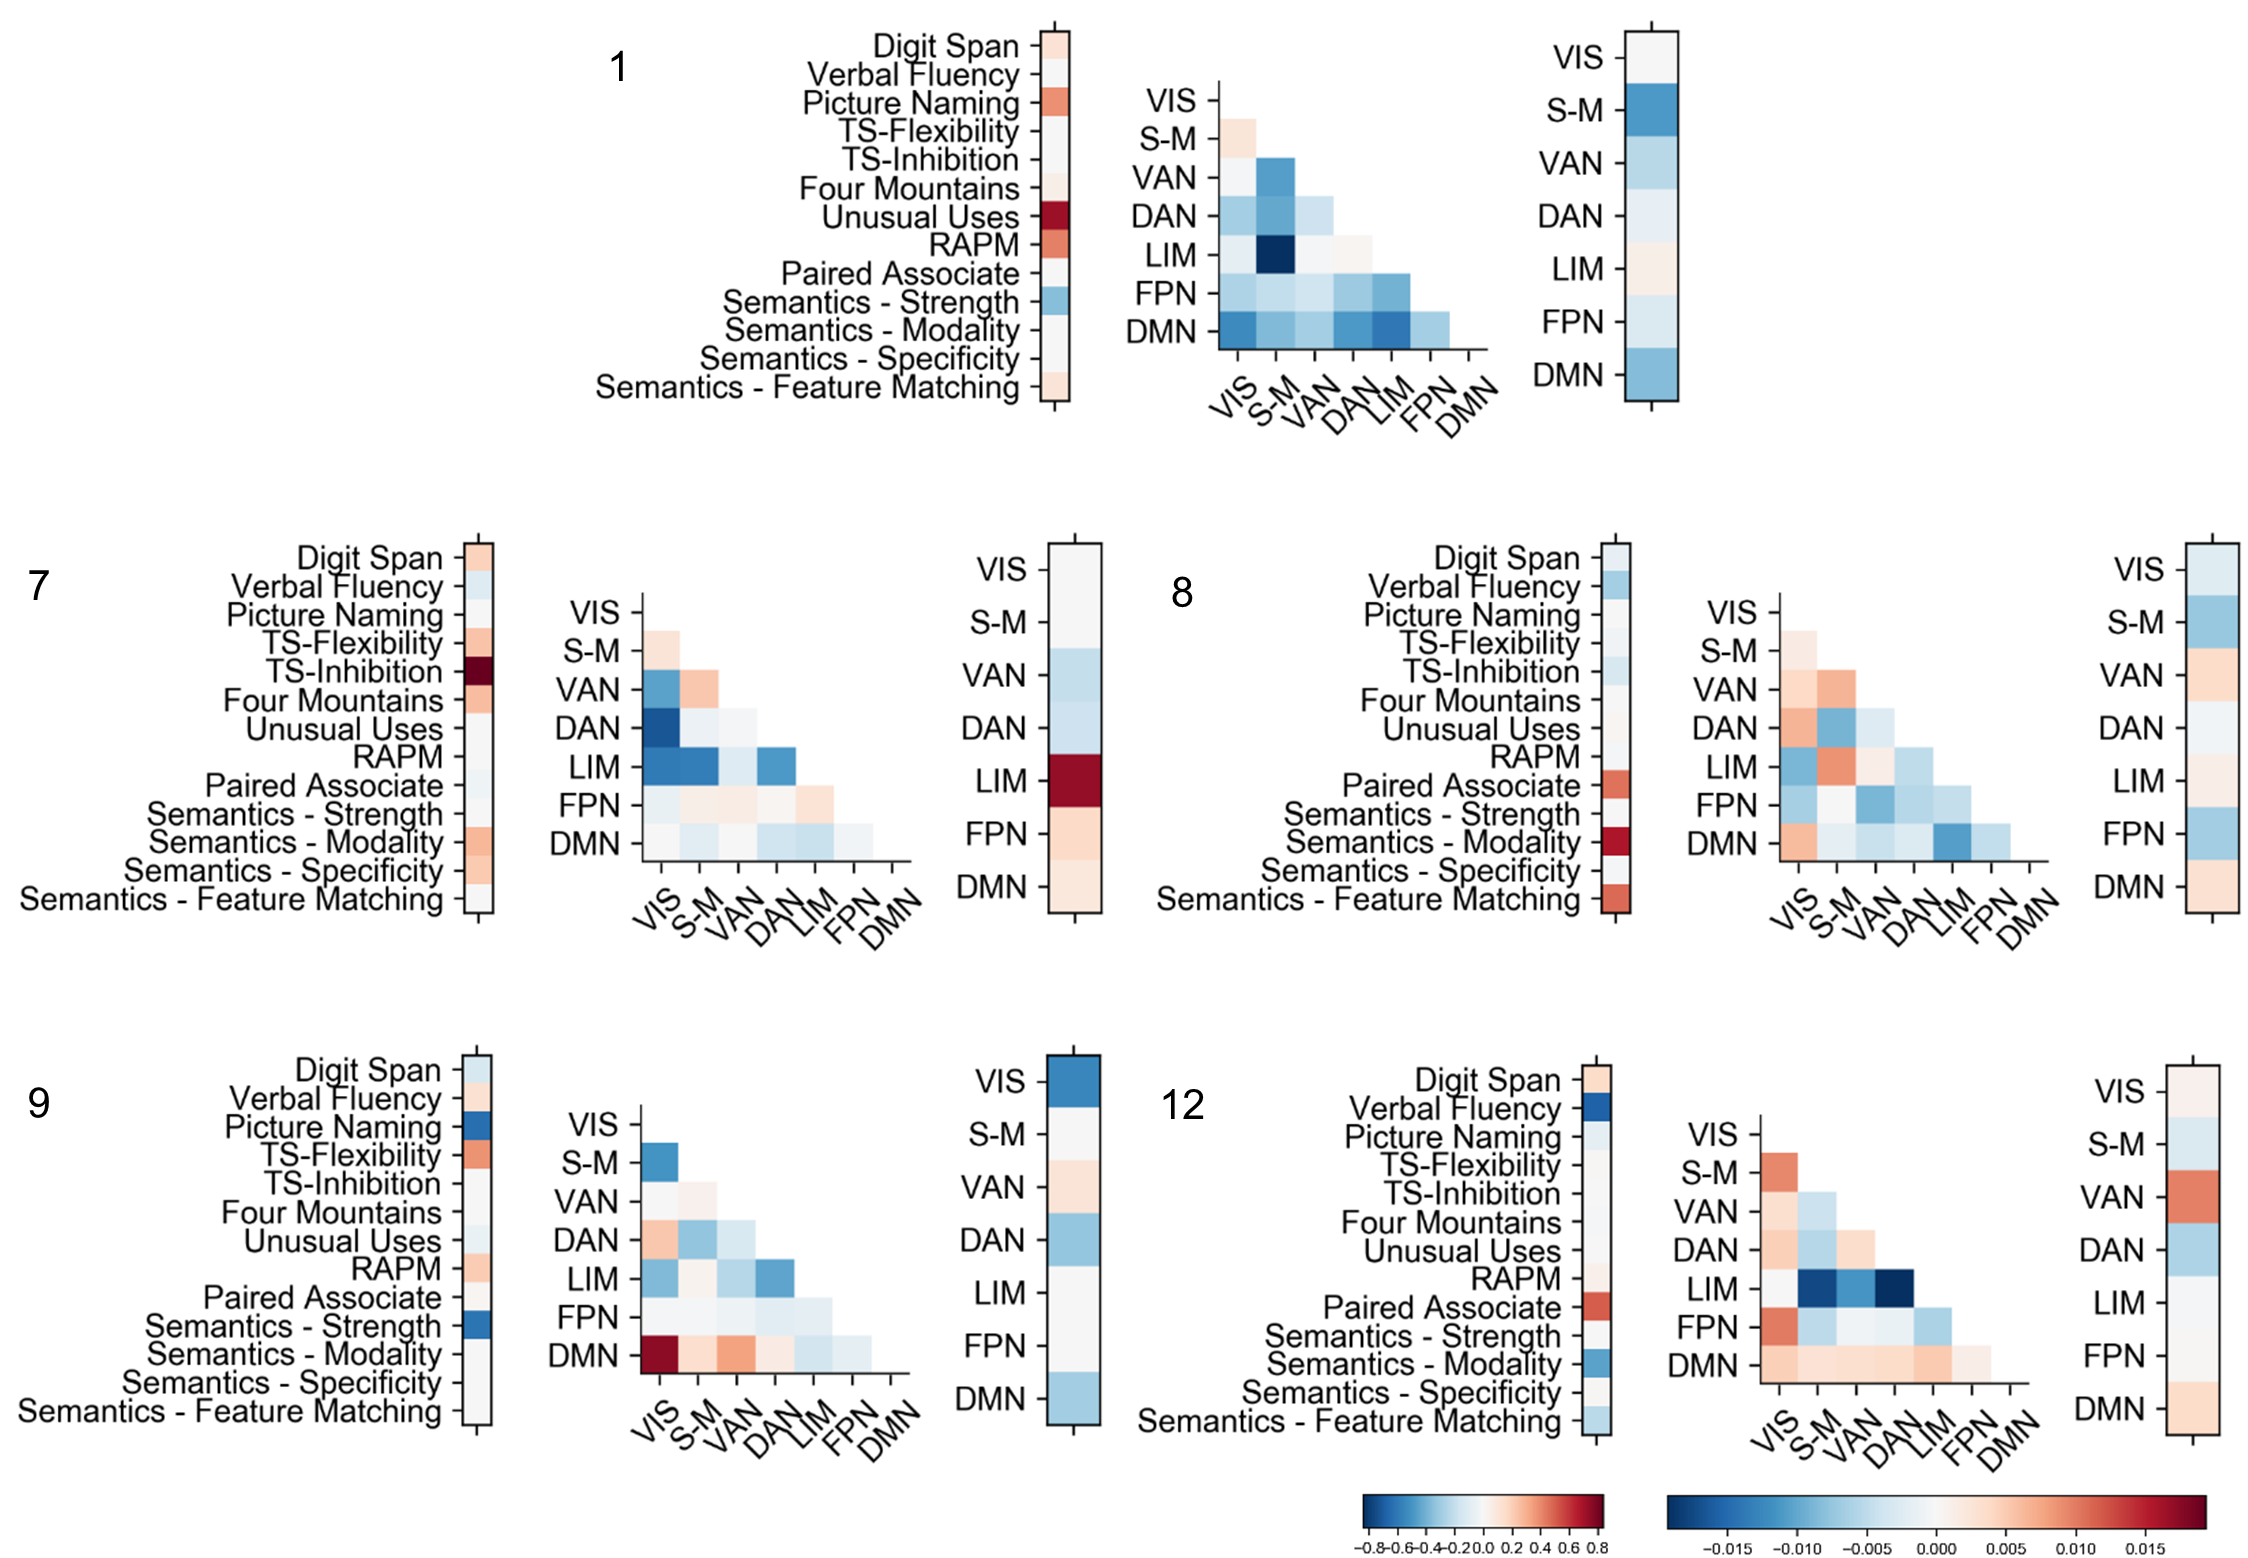
\includegraphics[width=1\textwidth]{study3/image/study3fig3.png}
    \caption{Significant components from SCCA.}
    \caption*{The colour in the heatmap indicates the value of the canonical coefficients of each components. VIS: visual network, S-M: somatomotor network, VAN: ventral attention network, DAN: dorsal attention network, LIM: limbic network, FPN: frontoparietal network, DMN: default mode network.}
    \label{fig:study3:fig3}
\end{figure}

% explain the significant components
Component 1 emphasis semantic control with the picture-naming task and the unusual uses task, along with intelligence in the cognition component. The negative coefficient in semantic strength indicated the ability to detect weaker semantics relationships. The functional connectivity pattern shows a general dissociation among all networks, except between the unimodal systems. Network segregation was especially pronounced between the sensorimotor network and the limbic system, and a general dissociation between the unimodal sensory system and the attention and transmodal regions. Component 1 demonstrated semantic control ability to generate mental representation and semantic associations. 

Component 7 reflects better performance on task switching tasks, both in terms of a reduced switch cost, and the ability to suppress prior mental sets. The performance was better for both visual semantic decisions and specific semantic imagery. In addition, participants performed better on the four mountains task and had a larger digit span. This pattern of performance was linked to the better performance of tasks that requires mental representations to be controlled across time (task switching, four mountains task and digit span) particularly with a particular emphasis on visual processing. The connectivity pattern shows strong connectivity between sensory systems. In addition, the visual system showed reduced connectivity between the attention systems, while the limbic system was less correlated with all systems other than the FPN. Within network connectivity was strong for the limbic, frontoparietal and default mode networks. Overall, this component demonstrates the ability to control representations over time and is linked to integrity within limbic and transmodal systems and separation between visual and attention systems.

Component 8 pits executive tasks against verbal episodic memory systems since it is linked to better paired-associate memory, verbal semantic memory and feature matching and worse task switching, digit span and verbal fluency. The functional connectivity pattern shows a general pattern of reduced network connectivity.  Exceptions to this include the unimodal networks – the visual network shows stronger connections to attention and default mode networks, while the sensorimotor network shows stronger coupling to the ventral attention and limbic networks. Within network connectivity is higher in the ventral attention, limbic and default mode networks. 

Component 9 is composed of tasks that rely on controlled processing (fluid intelligence, task switching, fluency and controlled semantic retrieval). It is also linked to worse picture naming. In connectivity terms, the default mode network shows stronger connectivity with unimodal and attention networks, and the dorsal attention network is linked to stronger connectivity with the visual network. Within network connectivity is low within the visual, dorsal attention and default mode networks and high in the ventral attention network. 

Component 12 highlights the between episodic memory (better paired-associate memory) and worse visual semantic memory (worse verbal semantics and poor figure matching). Fluency was better when organised alphabetically rather than by categories. The default mode network and the visual system showed a general coupling pattern with the other networks, while a strong dissociation of the limbic with the attention systems and the sensorimotor system. The component demonstrates a strong ability to retain and recall information that does not benefit from the semantic organisation.

\subsection{The relationship between neurocognitive components and self-reports on thoughts}
\label{study3:results:group}
% multivariate main effect

Three regression models were performed to evaluate the relationship between neurocognitive components and self-reports on thoughts: average scores of all thought probes thought probes in 0-back and 1-back conditions (\cref{fig:study3:fig4}). 

We first examined the relations of the neurocognitive components and the overall thought reports. In the model of all thought probes, we got multivariate main effect in component 7 (\textit{F}(13, 160) = 2.239, \textit{p} = .010, \paretasquared = .154)
and 12 (\textit{F}(13, 160) = 1.946, \textit{p} = .029, \paretasquared = .137). There was only one significant univeriate effect after Bonferroni correction, which is the negative correlation on self-question under component 7 
(\textit{b} = −0.25, 95\% CI = [−0.40, −0.10], \textit{t}(172) = -3.369, \textit{p} = .005). The results revealed two types of thought patterns. Component 7 focuses on information maintenance in cognitive tasks and the integration within the separated transmodal systems. The related thought patterns shows a low tendency in reporting personal issues. Although there were no significant contributing univariate pattern in component 12, we see a trend of deliberate, focused thought pattern with low imagery information related to retrieval of semantically novel associations.

Two models examined the average scores of thought probes during the 0-back and 1-back condition separately.  The aim is to uncover potential differences in thought reports under the two conditions. In the 0-back condition, only component 7
(\textit{F}(13, 160) = 1.924, \textit{p} = .031, \paretasquared = .135)
showed the main effect in multivaraite level. There was only one significant univeriate effect after Bonferroni correction, which is the self-question under the model for component 7 
(\textit{b} = −0.23, 95\% CI = [−0.37, −0.79], \textit{t}(172) = -3.03, \textit{p} = .017).
In the 0-back condition, the participants perform a visual matching task. The focused state during the 0-back condition is associated with more cognitive mechanism that sustains ongoing thought. 

The 1-back condition model showed significant results in
component 7
(\textit{F}(13, 160) = 2.192, \textit{p} = .012, \paretasquared = .151)
and component 12
(\textit{F}(13, 160) = 2.312, \textit{p} = .008, \paretasquared = .158). There was only significant univeriate effect in the model for component 7 after Bonferroni correction.
The significant variable is the self question
(\textit{b} = −0.26, 95\% CI = [−0.40, −0.11], \textit{t}(172) = -3.51, \textit{p} = .003)
and the habit question
(\textit{b} = −0.22, 95\% CI = [−0.37, −0.75], \textit{t}(172) = -2.97, \textit{p} = .020).
The 1-back condition required participants to maintain meaningless associations of the two shapes presented on the screen.

\begin{figure}[H]
    \centering
    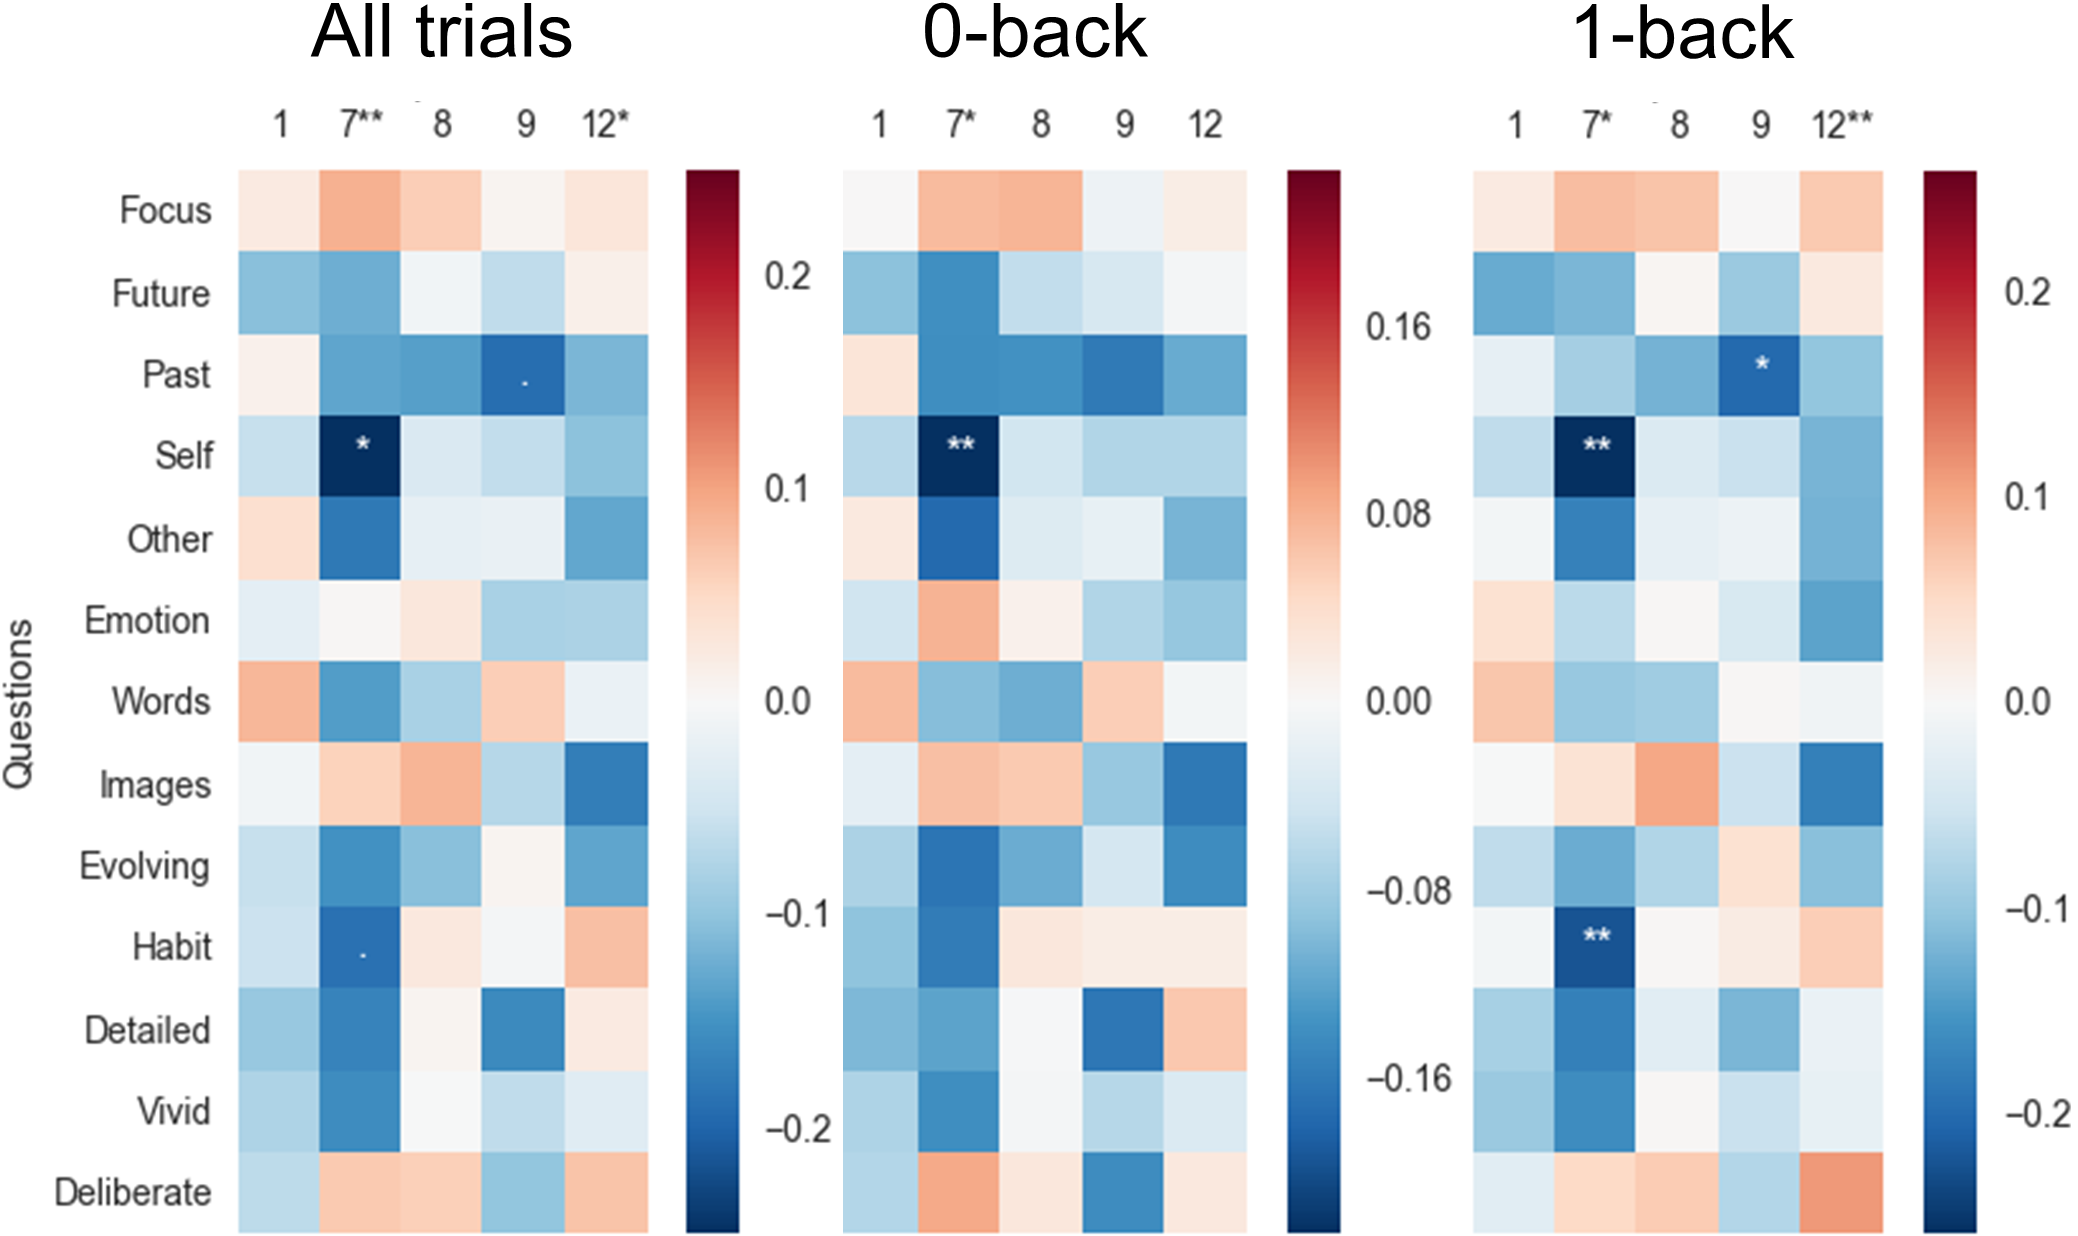
\includegraphics[width=0.9\textwidth]{study3/image/study3fig4.png}
    \caption{Group level analysis on neurocognitive components and  self-report on thoughts.}
    \caption*{
    \footnotesize{The codes next to the component number indicate the significant level of the mutivariate results, and those in the coloured cells are for the univariate results. The colour represent the univariate \textit{b} value. P-value significant codes: `***': \(<0.001\);  `**': \; `*': \(<0.05\); `.': \(<0.01\)}
    }
    \label{fig:study3:fig4}
\end{figure}


\subsection{The relationship between neurocognitive components and ongoing thought patterns}

Pearson's correlations were calculated to explore the relationships between the neurocognitive components and the dimensions of ongoing thought. The temporally specific cognition component (Component 7) is negatively correlated to details and off-task components (\cref{fig:study3:figcorr}). 


\begin{figure}[H]
    \centering
    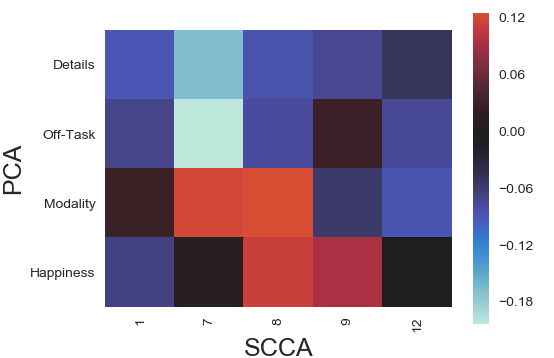
\includegraphics[width=0.6\textwidth]{study3/image/pca_cca_corr.png}
    \caption{The relationships between the neurocognitive components and the ongoing thought.}
    \caption*{This heatmap represents correlation between the principal components and the univariate level predictions in \cref{study3:results:group}.}
    \label{fig:study3:figcorr}
\end{figure}

% ==========================================================================================================
\section{Discussion}
\label{study3:discussion}

We set out to identify patterns that described the association between different aspects of cognition and the intrinsic organisation of the cortex and to explore whether these accounted for variations in patterns of ongoing thought. Using SCCA we identified five neurocognitive dimensions characterised at the cognitive level as the creative association (Component 1), fluid intelligence (Component 9), temporally specified cognition (Component 7), and, separate dimensions of episodic memory linked to visual (Component 8) and verbal (Component 12) codes of representation. In our subsequent analysis, we identified that variation in temporally specified cognition was associated with substantial variance in patterns of ongoing thought recorded in the laboratory. In particular, we found that this neurocognitive dimension was associated with variation in both the task relatedness of cognition and its level of immersive details. In the discussion, we consider the implications of these data for theoretical accounts of ongoing thought.

In neural terms, our CCA analysis suggests that the relative degree of integration/segregation of the limbic system is at the core of whether an individuals experience is a pristine reflection of their current external goal, or instead, they are immersed in thoughts generated through imagination. We found that individuals who maintained attention on the task in hand, tended to show a pattern of brain activity dominated by whether the limbic system was coupled to itself, but decoupled from other cortical areas, while individuals who reported off-task experiences with immersive qualities showed the reverse pattern (low within network coupling, and high between network coupling for the limbic system). These data add to a growing body of evidence that highlights limbic regions as critical for patterns of spontaneous thought. For example, lesions to the hippocampus are associated with reductions in off-task thinking \cite{McCormick2018} and episodic future thinking as part of a task \cite{Maguire2011,Race2011}. Likewise, semantic dementia, which targets the lateral and medial aspects of the temporal pole, reduced the capacity to imagine the future \cite{Irish2012,Viard2014}. Furthermore, hippocampus activity has been shown to be important for spontaneous thought during the occurrence of spontaneous thought \cite{Ellamil2016}, while its connectivity with regions of the default mode network is important for both episodic features of spontaneous experience \cite{Karapanagiotidis2017} as well as its immersive features \cite{Smallwood2016}. Based on our results, the contribution of limbic structures to spontaneous experience may depend on their coupling with other regions, allowing these hub regions to integrate information from across the cortex to create a mental scene \cite{Hassabis2009}. This account is broadly consistent with views of limbic structures, such as the hippocampus \cite{Moscovitch2016} and the anterior temporal lobe \cite{Lambon-Ralph2017} which are both thought to share a hub and spoke architecture in which their contribution to cognition arise from their capacity to integrate information from across the cortical mantle.

In our analysis, participants with whom the limbic system was relatively isolated within the cortical mantle, performed well in a task switching context that required them to suppress representations of a previous task set. Prior uses of this task paradigm have documented that this ability is linked to the tendency to ruminate. \citeA{Whitmer2007} found that individuals who were high on trait rumination were better than non-ruminators when switching back to a prior task. This pattern is broadly consistent with our data which shows that people who show the smallest cost from inhibiting a prior mental set, were more likely to reports patterns of ongoing thought that were characterised by immersive experiences characterised by self-relevant, social and episodic content. Building on our study a promising area for future study would be to examine how limbic connectivity supports the recurrence of negative self-relevant experiences that are thought to be important in rumination \cite{Kleckner2017,Peters2016,Cooney2010}. 

Our data suggest that the default mode network shows a similar, albeit less pronounced pattern, to the limbic system. Given evidence of a role for the DMN in both immersive experiences in task states \cite{Sormaz2018,Richter2016} as well as in off-task states \cite{MasonScience2007,Christoff2009,StawarczykPlos2011}. It is possible that these two networks work in tandem when cognition is focused on self-relevant information with the limbic systems providing the episodic and conceptual content, and the default mode network allowing this content to be represented at a relatively abstract level. This interpretation is consistent with the observation that the default mode network is spatially located at the top of a hierarchy and most distant from unimodal inputs, while limbic regions occupy an intermediate position \cite{Margulies2016}. 

Finally, it is worth considering a number of limitations of this study. First, we did not measure patterns of ongoing thought while individuals performed the battery of cognitive tasks. It is, therefore, possible that part of the shared variance that our analyses capture emerges because of the patterns of ongoing thought occur during the cognitive tasks \cite<see>[for evidence of a similar point in the context of executive control or intelligence tasks]{MrazekJoEP2012}. However, this interpretation of our data is unlikely since individuals who were off-task tended to perform better on the tasks when they returned to a mental set that had recently been active. Second, our neural data was only measured on a single occasion, raising the possibility that this measure of brain function reflects a state rather than a trait. While this remains a possibility, recent studies have shown that individual patterns of functional connectivity remain relatively consistent across tasks and time \cite{Gratton2018}. Nonetheless, future studies could benefit from measuring an individuals architecture across multiple points to provide a more robust indication of its trait like features.


\chapter{General discussion}
\chaptermark{Discussion}
\label{ch:discussion}
%\setcounter{equation}{0}
% ==========================================================================================================
Contemporary research on patterns of self-generated thought, such as those occurring during states of mind-wandering, is riddled with contradictions. For example, the content of ongoing thought varies from future-orientated planning thoughts that may help refine personal goals \cite{Medea2016} to negative past concerns that can maintain unpleasant affective states \cite{Killingsworth2010}. Likewise, research has highlighted the disadvantage of off-task thought during tasks that demand continuous external attention \cite{McVayJOEP2009,McVay2012}, whereas research on creativity and problem solving suggests evidence of beneficial influence from off-task thought\cite{Smeekens2016,Baird2012}.

The conflict presented above is thought to emerge because of variability in the nature of ongoing thought. Heterogeneous ongoing thought may be composed of a set of experiences with overlapping features---the so-called family resemblance account of mind-wandering \cite{Smallwood2013, Seli2018}. One aim of this thesis was to develop an empirical approach sensitive to possible similarities among the heterogeneous patterns of thought. 
In particular, the goal was to identify multiple patterns of ongoing experience that share common and distinct features that can be empirically measured. To implement this goal, this thesis examined the intersection between subjective reports and objective measures---in this case patterns in resting-state functional connectivity and performance on cognitive tests. The current thesis employed SCCA \cite{WittenSCCA2009}---a multivariate approach that measures similarities of linear patterns in two domains of data. SCCA identifies various patterns of thought while reflecting the covariance between both brain and cognition.
The overarching aim of the thesis is to provide evidence in support of the family resemblance view of on-going thought that would facilitate more constrained theoretical accounts of how different patterns of ongoing thought emerge.

% ====================================================================================================================
\section{Empirical findings}
\label{ch:discussion:results}

The current thesis comprised three studies focusing on resolving the heterogeneous features of ongoing thought by considering its intersection with measures of neural function---in this case the intrinsic functional connectivity at rest. 
\cref{ch:study1} revealed that mind-wandering is a collection of different ongoing thoughts that are derived from the connectivity patterns in DMN. % study 1
\cref{ch:study2} found that the population variance in intelligence is related to different whole-brain neural hierarchies and ongoing thoughts. % study 2
\cref{ch:study3} showed that either momentary or longer mental representation is associated with the ability to inhibit prior mental sets and the balance of segregation and integration between the limbic system and the rest of the cortex. % study 3
This section of this thesis describes in detail two themes that emerged from this work---the heterogeneity of patterns of ongoing thought and the integration and segregation of transmodal networks.

\subsection{Heterogeneity}

In the mind-wandering literature, converging evidence highlights heterogeneity in the variety of functional outcome linked to off-task thought \cite{SmallwoodFrontiers2013}, the definitions that researchers have used to study different types of ongoing thought \cite{SeliTiCS2016}, and the number of competing theoretical accounts \cite<e.g.>{Smallwood2010,McVay2010}. The current thesis aimed to systematically explore whether this conflicted literature is a consequence of the emergence of distinct patterns of ongoing thought with different experiential features and associated outcomes. This question was explored by focusing on a single candidate neural system---the DMN (\cref{ch:study1}) and at the whole-brain level (\cref{ch:study2}).

It is a widely held view that the DMN is important in certain types of ongoing thought \cite<see a review from>{SmallwoodSchooler2015}. The aim of \cref{ch:study1} was to explore whether associations between patterns of DMN connectivity and measures of experience yielded unique patterns with distinctive patterns of functional outcomes. In this study, we found two reliable neuroexperiential patterns each with distinct functional outcomes (see \cref{fig:study1:fig4}). Internal connectivity in mPFC related to positive habitual experience was predicted by poor executive control (see \cref{fig:study1:fig2}), suggesting that this may correspond to patterns of executive failure linked to the mind-wandering state \cite{McVay2009}. The relationship between ongoing thought deficits in executive control could be a result of failure to allocate cognitive resource to the external task. In addition, patterns of PCC-TPJ-mPFC decoupling (see \cref{fig:study1:fig2}), associated with off-task experience, provided a link to better performance on tasks requiring the generation of information.  The continuous content generation associated with an external task is similar to the association between patterns of off-task thought and creativity \cite{Baird2012}. Together, \cref{ch:study1} provided evidence that ongoing thoughts unfold along a set of heterogeneous dimensions. Critically, \cref{ch:study1} explained how the conflicts between the representational and executive failure accounts could be a consequence of different configurations in the DMN.

Since the brain works as a distributed system when engaging in tasks, a natural question following \cref{ch:study1} is how regions other than DMN contribute to the heterogeneity of ongoing thought. Recent works on the hierarchical functional cortical organisation suggest variability in relationships among large-scale networks \cite<e.g.>{Margulies2016}. In \cref{ch:study2}, the focus shifted from the DMN to the whole brain in order to explore the contribution of other brain networks to the heterogeneity of ongoing experience. The identified neuroexperiential components suggested that different patterns of ongoing thought may be linked to distinctive neural hierarchies. For example, experiences characterised as purposeful monologue (see component 1 in \cref{fig:study2:fig2}) were linked to sensory segregation---dissociation between the DMN and unimodal networks---at the whole-brain level. This pattern of decoupling is a well-documented element of ongoing thought \cite<see>{Smallwood2013,SmallwoodFrontiers2013} and is thought to reduce the interference between patterns of self-generated thought and events in the external environment \cite{Murphy2018}. Consistent with the adaptive view on the sensory segregation process, this patterns of experience was linked to better performance on measures of cognition and intelligence (\cref{fig:study2:fig3}). The study also highlighted that dysfunctions within a second hierarchy---the MDN \cite{Duncan2010}---may also make an important contribution to patterns of ongoing thought (see component 3 in \cref{fig:study2:fig2}). Individuals whose thoughts were directed towards their personal concerns had low levels of connectivity within both the ventral and dorsal attention networks, as well as the FPN. Critically, these individuals tended to show poor performance at measures of intelligence and control. This phenotypical pattern provide evidence for the hallmarks of executive failure \cite<i.e.>{McVay2010}. In contrast to data present in \cref{ch:study1}, where a singular system gives rise to different patterns of thoughts and behaviour, the data presented in \cref{ch:study2} shows that heterogeneous patterns of ongoing thought emerge from functional connectivity that reflects previously documented neurocognitive associations.

Multiple overlapping patterns of ongoing thought can be realised by combining experiential data with objective neurocognitive measures. The demonstrations in the current thesis suggest that some of the theoretical controversies relates to ongoing thought can be explained as relating to distinct patterns of ongoing thought. For example, in both \cref{ch:study1,ch:study2}, we found certain patterns of ongoing experience that have beneficial features (such as better creativity or intelligence) and others with less beneficial correlates (such as lower intelligence or worse executive control). Based on these findings, some of the controversies regarding whether mind-wandering should be considered a failure of executive control \cite<e.g.>{McVay2010,Smallwood2010} result from prior studies lumping together of experiential states with different features into a single category. In other words, one important contribution of this thesis is providing a synthesis to resolve the competing theoretical positions of the same phenomenon. The competing elements highlighted in the theoretical accounts can be seen to reflect independent aspects of ongoing thought. The capacity to identify these overlapping patterns of experience is made possible in part because of the use of a biological marker (i.e. functional connectivity) as well as assessments on multiple aspects of ongoing thought and task performance. Moving forward, studies of ongoing thought would, therefore, benefit from measuring multiple dimensions of experience, as well as measures of covert function such as neuroimaging measures, pupillometry \cite{Konishi2017}, or other biological measures \cite{Engert2014}. 


\subsection{Integration and segregation in transmodal networks}

A second theme emerging from this thesis lies in the transmodal networks. Patterns of heterogeneity emerge through differential patterns of integration and segregation between and within large-scale neural systems. Integration and segregation have been both assumed to be an important principle in brain organisation. 
%DMN
For example, hierarchical integration of sensory information is thought to support more abstract aspects of cognition \cite{Mesulam1998}. In contrast, segregating neural systems are thought to provide flexibility in the operations that can be performed \cite{Buckner2013}. A hierarchical organisation implicating both integration and segregation is captured by the primary gradient which stretches from the unimodal to the transmodal networks \cite{Margulies2016}.
%MDN
Other examples of cognitive hierarchies that depend on integration and segregation include the MDN \cite{Duncan2010}. The integrated activity of large-scale network concerned with integration and segregation is important whenever individuals perform complex goal-directed tasks.  Notably, the principal gradient and the MDN are differentiable in terms of the degree of separation between the DMN and FPN. The differences in functional distance indicate how patterns of integration within transmodal cortex is a defining feature of the neurocognitive hierarchies. 
%limbic 
The other hierarchy emerges from the limbic system. This limbic system hierarchy is composed of visceromotor regions that connect with DMN, and salience network \cite{Kleckner2017}. These authors suggest that this forms an allostatic-interoceptive system, segregated from the unimodal and attention systems. This hierarchy is assumed to emerge because the limbic system can selectively integrate information from systems involved in attention and cognition, as well as those important for emotion and affect. 
%short summary on past study
These past studies illustrate that at the core of different neural hierarchies are patterns of integration and segregation between distributed neural regions.

This thesis underscores the implication of the importance of integration and segregation in the neural hierarchies that support patterns of ongoing thought. \cref{ch:study1} demonstrated that the role of the DMN in distinct patterns of ongoing thought emerges because of differences in the integration and segregation within DMN, with spontaneous off-task thought linked to lower connectivity within this system, while the positive habitual thought was linked to integration within the same system. Importantly, this latter pattern of experience was also linked to stronger coupling with a number of regions outside of the DMN including left temporoparietal cortex, left hippocampus/entorhinal cortex, left lateral middle temporal gyrus, and the left pre-SMA. We also found evidence for integration and segregation in \cref{ch:study2}. The pattern of purposeful future planning thought was linked to segregation between DMN and the primary sensory systems. The second pattern of thoughts reflected ongoing thoughts of personal importance and was linked to reduced connectivity (i.e. lower integration) within many regions of attention and control systems. Within both \cref{ch:study1,ch:study2} patterns of ongoing thought were differentiable based on the patterns of integration and segregation between neural systems.

The most powerful evidence for integration and segregation within this thesis is provided by \cref{ch:study3}. This analysis highlighted the integration and segregation in the limbic system as a core determinant of patterns of ongoing thought. The limbic system has been previously argued to form a hierarchy integrating the transmodal system while simultaneously segregating the unimodal system to facilitate attention inhibition \cite{Kleckner2017}. In Study we found a pattern of population variation anchored at one end by a highly inter-connected limbic system, integrating with the other transmodal area and segregated from the sensorimotor system. Such segregation pattern was predictive of behaviour that entailed the flexibility of retaining mental content. At the other extreme, the limbic system was highly coupled with neural system and individuals were unable to inhibit their prior mental set. Importantly, we found that this pattern of population variation was linked to patterns of ongoing thought that varied from task-focused thought at one end to personal, habitual content at the other. This analysis not only suggests that the degree of integration and segregation between the limbic system is important for attentional control \cite<i.e.>{Kleckner2017}. Moreover, it also suggests that the degree to which this system is coupled or decoupled from other aspects of the cortex is a primary determinant of whether patterns of ongoing thought are focused on the task, or are instead focused on personally relevant matters in a detailed manner.

Together the three studies presented in this thesis show that at the core of different patterns of ongoing thought are the integration and segregation between neural systems. Moving forward studies should formally consider how patterns of integration and segregation between neural systems can give rise to the heterogeneity of patterns of ongoing thought that make up our daily lives.


\section{Limitations}

% trait vs state
The primary limitation of this work is how it dealt with the temporal elements of cognition. For example, the studies focused exclusively on individual differences within a population rather than a state level of ongoing thought. Studies exploring the associations between static functional connectivity and psychological traits have brought fruitful results to ongoing thought \cite{Smallwood2016,McVay2009,RubyPlos2013}. However, it is import to bear in mind that these studies confound traits with states since a defining feature of patterns of ongoing thought is their intermittent nature. While individual traits allow a way to understand links between cognition and the brain, it remains to be seen whether the patterns discovered at the population level will be applicable in the momentary state. 

There are two ways that future studies could provide a more valid temporal perspective on patterns of ongoing thought. One approach would be to measure experience and neural activity on multiple occasions. One potential strategy is collecting multiple examples of experience using online probes while the neural function is recorded. Recently using the same 0-back/1-back task in conjunction with measures of neural function provided by fMRI we found that different dimensions of experience can have unique neural representations \cite{Sormaz2018}. It would be possible to apply CCA to data collected in this manner which would allow neurocognitive patterns to emerge that describe momentary states rather than population variation. A second approach would be to explore the association between patterns of dynamic neural function and ongoing experience. The recent discovery of temporal dynamic using hidden Markov models \cite<HMM;>{Vidaurre2017} demonstrated that time spent in brain states predicts behavioural traits including measures of inhibition control and attention. HMM allow the identification of temporally re-occurring states that are defined by a similarity between neural data across time. It is possible that the application of HMM to neural data would resolve covert patterns of neural function that reflect momentary changes in patterns of ongoing thought.

Another limitation emerges from the statistical technique that was applied in this thesis in terms of both model selection strategy employed. The three studies in the current thesis explored and improved the model selection strategy of SCCA. The analysis in \cref{ch:study1} did not select the hyper-parameters in a data-driven manner. With formal hyper-parameter selection, \cref{ch:study2} is more transparent and data-driven in the model selection. A nested cross-validation scheme was adopted to simultaneously select the hyper-parameter and the final model. With the motivation to construct a pipeline that can be generalised to the basic version of linear CCA, \cref{ch:study3} separates the hyper-parameter selection step and the mode selection. The final canonical correlations of the principle mode improved from 0.28 in \cref{ch:study2} to 0.70 in \cref{ch:study3} with a simpler pipeline. The scope of the current thesis focuses on the psychological question of ongoing thought, hence the two pipelines presented in \cref{ch:study2,ch:study3} are not formally bench-marked on the same data set. Future work a structurally simple and well-performed pipeline would be important for the application of CCA and its variation on biomedical data.

The other concern is the choice of optimisation target for model selection. The current thesis uses out-of-sample explained variance as the learning target. The rationale is to maximise the potential of predictability in a wider unknown sample with the limited sample size. The alternative choice would be the out-of-sample prediction error, which minimises the mistake when applied to an unknown sample. This thesis did not explore the second option, hence the performance is unknown. These two optimisation targets are asking two fundamentally different questions---explained variance provides a more optimistic view of the model, while prediction error is more conservative. It is uncertain whether the choice of learning target should be question-driven or performance-driven. Again, a bench-marking study would be helpful to clarify the potential of the options. 



\section{Future directions}

Before concluding it is worth considering the implications for two specific areas of the study of ongoing thought. Much debate has been around the intermittent disruption caused by experience sampling methods when intending to measure the train of thought in a concurrent task \cite{SmallwoodSchooler2006}. This problem is especially concerning with MDES, where participants spend around a minute to report the thought rather than one or two questions that can be done in seconds. A covert marker would allow studying the ongoing thought while not interrupting the natural flow of thought.

This thesis shows that the variation in whole-brain functional hierarchy potentially supports different types of ongoing thought. If, as this thesis suggests, patterns of integration and segregation in neural activity are important aspects of different features of ongoing thought, then the covert marker could be based on patterns of functional connectivity. However, the calculation of connectivity depends on the processing of time-series data making the determination of rapid temporal changes problematic. This is compounded by the low temporal resolutions of fMRI. The application of magnetoencephalography (MEG) is possibly helpful for the determination of online marker, given its ability to reveal neural processes at the level of milliseconds superior to fMRI.

In conclusion, the current thesis provided a proof of principle on the utility of whole-brain functional connectivity in exploring ongoing thought. It has the potential to be the covert online marker for spontaneous thought. However, with the current limitation in fMRI temporal resolution, functional connectivity calculation would be the main challenge of such application. MEG is the possible candidate method for understanding the dynamic of ongoing thought and underlying neural pattern.


% ==========================================================================================================

\section{Concluding remarks}
\label{ch:discussion:summary}

This thesis set out to examine the neurocognitive mechanism of ongoing thought and establish the basic component processes to incorporate the heterogeneity of ongoing thought. Three major questions were posed at the start of the thesis. These will now be revisited in light of the work performed.

\textbf{Why does ongoing thought show both costs and benefits?} Ongoing thought is a collective phenomenon with multiple types of experience each with their own associated functional outcomes at the trait level. This thesis suggests that pattern of costs and benefits related to mind-wandering may be usefully conceptualised as characterising overlapping but distinct aspects of the ongoing experience. Further work will be important to understand the underlying mechanisms that explain why these different states emerge.

\textbf{Can functional neural hierarchy explain the heterogeneity?} This thesis demonstrates that ongoing thoughts with different experimental profiles are associated with different neural hierarchy. Further work is suggested to incorporate the neural basis with the ongoing thought profiles at the state level to understand the dynamic of ongoing thought.

\textbf{Is the family resemblance view viable for ongoing thought?} Overall this thesis supports the contention that ongoing thought can be conceived of as a family of experiences with similar and overlapping features. The current thesis finds common component processes that determine population variation. Further work is necessary on the application of these findings at a state level to improve the understanding of the architecture of the component processes.

% appendices
% latex does not allow nested imports, so include all appendices in this file as a separate 'chapter'

\appendix
\setcounter{chapter}{0}

\renewcommand{\chaptername}{Appendix}
\renewcommand{\theequation}{\Alph{chapter}.\arabic{section}.\arabic{equation}}
\setcounter{equation}{0}
\addcontentsline{toc}{chapter}{\numberline{}Appendix}

% ==========================================================================================================

\chapter{Chapter \ref{ch:study1} Supplemental Materials}
\label{appendix:study1}
\textit{Adapted from the online supplemental material of: }\\
Wang, H.-T., Poerio, G. L., Murphy, C. E., Bzdok, D., Jefferies, E., \& Smallwood, J. (2018). Dimensions of Experience: Exploring the Ontology of the Wandering Mind. \textit{Psychological Science}, 29 (1), 56–-71. doi: 10.1177/0956797617728727
% ==========================================================================================================
\section{Questionnaires}
\label{appendix:study1:subsection1}

\subsection{Health Organization Adult ADHD Self-Report Scale}
This is a self-report screening scale of adult ADHD, developed by the world health organisation\cite{Kessler2005}. This questionnaire comprises 18 questions to access the frequency of DSM-IV Criterion A symptoms of adult ADHD. We take the average scores across all 18 questions to access the participants’ ADHD tendency.

\subsection{Autism Spectrum Quotient}
The Autism Spectrum Quotient \cite{Baron-Cohen2001} comprises 50 questions, included 10 questions measuring 5 different dimensions: social skills, attention switching, attention to detail, communication, and imagination. For each questions the participant has four options: definitely agree, slightly agree, definitely disagree, and slightly disagree. ‘Definitely agree’ or ‘slightly agree’ responses scored 1 point on half of the designated questions.  ‘Definitely disagree’ or ‘slightly disagree’ responses scored 1 point on the other half of the questions.  The scores of each dimension is calculated with the sum of the scores of designated the questions.

\subsection{British Dyslexia Association Dyslexia checklist}
The British Dyslexia Association Dyslexia checklist \cite{Smythe2001} comprises 15 questions to access the tendency of dyslexic. Each answer of the questions have a designated scores. Individuals scoring less than 45 are probably non-dyslexic; individual scoring 45 – 60 shows a mild level of dyslexia; scoring above 60 suggests moderate or severe dyslexia. The score in the current study is the sum of the scores.

\subsection{World Health Organization Quality of Life}
The World Health Organization Quality of Life \cite{WHOQOL2002} assessment measures the quality of life cross-culturally.  In the current study, a shorter version of the original instrument, WHOQOL-BREF, was used, as it is recommended for large research studies. WHOQOL-BREF comprises 26 questions. The assessment measure the following broad domains: physical health, psychological health, social relationships, and environment. The official scoring system can be obtained on request from the official website.

\subsection{CES-Depression scale}
The CES-Depression scale \cite{Radloff1977} is a self-report scale designed to measure the symptoms of depression in the general population. The scale contains 20 questions accessing the frequency of depressive symptoms in the past one week. In the current study we used the sum of the scores as an indicator of depression.

\subsection{State-Trait Anxiety Inventory}
The State-Trait Anxiety Inventory \cite{Spielberger1987} is a measure of trait and state anxiety, composing with 20 state anxiety questions and 20 trait anxiety questions. The state anxiety questions measure the level of anxiety when taking the questionnaire; the trait anxiety questions measure the general level of anxiety. The questions are rated on a 4-point scale. Mean scores of the state and trait questions were taken as our measurement, where higher scores indicates a greater level of anxiety.

\subsection{Ruminative Response Scale}
The Ruminative Response Scale \cite{Treynor2003} is a 22-question self-report measure of rumination. Rumination involves introverted focus on negative mood and was found associating with depressive symptoms and stress \cite{Moberly2008a}. The questions are rated on a 4-point scale. Mean scores of the questions were taken as our measurement, where higher scores indicates a greater level of rumination.

% ==========================================================================================================
\section{Cognitive tasks}
\label{appendix:study1:subsection2}
The behavioural tasks were allocated into three sessions based on apparatus needed. Visual attention and generative semantic tasks were in session A, and semantic and episodic memory tasks were in session B and C. In each session, the first and second tasks were the mind-wandering task and the flanker task. In session B and C, the third task was the encoding and the delayed-recall phases of the word pair memory task respectively. The rest of the tasks were performed based on a pre-allocated order.
\subsection{General apparatus of the laboratory session}
In session B and C, the participants were in a sound proofed booth with a big glass window for the testers to monitor them. There were four testing spaces separated by office screen dividers. The tasks were delivered on Windows 7 computers and presented on 21 inches LCD monitors. Headsets were given to participants to deliver audio stimulus and blocking distracting noises. Participants were instructed to view the screen from a distance of 65 cm. The participants raised their hand to inform the experimenter to start each task. In session A, the visual attention tasks were delivered on a Windows 7 computer and presented on a 21 inches CRT monitor in a small room with light switch. The generative semantic tasks were delivered on a Windows 7 computer and presented on a 21 inches LCD monitor and a headset with microphone attached were used to recording verbal responses.
\subsection{Semantic tasks}
The tasks employed a 3 alternative force choice (3AFC) paradigm with the probe presented alongside the three choices among which the target was selected. There are four tasks: Relatedness Task (Word-to-Picture Matching; Word-to-Word Matching; Picture-to-Picture Matching), Identity Matching Task(Word-to-Picture Matching), Feature Matching Task, and Scrambled Picture Matching as the control task.

The unrelated distracters of each trial were selected among the targets from other trials ensuring that they were not linked to the probe. Except for the Feature Matching Task, all the tasks contain the same trial structure. Each trial started with 500ms blank screen. The three choices were subsequently presented on the bottom of the screen for 900ms. Finally the probe was presented on the top middle section of the screen. Probe and choices remained visible until participants’ response or for a maximum of 3 seconds. In the Feature Matching Task, the 500ms blank screen was replaced by the probe with, in bracket, the feature (cue) as criterion for the matching (colour, size, shape or texture). Probe and cue were presented for 1000ms. The three choices were subsequently presented on the bottom of the screen. Probe, cue and choices were presented as written words and remained visible until participants’ response or for a maximum of 3 seconds.

The stimuli employed in the tasks were selected from a larger dataset of words and photographs used in previous experiment
\cite{Davey2015, Krieger-Redwood2012, Krieger-Redwood2015, Whitney2012}.
The pictures were coloured photographs collected on internet and re-sized to fit the trial structure (200pixel, 72 dpi). All the coloured pictures and words were rated for familiarity and imageability using 7-point Likert scales. Lexical frequency count for the words was obtained by the SUBTLEX-UK database \cite{VanHeuven2014}.

For the details of the design, please refer to the online supplementary material of \cite{WangPsychScience2018}.

\subsection{Fluency Task}
During Verbal Fluency \cite{Adlam2010,Balota2008}, participants had 1 minute to generate as many unique words as possible belonging to a semantic category (category fluency) or starting with a specific letter (letter fluency). Semantic fluency was assessed for six categories split in two blocks (Block A: fruits, vehicles, type of dogs; Block B: animals, tools, type of boats). Letter fluency was assessed for three letter cues (Block C: A, F, S). Block order was counterbalanced across participants and the order of cues within each block was randomized. Participants’ verbal responses were collected and the audio recordings were transcribed and scored off-line.

\subsection{Word pair memory task}
Participants also undertook a Word Pair Memory Task (WPMT) to assess episodic memory \cite{Cairney2016}. 80 words were selected from an adapted version of The University of South Florida (USF) word association, rhyme, and word fragment norms \cite{Nelson2004} to create 40 semantically unrelated cue and target word pairs (e.g. owl – frame). Both the cue and target words were singular and they were matched for concreteness (t(39) = 0.39; p = .696), lexical frequency (t(39) = -4.71; p =.640), word length (t(39) = 0.09; p =.933) and number of syllables (t(39) = -0.73; p = .472). There were no pre-existing forward or backward associated relationships between any of the words, reducing the likelihood of erroneous associations between words in separate pairs.\\
During an initial learning phase, participants were presented with the unrelated words pairs, one at a time for 5 seconds each. This encoding phase was followed by a recall phase during which they attempted to recall the second word from the first word in the pair, they had 12 seconds for each trial and received a feedback after each response. In case of no response or error the feedback included the correct match. Participants were required to reach a performance criterion of 60\% correct responses, with a maximum of three repetitions of the recall phase for the entire list of word pairs. In the subsequent behavioral testing session that took place at least one day apart, participants attempted to recall the pairs immediately (without feedback) and provided a confidence rate about each of their responses using a 7-point Likert scale.

\subsection{Digit span}
For the Forward and Backward Digit Span Test we used the stimuli and the score procedure described in the WASI battery. For each trial, audio files of each digit were played in the sequential order reported in the WASI battery. The Forward and Backward Digit Span versions were tested in separate blocks and instructions were presented at the beginning of each block asking participants to listen to the sequence of numbers and type them in the same order, for the Forward block, or in reverse order for the Backward block.

\subsection{Flanker task}
We used the flanker task paradigm developed by \cite{Eriksen1974} as a baseline executive measure in this study. This task is conducted at the beginning of each laboratory sessions. The target was an arrowhead at the centre, pointing to the left or right direction. This target was flanked on either side by two to four items. The items were arrows in the same direction (congruent condition), or in the opposite direction (incongruent condition), or lines (neutral condition). The participant’s task was to identify the direction of the centrally presented arrow by pressing the left arrow key for the left direction and the right arrow key for the right direction. The stimuli were white and displayed on a black background. Each trial lasted for 4000 msec. A trial started with a fixation period of 900 - 2100 msec and then the target and the flankers appeared simultaneously. The target and the flankers were presented until the participant responded but for no longer than 1700 msec.  After the participant made a response, the target and flankers disappeared immediately and then a post-target fixation cross was presented. The duration of the post-target fixation period was based on the duration of the first fixation and RT (4000 ms minus duration of the first fixation minus RT). After this interval, the next trial began.

\subsection{Task-switching task}
\label{appendix:study1:subsection2:TS}
We used the task-switching paradigm developed by \cite{Mayr2000} and the design and task materials were constructed based on \cite{Whitmer2007}. This task measured executive control on inhibiting previously relevant information. In this task, the participant identified the spatial location of a deviant object with a verbal instruction cue. The participant used a number pad to respond. Number 1,2,4, and 5 were used. Each of them responded to the spatial location of the designated rectangle. In each trial, four blue rectangles arranged into a two-by-two matrix were displayed on screen. The rectangles can vary from each other on one of three dimensions: size, motion, or orientation. Before a set time interval of 100ms or 900ms, a verbal cue on dimensions appeared on the centre of the screen. There were one practice block and two experiment blocks. The cue-stimuli interval in the practice is 500 msec, and 900 msec and 100 msec respectively in the two experiment blocks. The trials are categorised into four: control, inhibitory, uncategorised switch and repeat, see \cite{Whitmer2007} for details.

\subsection{Four mountains task}
We used the four mountains task developed by \cite{Hartley2007} as a measure of spatial scene construction memory. In this task, the participant identified the target image that match the topography of the sample image across 30 trials. The participant was presented with a sample image of four mountains for 10 seconds, and then a four-choice of landscapes arranged in a two-by-two grid shown on the screen. The participant had no limit on thinking time for each trial, and they pressed number 1 to 4 to select the image. The target image is the same landscape as the sample image, but the perspective and environment (lighting, weather and vegetation) is changed.

\subsection{Ravens advanced progressive matrices}
The Ravens Advanced Progressive Matrices \cite<RAPM>{Raven1998} measured ‘educative ability’ – that is the ability to make sense and meaning out of complex non-verbal stimuli. In order to complete the task participants were tasked with finding new patterns and relationships between the stimuli. The RAPM used in the current study contained two tests: (i) practice test - containing 2 problems and (ii) the full test – containing 36 problems. For each problem a set of 9 boxes (ordered in a 3x3 design) were shown on the screen. All but one box contained a pattern. At the bottom of the screen were 4 additional boxes, each containing a unique pattern. Participants were required to select out of these 4 potential boxes which pattern should go in the empty box. During the practice phase participants were given online feedback outlining whether their response was correct and, if not, how they should decide which box was the correct answer. If participants had any further questions, then they were instructed to ask the experimenter before starting the main experiment. During the full test no feedback was given. Participants were given 20 minutes to complete as many problems as they could, the problems got progressively more difficult.

\subsection{Unusual uses task}
The Unusual Uses Task \cite{Guilford1967} assessed divergent thinking and creativity. Participants were instructed to list as many unusual uses as they can for a familiar object. Three objects were selected (newspaper, brick and shoe). Uses were considered ‘unusual’ if they were not the original use of the item. For example, saying ‘crosswords’ for newspaper would not be considered unusual, however saying ‘animal bedding’ would. For each object, the object name appeared on screen for two minutes and participants were required to type as many unusual uses as they could. The total number of unique uses they listed for each item was calculated. Repetition of uses was not included (e.g., saying ‘animal bedding’ and ‘bedding for animal cage’ would only count as one unusual use).  The participant’s creativity score was based upon the mean number of unusual uses across the three objects.

% ==========================================================================================================
\newpage
\section{Supplementary analysis and figures}
\label{appendix:study1:subsection3}

\begin{table}[htbp]
\caption{Correlation between motion parameter (Mean FD Jenkinson) and variable of interests}
\resizebox{\textwidth}{!}{
  \begin{threeparttable}

     \begin{tabular}{r S S S S S S S S S S S}
        \toprule
         & \multicolumn{1}{c}{1-back} & \multicolumn{1}{c}{0-back} & \multicolumn{1}{c}{SEM} & \multicolumn{1}{c}{EXE} & \multicolumn{1}{c}{GEN} & \multicolumn{1}{c}{AD} & \multicolumn{1}{c}{SOC} & \multicolumn{1}{c}{DYSL} & \multicolumn{1}{c}{ATT} & \multicolumn{1}{c}{Positive/Habit} & \multicolumn{1}{c}{Spontaneous off task}\\
        \midrule
        \textit{r} & -0.140 & 0.161 & -0.186 & -0.234 & -0.046 & 0.002 & -0.007 & 0.043 & -0.007 & 0.057 & -0.096\\
        \textit{p} & 0.080 & 0.044 & 0.020 & 0.003 & 0.566 & 0.981 & 0.931 & 0.597 & 0.928 & 0.514 & 0.271\\
        \textit{N} & \multicolumn{1}{c}{157} & \multicolumn{1}{c}{157} & \multicolumn{1}{r}{157} & \multicolumn{1}{r}{157} & \multicolumn{1}{c}{157} & \multicolumn{1}{c}{157} & \multicolumn{1}{c}{157} & \multicolumn{1}{c}{157} & \multicolumn{1}{c}{157} & \multicolumn{1}{c}{134} & \multicolumn{1}{c}{134}\\
        \bottomrule
     \end{tabular}
    \begin{tablenotes}
      \item We selected participants for whom movement greater than .2mm occurred on less than 5\% of the resting state data (\textit{N} = 134) and re-ran the SCCA.

    \end{tablenotes}
  \end{threeparttable}
  \label{tab:S1}
}
\end{table}
% ==========================================================================================================

\begin{figure}[htbp]
	\centering
	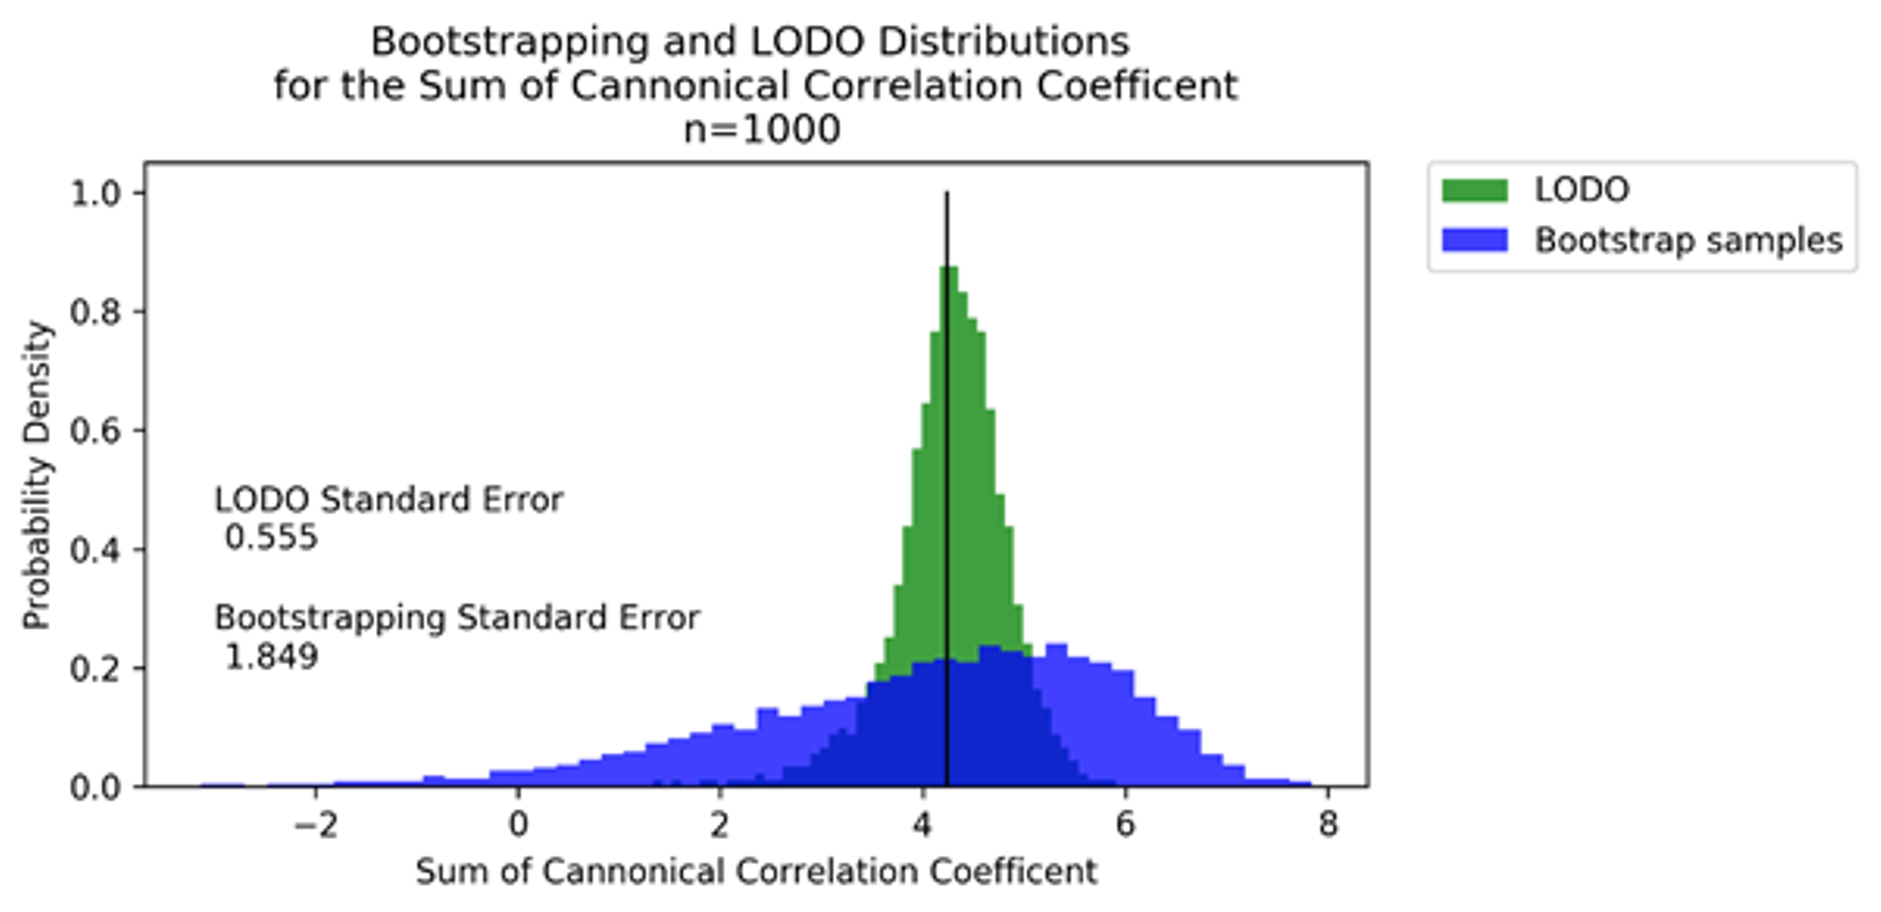
\includegraphics[width=0.8\textwidth]{append/image/study1figs1.png}
	\caption{Restricted temporal sampling and bootstrapping resampling distribution with 1000 iteration.}
	\label{fig:3S1}
\end{figure}
% ==========================================================================================================
\begin{figure}[htbp]
	\centering
	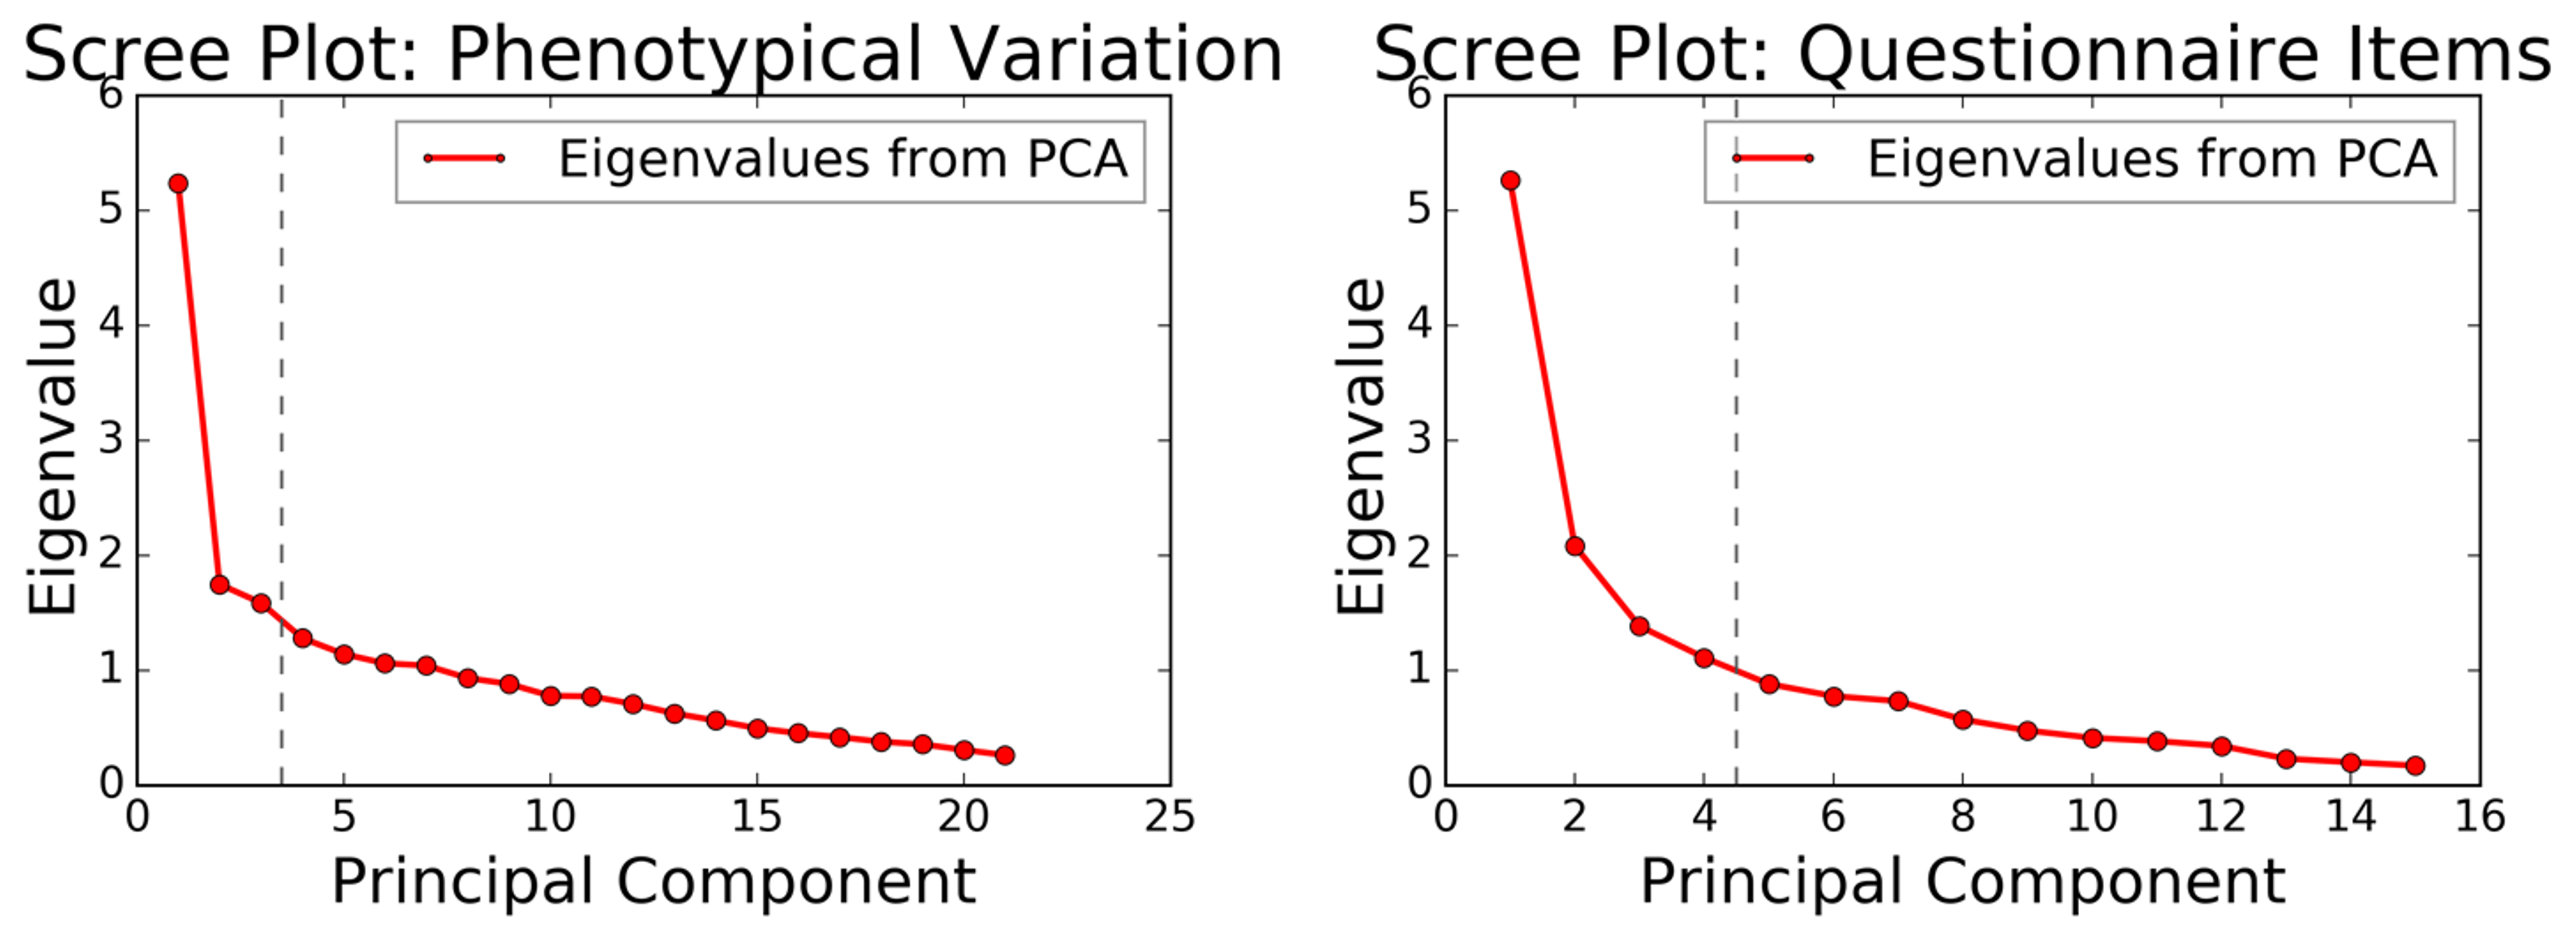
\includegraphics[width=0.8\textwidth]{append/image/study1figs2.png}
	\caption{Scree plots of the principle component analysis.}
	\label{fig:3S2}
\end{figure}
% ==========================================================================================================
\begin{figure}
    See Online Supplemental Material \url{http://journals.sagepub.com/doi/suppl/10.1177/0956797617728727}
    \caption{Full set of components.}
	\label{fig:3S3}
\end{figure}
% ==========================================================================================================
\begin{figure}
	\centering
	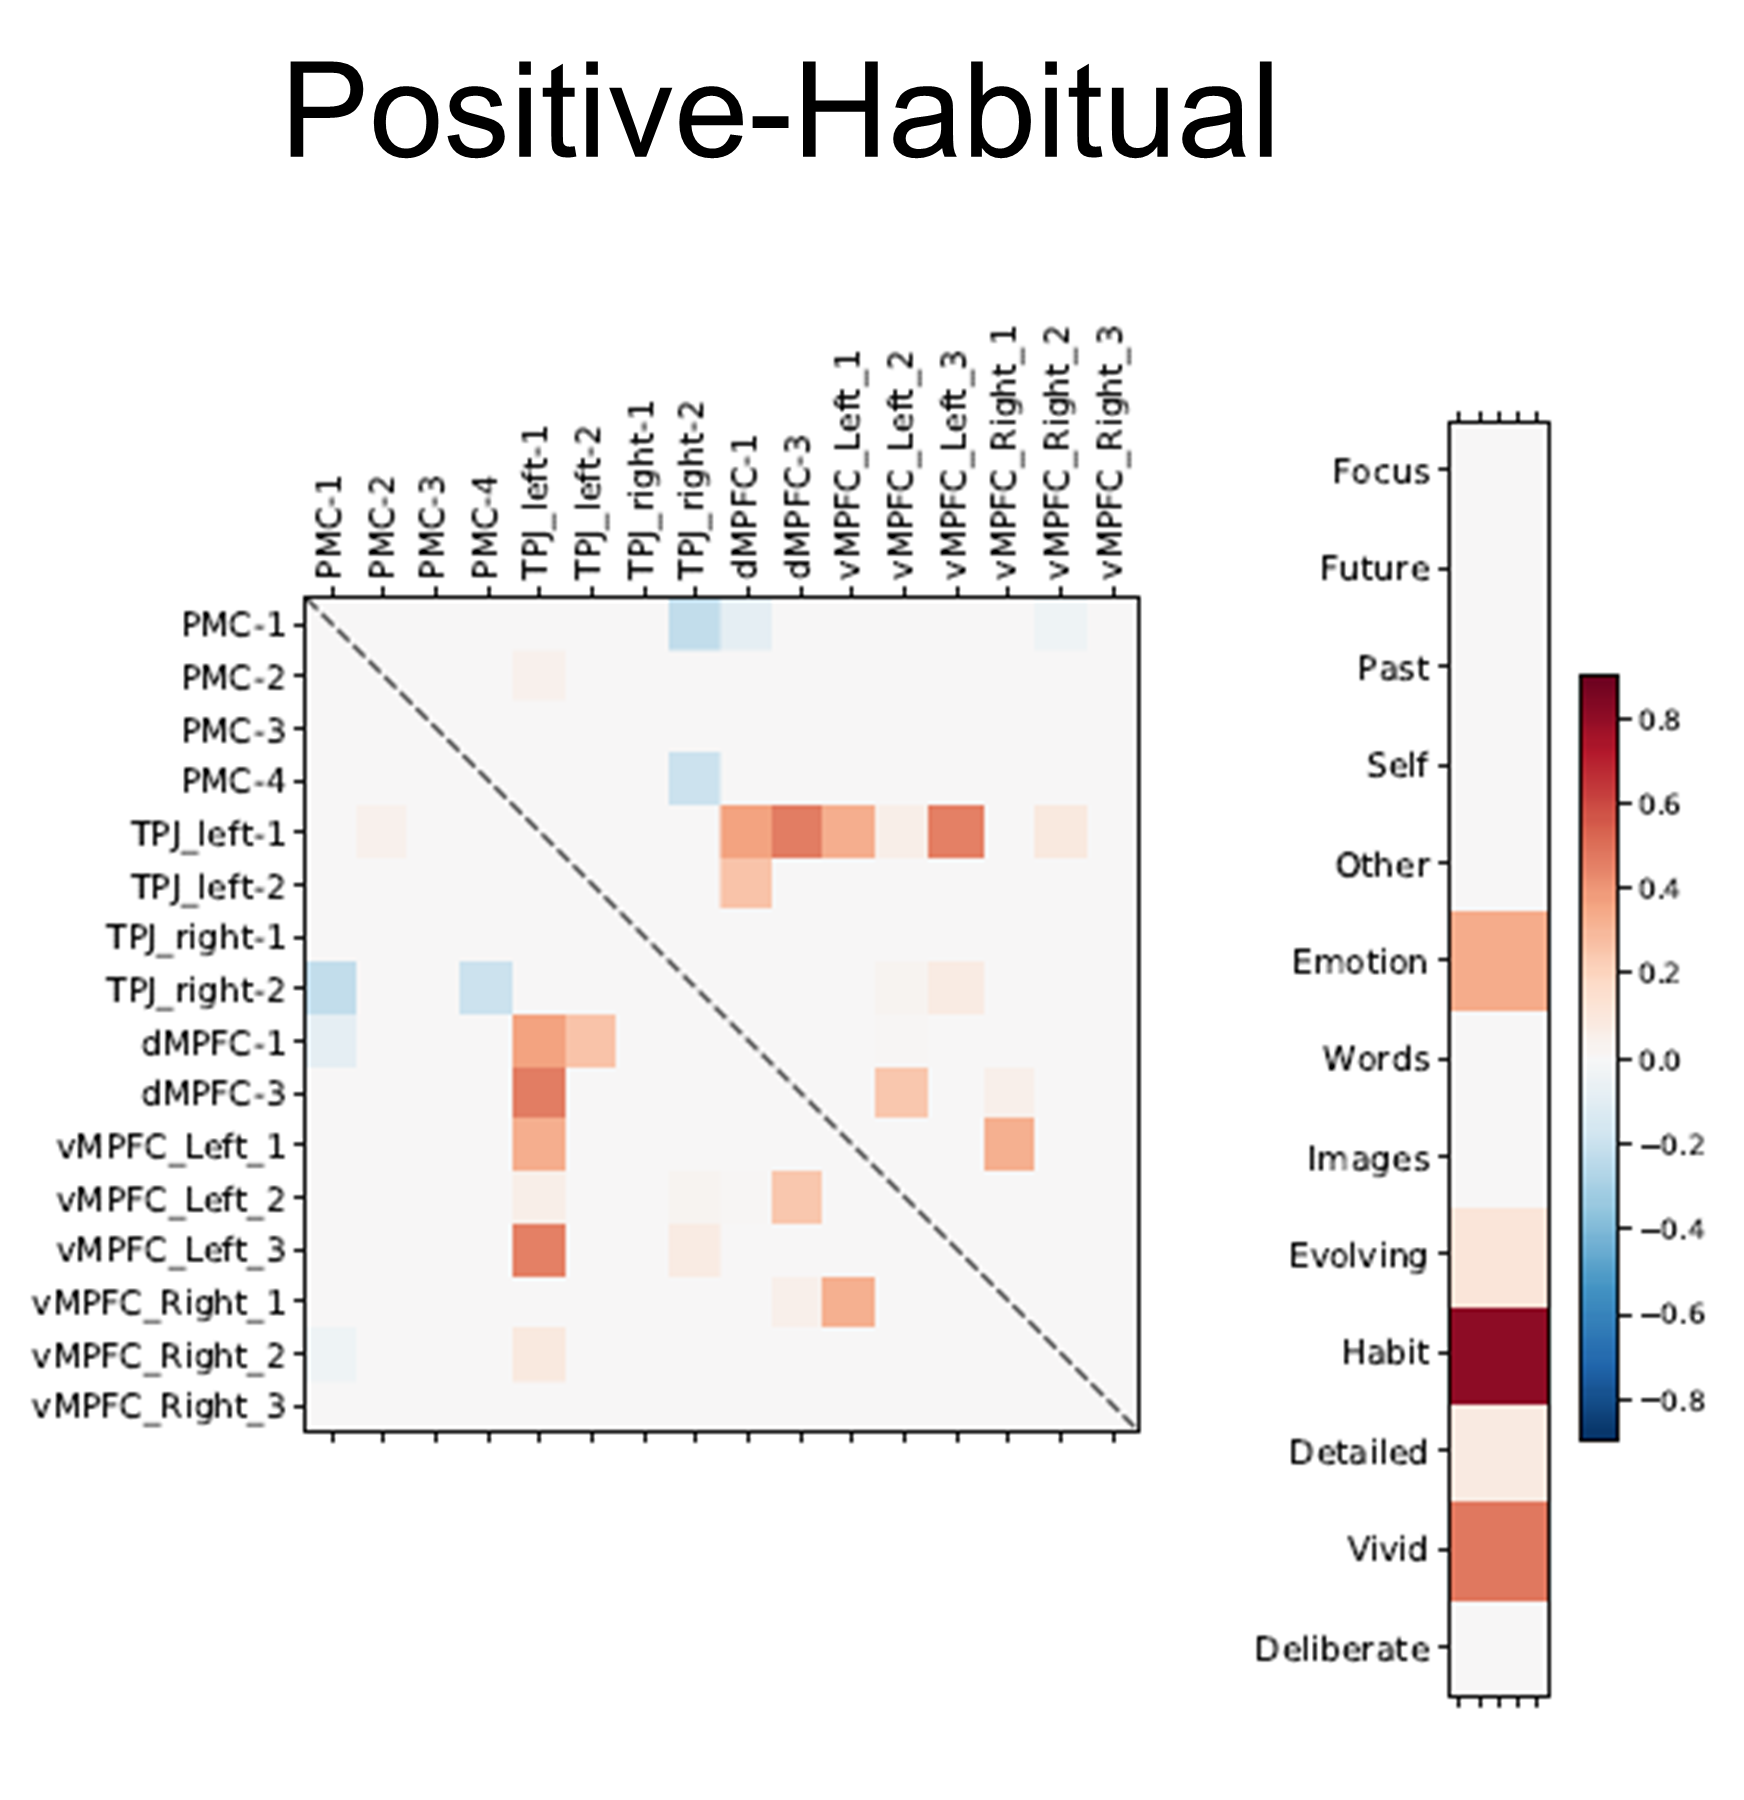
\includegraphics[width=0.6\textwidth]{append/image/study1figs4-1.png}
	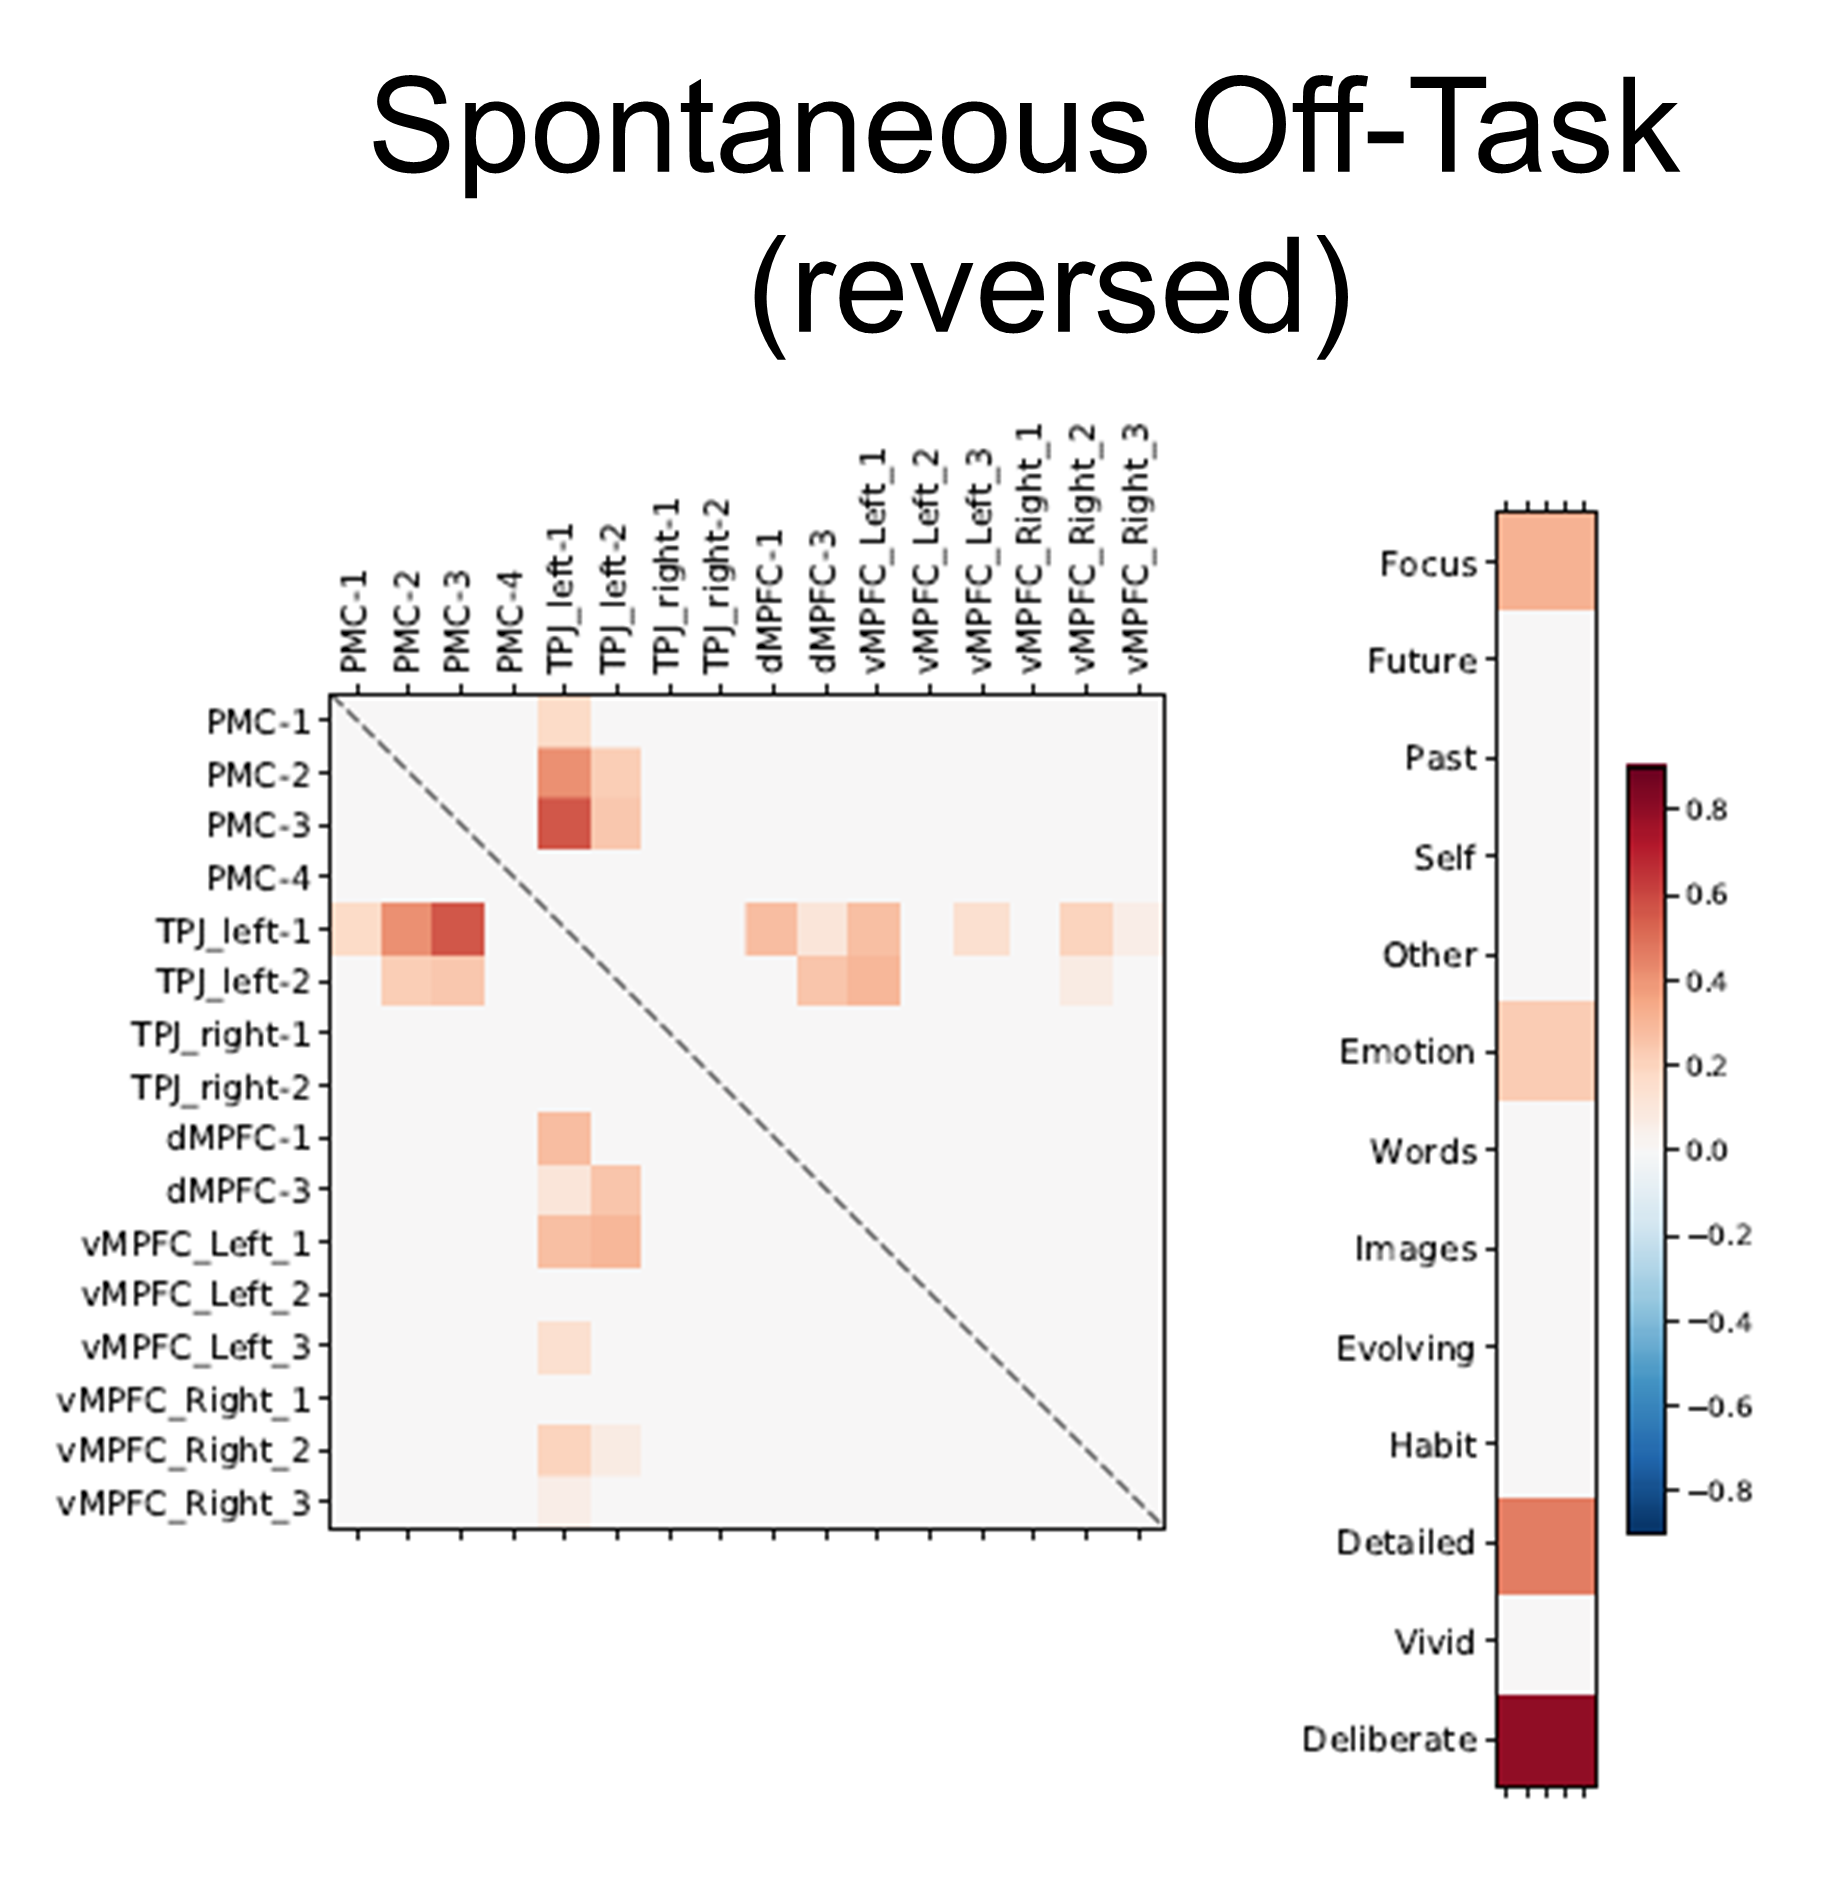
\includegraphics[width=0.6\textwidth]{append/image/study1figs4-2.png}
	\caption{Decomposition with motion outlier subjects excluded.}
	\label{fig:3S4}
\end{figure}
% ==========================================================================================================
\chapter{Nested K-Fold Cross-Validation}
\label{appendix:kfold}

\linespacesmall
\begin{algorithm}[htb]\footnotesize
\begin{algorithmic}[1]
\parbox{15.0cm}
{
\FOR{\textit{Each outer fold k}}
    \FOR{\textit{Each parameter set}}
        \STATE Separate the development set into j folds.
        \FOR{\textit{Each inner fold j}}
                \STATE Train the model on the training set
                \STATE Calculate test error in the validation set j
        \ENDFOR
        \STATE Compute the average inner cross-validation test error
    \ENDFOR

    \STATE Choose the best parameter set with minimum average test error.
    \STATE Use this parameter set to train on the development set.
    \STATE Calculate test error in the test set
\ENDFOR
\STATE Determine the optimal model based on the outer fold test error
\STATE Train the full dataset on the optimal model
}
\end{algorithmic}
\caption{: Nested k-fold cross-validation}
\label{algorithm:1}
\end{algorithm}
\linespacenormal

% ==========================================================================================================




% definitions and glossaries
% \cleardoublepage
% \makeabbreviations

% references
\cleardoublepage
\addcontentsline{toc}{chapter}{\numberline{}\bibname}

\linespacesmall
\bibliographystyle{apacite}
\bibliography{thesis.bib}
% the end
\end{document}